\chapter{Simulation du SDHCAL}
\label{chap.simulation}
La simulation est un aspect très important dans les expériences de physique des particules. En effet, la conception et l'optimisation d'un détecteur s'appuient toujours sur la simulation qui va permettre une estimation rapide des performances et des coûts de l'expérience. Les simulations sont aussi massivement utilisées dans l'analyse des données pour améliorer les algorithmes d'analyse, pour confirmer ou non la présence de nouvelle physique, pour estimer les biais etc. Pour les différentes expériences, avec des calorimètres ultra-granulaires, une simulation précise du phénomène de gerbe hadronique sera nécessaire. Pour développer et tester les algorithmes de suivi de particules, il faut que l'extension spatiale des cascades soient correctement simulée. La résolution en énergie doit aussi être bien simulée pour mener des procédures d'optimisation du détecteur. Cependant, la simulation des gerbes hadroniques est un phénomène compliqué à simuler. En effet, nous avons vu dans le chapitre~\ref{chap.shower}, qu'un grand nombre de processus physiques, accompagné de fluctuations, rentrent en jeu dans le développement d'une cascade hadronique. 

Dans ce chapitre, nous présenterons les modèles utilisés pour la simulation des gerbes hadroniques. Puis nous détaillerons la simulation du prototype SDHCAL et nous expliquerons les différentes étapes de la modélisation de la réponse des GRPC aux particules chargées. Enfin nous présenterons des comparaisons sur la réponse du SDHCAL aux gerbes hadroniques entre les données expérimentales et plusieurs modèles de simulation préparés par la collaboration GEANT4.
\minitoc
\newpage

%%%%%%%%%%%%%%%%%%%%%%%%%%%%%%%%%%%%%%%%%%%%%%%

\section{Les modèles de simulation des gerbes hadroniques}
La collaboration GEANT4~\cite{geant4} fournit un logiciel rassemblant de nombreux modèles théoriques et phénoménologiques qui décrivent les interactions des particules avec la matière. Ces modèles n'étant valables que sur certaines gammes d'énergie, ils doivent être combinés pour couvrir toute la gamme d'énergie du phénomène étudié. La  figure~\ref{fig.model} est un diagramme listant les différents modèles de simulation disponibles dans GEANT4 et leur gamme de validité en énergie. L'utilisateur doit combiner ces modèles pour simuler un phénomène physique. La collaboration GEANT4 fournit aussi un certain nombre de listes physiques définissant et utilisant des transitions entre ces modèles (cf. section~\ref{sec.listphys}).
\begin{figure}[!ht]
  \begin{center}
    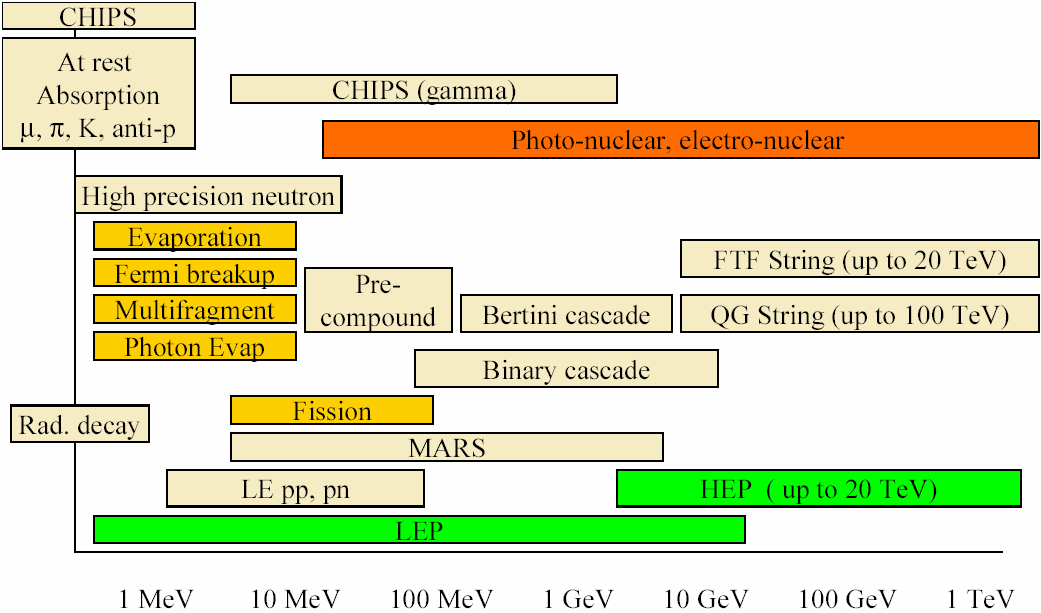
\includegraphics[width=.8\textwidth]{Digitizer/figs/HadronicModelsInventory.jpg}
    \caption{Les modèles utilisés dans GEANT4 en fonction de l'énergie des particules.}
    \label{fig.model}
  \end{center}
\end{figure}
\\
Les principaux modèles pour décrire les interactions hadroniques de haute énergie avec la matière sont les modèles de cordes partoniques (cf. section~\ref{sec.parton}). Ces modèles sont valables pour des énergies supérieures à $5-10$ GeV. Les interactions aux énergies intermédiaires (100 MeV < E < 10 GeV) sont décrites avec les modèles de cascades intranucléaires (cf. section~\ref{sec.inucl}). Pour traiter les noyaux excités par des collisions de plus haute énergie et les interactions en dessous de 200 MeV, une famille de modèles de désexcitation nucléaire (fission, évaporation nucléaire\dots) est disponible. Les interactions des neutrons de basse énergie (E<20 MeV) peuvent être simulées avec des modèles de haute précision pour neutrons où un grand nombre de sections efficaces ont été tabulées. L'utilisation ou non de ces modèles de haute précision pour les neutrons aura des conséquences sur le temps de calcul, sur la réponse simulée du détecteur ou sur la topologie des gerbes.
\subsection{Modèles de cordes partoniques}
\label{sec.parton}
Les modèles de cordes partoniques permettent de simuler les réactions de hautes énergies de hadrons avec des noyaux. Les deux principaux modèles utilisés dans GEANT4 sont les modèles QGS (Quark Gluon String) et FTF (Fritiof) \cite{geant4_parton}. Le résultat de l'interaction d'un hadron avec un noyau est une ou plusieurs cordes excitées. Une corde est un segment où chacune des deux extrémités est un quark ou un di-quark se déplaçant dans des directions opposées. Les noyaux sont modélisés comme un ensemble de nucléons dont les positions sont aléatoirement choisies en utilisant une distribution de densité. Pour les noyaux lourds~(A>16), une distribution de densité de la forme du potentiel de Wood-Saxon est utilisée : 
\begin{equation}
  \label{eq.wood-saxon}
  \rho(r_i)=\frac{\rho_0}{1+exp[(r_i-R)]/a}
\end{equation}
où $R$ et $a$ dépendent de la masse du noyau. Pour les noyaux légers une distribution de densité venant du modèle d'oscillateur harmonique est utilisée : 
\begin{equation}
  \label{eq.harmonic-ocsillator}
  \rho(r_i)=(\pi R'^2)^{-3/2}exp(-r_i^2/R'^2)
\end{equation}
avec $R'$  qui dépend de la masse du noyau.
Pour calculer le paramètre d'impact avec les nucléons, ces deux distributions de densité sont réduites dans un plan perpendiculaire à la direction de la particule incidente. La probabilité de collision entre le hadron et un nucléon est calculée en utilisant une distribution gaussienne pour les fonctions d'onde du hadron et des nucléons. Ces probabilités sont utilisées pour connaître le nombre de nucléons participant à la réaction dans le noyau.\\
Des cordes sont ensuite créées, les quarks du hadron incident sont aléatoirement répartis entre celles-ci. Un modèle de fragmentation longitudinale de cordes est ensuite utilisé pour créer des hadrons et des nouvelles cordes. Une corde se fragmente en une paire quark anti-quark $q-\bar q$ ou diquark anti-diquark $qq-\bar q \bar q$ \cite{geant4_reference}. Les probabilités relatives de création des quark ou diquark sont :
\begin{equation}
  u:d:s:qq = 1:1:0.35:0.1
\end{equation}
La paire de quark anti-quark (ou diquark anti-diquark) créée, est placée à l'intérieur de la précédente paire. Une moitié de ces nouvelles paires sont utilisées pour créer un hadron tandis que les autres constituants créent une nouvelle corde. Ce processus se répète jusqu'à ce que l'énergie d'une corde ne soit pas suffisante pour créer un hadron. Le tableau~\ref{tab.partonModelTable} présente les domaines, en énergie des hadrons, de validité des modèles QGS et FTF pour différentes particules incidentes.
\begin{table}[!ht]
  \begin{center}
    \begin{tabular}{c|c|c}
      \rowcolor{black!20!white}Particule & QGS & FTF\\
      \rowcolor{black!5!white}\hline
      \rowcolor{black!5!white}$K+$ & $12\ GeV\ -\ 100\ TeV$ & $4\ GeV\ -\ 100\ TeV$\\
      \rowcolor{black!5!white}$K-$ & $12\ GeV\ -\ 100\ TeV$ & $4\ GeV\ -\ 100\ TeV$\\
%      \rowcolor{black!5!white}$\lambda$ & $ $ & $2\ GeV\ -\ 100\ TeV$\\
      \rowcolor{black!5!white}$\pi+$ & $12\ GeV\ -\ 100\ TeV$ & $4\ GeV\ -\ 100\ TeV$\\
      \rowcolor{black!5!white}$\pi-$ & $12\ GeV\ -\ 100\ TeV$ & $4\ GeV\ -\ 100\ TeV$\\
      \rowcolor{black!5!white}$neutron$ & $12\ GeV\ -\ 100\ TeV$ & $4\ GeV\ -\ 100\ TeV$\\
      \rowcolor{black!5!white}$proton$ & $12\ GeV\ -\ 100\ TeV$ & $4\ GeV\ -\ 100\ TeV$\\
      \rowcolor{black!5!white}$ion$ & $ $ & $2\ GeV\ -\ 100\ TeV$\\
    \end{tabular}
  \end{center}
  \caption{Domaine de validité des modèles QGS et FTF pour plusieurs hadrons incidents.}
  \label{tab.partonModelTable}
\end{table}

Après l'interaction du noyau avec la particule incidente, celui-ci sera dans un état excité. Le retour à l'état fondamental du noyau est simulé avec des modèles de fragmentation et de désexcitation nucléaire.
\subsection{Les modèles de cascade intranucléaire}
\label{sec.inucl}
Il a été montré dans \cite{bertini} en 1969 qu'un modèle de cascade intranucléaire décrivait relativement bien les interactions de nucléons de 100 MeV à 2 GeV avec des noyaux. Ces réactions sont caractérisées par une rapide ($10^{-23}-10^{-22} s$) cascade intranucléaire laissant les noyaux dans un état excité, suivi d'une phase plus lente ($10^{-18}-10^{-16} s$) d'évaporation nucléaire. Les modèles de cascade binaire et celui de Bertini sont les modèles disponibles dans GEANT4 pour simuler les cascades intranucléaires.
\subsubsection{Le modèle de Bertini}
\begin{figure}[!ht]
  \begin{center}
    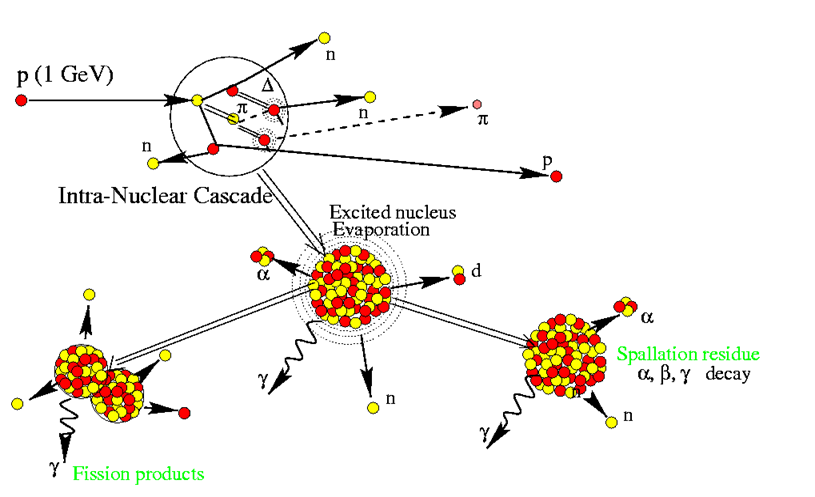
\includegraphics[width=.8\textwidth]{Digitizer/figs/intraNucl.png}
    \caption{Schéma d'explication du modèle de Bertini. Un hadron de 1 $GeV$ crée une cascade intranucléaire.}
    \label{fig.g4bertini}
  \end{center}
\end{figure}
Le modèle de Bertini a été étendu, il est valable pour des particules incidentes ($p$, $n$, $\pi$, $K$, $\Delta$, $\Sigma$, $\Xi$, $\Omega$ et $\gamma$) avec une énergie cinétique comprise entre 100 MeV et 10 GeV~\cite{geant4_bertini}. Ce modèle est applicable lorsque la longueur d'onde de de Broglie de la particule incidente est du même ordre que la distance moyenne entre les nucléons du noyau et lorsque l'énergie de la particule incidente est supérieure à l'énergie de Fermi. 

Le noyau cible est modélisé par une ou trois couches concentriques de densité constante en fonction du nombre de nucléons dans le noyau (1 couche si A<4, 3 sinon). La cascade commence lorsqu'une particule incidente rencontre un nucléon du noyau cible. Le point d'impact de la particule incidente est choisi aléatoirement dans une distribution sphérique uniforme. Les sections efficaces entre la particule et les nucléons, la densité de nucléons et les impulsions des nucléons sont utilisées pour calculer le libre parcours de la particule. Les impulsions des nucléons sont calculées en utilisant le modèle du gaz de Fermi. Une collision entre la particule incidente et un nucléon peut produire des particules secondaires. Pour les pions, le modèle de Bertini prend en charge les collisions élastiques et les collisions inélastiques suivantes: $\pi^-p\rightarrow\pi^0n$, $\pi^0p\rightarrow\pi^+n$, $\pi^0n\rightarrow\pi^-p$, et $\pi^+n\rightarrow\pi^0p$. Des réactions produisant plus de 2 particules sont aussi implémentées. Les pions peuvent aussi être absorbés par les nucléons par le biais des réactions de la forme: $\pi^-pp\rightarrow np$. Les impulsions du nucléon et des particules secondaires créées sont calculées. Ces particules secondaires sont alors susceptibles d'interagir à leur tour avec les nucléons du noyau si leur énergie cinétique est supérieure à 2 $MeV$. La valeur de cette coupure vient du principe d'exclusion de Pauli. Les produits d'une réaction initiée par une particule d'énergie inférieure à une valeur approximative de 2 $MeV$ auraient une énergie encore plus faible. Or dans un gaz de Fermi, les niveaux d'énergie les plus bas sont remplis, empêchant d’accueillir de nouveaux nucléons avec une énergie inférieure à celle de Fermi. L'énergie minimale pour la production de nouvelles particules correspond au plus faible niveau d'énergie non rempli. Pour simplifier le modèle et tenir compte du principe de Pauli, l'énergie de Fermi est choisie à 2 $MeV$. La cascade intranucléaire prend fin lorsque toutes les particules secondaires sont absorbées ou se sont échappées du noyau. Le noyau est alors dans un état excité: des nucléons du noyau ont changé de niveau d'énergie. Un modèle de désexcitation est alors utilisé pour traiter les transitions de ces nucléons. Les noyaux résultants peuvent être instables et seront traités avec des modèles de fission et d'évaporation nucléaire.

\subsubsection{Le modèle de cascade binaire}
Dans GEANT4, un autre modèle de cascade intranucléaire est disponible, il est utilisé par certaines listes physiques. C'est le modèle de cascade binaire. Dans ce modèle, les nucléons du noyau cible sont au repos. La densité des noyaux est de la forme du potentiel de Wood-Saxon (cf. équation~\ref{eq.wood-saxon}) pour les noyaux lourds (A>16). Pour les noyaux légers la densité donnée par le modèle d'oscillateur harmonique est utilisée (cf. équation~\ref{eq.harmonic-ocsillator}). Les trajectoires des particules primaires et secondaires sont des lignes droites. A chaque étape de la cascade, la plus proche distance $d_i^{min}$ entre le nucléon $i$ et la trajectoire des particules est calculée pour tous les nucléons du noyau. Des collisions entre les particules et les noyaux sont possibles si cette distance satisfait la condition suivante: $d_i^{min}<\sqrt{\frac{\sigma_i}{\pi}}$, où $\sigma_i$ est la section efficace d'interaction entre le nucléon cible et la particule. De même que pour le modèle de Bertini, le principe d'exclusion de Pauli est vérifié et, si une interaction crée une particule avec une énergie inférieure à un seuil, cette réaction est supprimée. La cascade prend fin lorsque toutes les particules secondaires s'échappent du noyau ou l'énergie des particules secondaires est insuffisante pour continuer la cascade.

\subsubsection{Les modèles paramétrés}
Dans GEANT4, deux modèles étaient utilisés pour simuler l'ensemble des processus de manière paramétrée. Ce sont les modèles Low Energy Parametrized (LEP) et High Energy Parametrized (HEP). Ces modèles ont montré des limites. Les résolutions en énergie des gerbes hadroniques simulées avec ces modèles étaient souvent meilleures que dans les données expérimentales. Les simulations produisaient également des gerbes hadroniques plus étroites que les données. Le modèle LEP est encore utilisé dans quelques listes physiques (cf. section\ref{sec.listPhys}) mais est progressivement remplacé.
\subsection{Les listes physiques}
\label{sec.listPhys}
Les différents modèles implémentés dans GEANT4 ne sont valables que sur certaines gammes d'énergie. La simulation d'un phénomène tel que les gerbes hadroniques a besoin de modèles valides sur une très grande gamme d'énergie. La particule primaire peut pénétrer le calorimètre avec une énergie allant de quelques $GeV$ jusqu'à plusieurs centaines de $GeV$. Il faut alors combiner ces modèles et définir les lois de transition entre les modèles pour couvrir toute la gamme d'énergie. Ces combinaisons de modèles et leur loi de transition sont appelées listes physiques. Les utilisateurs peuvent alors créer leur propre liste physique ou bien en utiliser une parmi celles préparées par la collaboration GEANT4. La figure~\ref{fig.g4list} présente les deux listes physiques les plus utilisées dans le domaine de la calorimétrie à haute énergie. 
\label{sec.listphys}
\begin{figure}[!ht]
  \begin{center}
    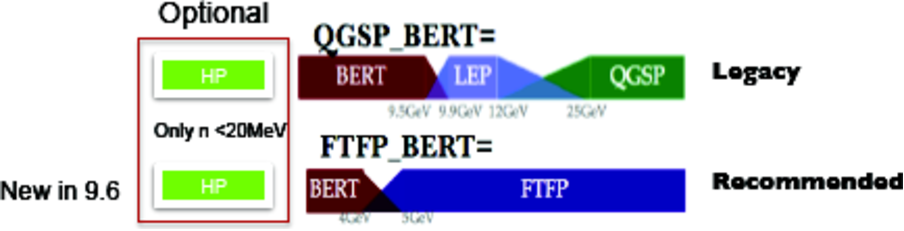
\includegraphics[width=.8\textwidth]{Digitizer/figs/physics_list_G4.pdf}
    \caption{Schéma descriptif des listes physiques FTFP\_BERT(\_HP) et QGSP\_BERT(\_HP).}
    \label{fig.g4list}
  \end{center}
\end{figure}
Les transitions entre les modèles sont linéaires. Pour la liste FTFP\_BERT, GEANT4 va aléatoirement choisir entre les modèles de Bertini et Fritiof pour simuler l’interaction d'une particule d'énergie entre 4 et 5 $GeV$. Par exemple, le modèle Bertini aura une probabilité de 25$\%$ d'être choisi alors que la probabilité de choisir le modèle de Fritiof sera de 75$\%$. Il est à noter que la gamme de validité d'un modèle peut varier dans une liste selon la nature de la particule. Enfin, pour quelques listes physiques, l'option $HP$ (High Precision for neutrons) est disponible. L'utilisation de cette option permet d'être plus précis sur les interactions des neutrons avec la matière lorsque ceux-ci ont une énergie inférieure à 20 $MeV$. Cette option augmente le temps de calcul de la simulation du SDHCAL, d'un facteur légèrement inférieur à 10. Le tableau suivant présente plusieurs listes physiques avec les domaines de validité des différents modèles pour les protons.
\begin{table}[!ht]
  \begin{center}
    \begin{tabular}{c|c|c}
      \rowcolor{black!20!white}Liste physique & Modèle & Gamme d'énergie \\
      \rowcolor{black!5!white}\hline
      \rowcolor{black!5!white}FTFP\_BERT(\_HP) & Bertini & 0$\rightarrow$5 $GeV$\\
      \rowcolor{black!5!white}$ $        & Fritiof & 4$\rightarrow$100 $TeV$\\
      \rowcolor{black!5!white}\hline
      \rowcolor{black!5!white}QGSP\_BERT(\_HP) & Bertini & 0$\rightarrow$9.9 $GeV$\\
      \rowcolor{black!5!white}$ $        & LEP & 9.5$\rightarrow$25 $GeV$\\
      \rowcolor{black!5!white}$ $        & QGS & 12$\rightarrow$100 $TeV$\\
      \rowcolor{black!5!white}\hline
      \rowcolor{black!5!white}QGSP\_FTFP\_BERT & Bertini & 0$\rightarrow$8 $GeV$\\
      \rowcolor{black!5!white}$ $              & Fritiof & 6$\rightarrow$25 $GeV$\\
      \rowcolor{black!5!white}$ $              & QGS & 12$\rightarrow$100 $TeV$\\
      \rowcolor{black!5!white}\hline
      \rowcolor{black!5!white}QGSP\_BIC(\_HP) & Cascade Binaire & 0$\rightarrow$9.9 $GeV$\\
      \rowcolor{black!5!white}$ $             & LEP & 9.5$\rightarrow$25 $GeV$\\
      \rowcolor{black!5!white}$ $             & QGS & 12$\rightarrow$100 $TeV$\\
      \rowcolor{black!5!white}\hline
      \rowcolor{black!5!white}FTF\_BIC  & Cascade Binaire & 0$\rightarrow$ 5 $GeV$\\
      \rowcolor{black!5!white}$ $       & FTF & 4$\rightarrow$100 $TeV$\\
    \end{tabular}
  \end{center}
  \caption{Exemple de listes physiques disponibles dans GEANT4 version 9.6. L'option $HP$ est indiquée lorsqu'elle est disponible. Cette option n'est utilisée que pour les neutrons d'énergie inférieure à 20 $MeV$.}
  \label{tab.physList}
\end{table}

%%%%%%%%%%%%%%%%%%%%%%%%%%%%%%%%%%%%%%%%%%%%%%%

\section{La simulation du prototype}
La simulation du prototype a été réalisée avec un programme basé sur GEANT4 (version~9.6). La géométrie du détecteur est décrite dans ce programme avec une grande précision. Les compositions chimiques et les densités des matériaux du prototype sont détaillées. Ces informations seront utilisées par GEANT4 pour des calculs de sections efficaces lors de la propagation des particules dans le détecteur. Le champ électrique entre les deux électrodes de verre des GRPC n'est pas simulé. Les avalanches issues des ionisations du gaz par les particules incidentes sont modélisées dans un algorithme dédié qui sera décrit dans la section~\ref{sec.digit-algo} de ce chapitre. Cet algorithme est aussi responsable de la répartition de la charge sur les carreaux de cuivre et donc de la multiplicité (cf. section~\ref{sec.muons} du chapitre~\ref{chap.sdhcal}). 

Nous avons décrit dans la section précédente les différents modèles utilisés dans GEANT4 pour propager les particules dans la matière. La trajectoire de ces particules (primaires et/ou secondaires) est segmentée dans GEANT4. A chaque interaction avec les matériaux du détecteur, un nouveau segment est créé. La création d'un nouveau segment se fait aussi à chaque fois qu'une particule change de volume (e.g. passant du verre au gaz). Il arrive que plusieurs segments soient créés pour une seule particule dans le volume de gaz d'une seule GRPC. Ces segments pourraient déclencher la simulation de plusieurs avalanches dans une couche de gaz et ainsi modifier la réponse simulée du détecteur. Pour éviter ce phénomène, les segments appartenant à la même particule dans une même couche de gaz sont reliés entre eux.
La liste des segments après la procédure d'association, se trouvant dans le milieu actif du détecteur (le gaz entre les électrodes pour le SDHCAL), est alors enregistrée. Seuls les segments associés à des particules chargées sont conservés. Les informations stockées pour ces segments sont les suivantes: les coordonnées des positions du début et de la fin du segment; l'énergie déposée dans le gaz par la particule le long du segment; la nature de la particule; le temps d’occurrence du segment relatif au moment où la particule primaire a été générée. 
Cette liste de segment est ensuite utilisée comme point de départ de l’algorithme qui modélise la réponse des GRPC aux particules chargées.

%%%%%%%%%%%%%%%%%%%%%%%%%%%%%%%%%%%%%%%%%%%%%%%

\section{Modélisation de la réponse des GRPC aux particules chargées}
Nous venons de voir que le résultat du programme de simulation du SDHCAL est une liste de segments correspondant à une partie de la trajectoire d'une particule dans le détecteur. Nous avons vu que l'énergie déposée par ces segments étaient disponible alors que dans le cas du SDHCAL, seule la charge induite sur les carreaux de cuivre est mesurée. De plus, le phénomène de multiplicité introduit au chapitre~\ref{chap.sdhcal} n'est pas pris en compte par GEANT4. 
\label{sec.digit-algo}
%%%%%%%%%%%%%%%%%%%%%%%%%%%%%%%%%%%%%

\subsection{Algorithme SimDigital}
\label{sec.algo}
La modélisation est faite à l'aide d'un algorithme appelé SimDigital qui est un processeur Marlin \cite{marlin} disponible dans le paquet MarlinReco \cite{marlinreco} de l'ILCSoft \cite{ilcsoft}. Le but de cet algorithme est de simuler la réponse des GRPC lors du passage de particules chargées dans l'intervalle de gaz. Les différentes étapes de l’algorithme sont les suivantes:
\begin{enumerate}[~~1-]
\item La fenêtre en temps utilisée dans la procédure de reconstruction des événements décrite dans la section~\ref{sec.trivent} du chapitre~\ref{chap.sdhcal}, est de 1000 $ns$ (5 coups d'horloge de 200 $ns$ pour reconstruire un événement physique). Ainsi, les particules interagissant tardivement dans le détecteur comme les neutrons peuvent ne pas être associées à l’événement. Pour prendre cet effet en compte, les segments dont le temps d’occurrence est supérieur à 1000 $ns$ sont supprimés.
\item \label{it.start} Une cellule de lecture $C_0$, associée à un volume de gaz où un ou plusieurs segments ont traversé le gaz, est sélectionnée. La longueur de ses segments est alors calculée.
\item La longueur de certains segments dans le gaz peut être très petite. Ce phénomène peut avoir lieu aléatoirement lors de la propagation des particules par GEANT4. Cependant la majorité des cas où ce phénomène s'observe, s'explique par le changement de volume d'une particule. La figure~\ref{fig.map_and_length_vs_deltaz}(a) présente la longueur des segments en fonction de la distance entre la position du milieu du segment et le milieu de la couche de gaz ($\Delta_z$). Cette figure montre qu'une grande fraction des segments de faible longueur sont proches des deux électrodes en verre ($|\Delta_z|\simeq0.6~mm$). Ces segments de longueur presque nulle n'ont pas de raison de déclencher une avalanche dans le gaz. Les segments de longueur inférieure à une longueur donnée $l_{min}$ ($l_{min}=1 \mu m$ par défaut)sont donc supprimés.
  \begin{figure}[!ht]
    \subfigure[]{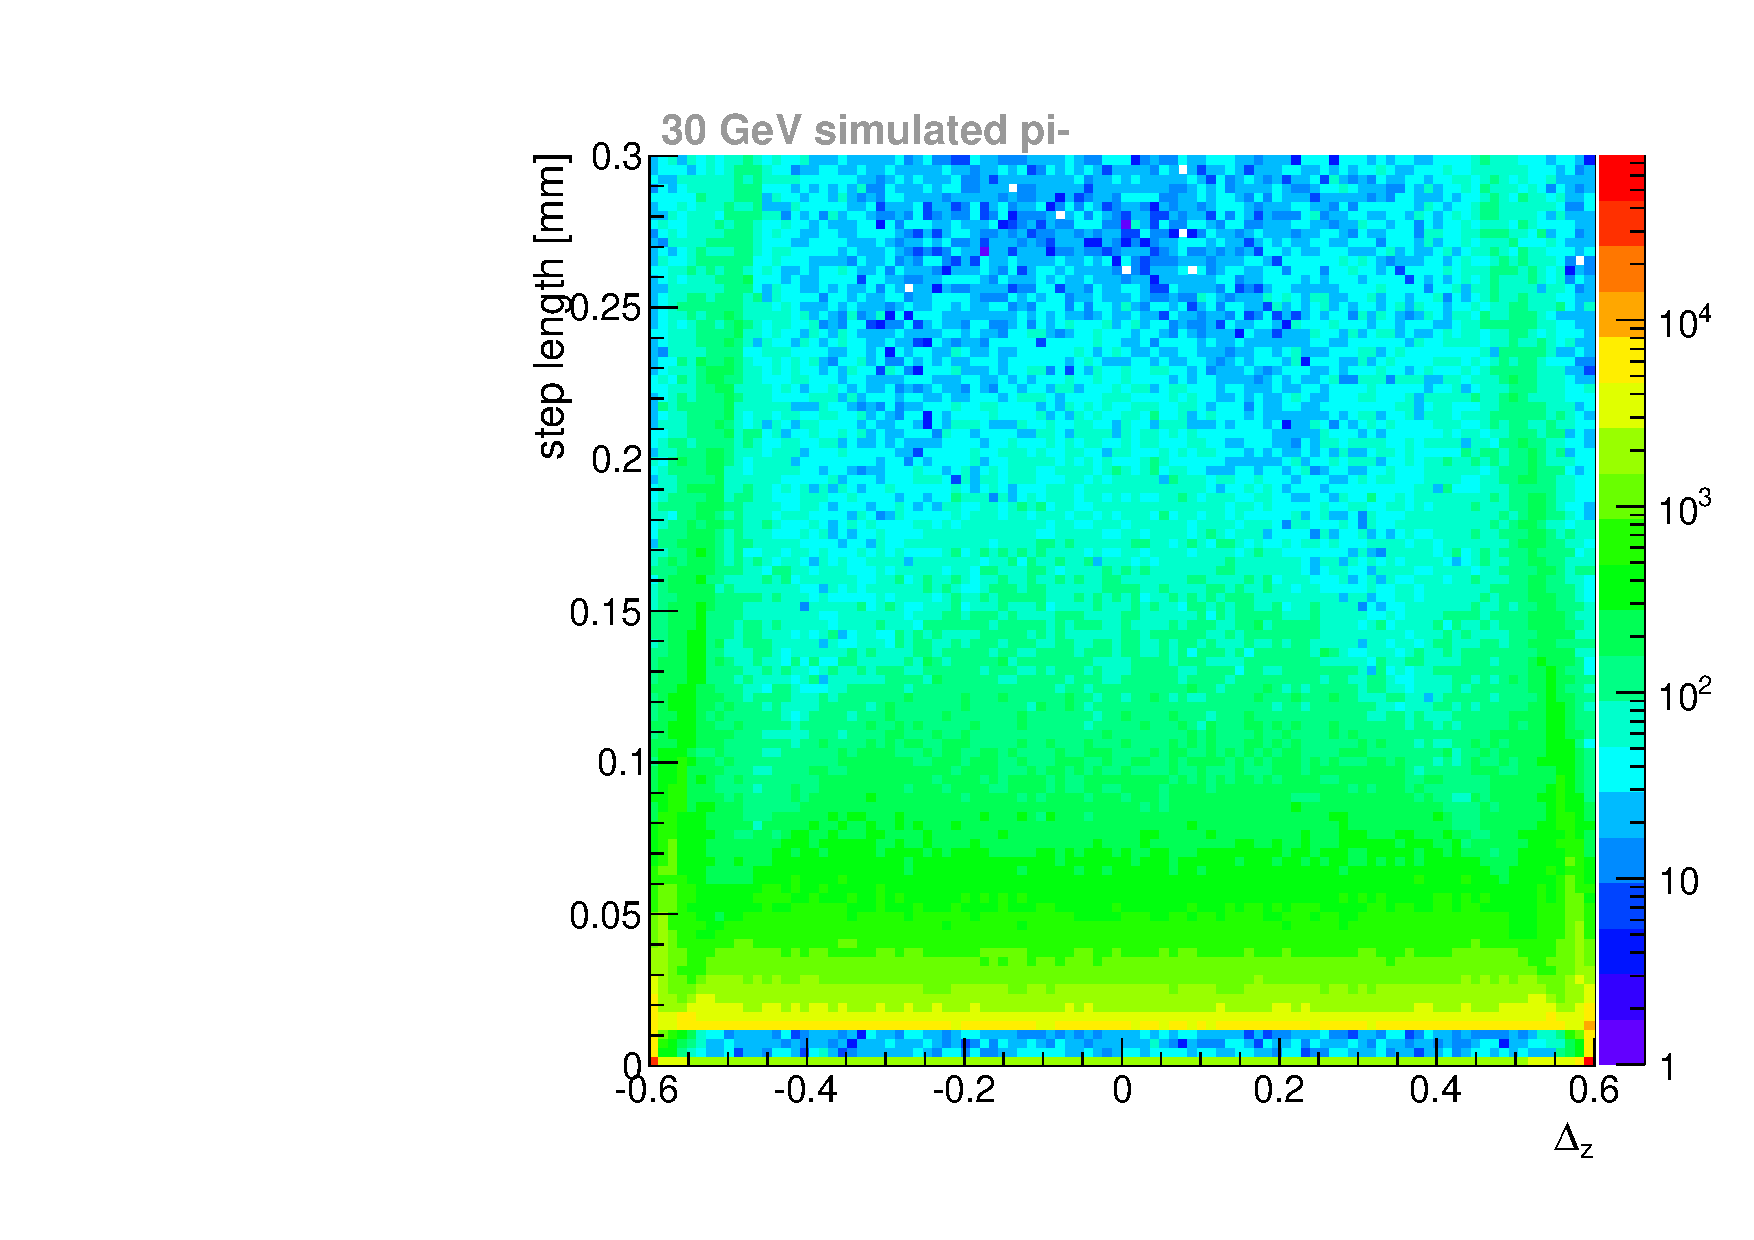
\includegraphics[width=0.5\textwidth]{Digitizer/figs/stepLength_zoom.pdf}}
    \subfigure[]{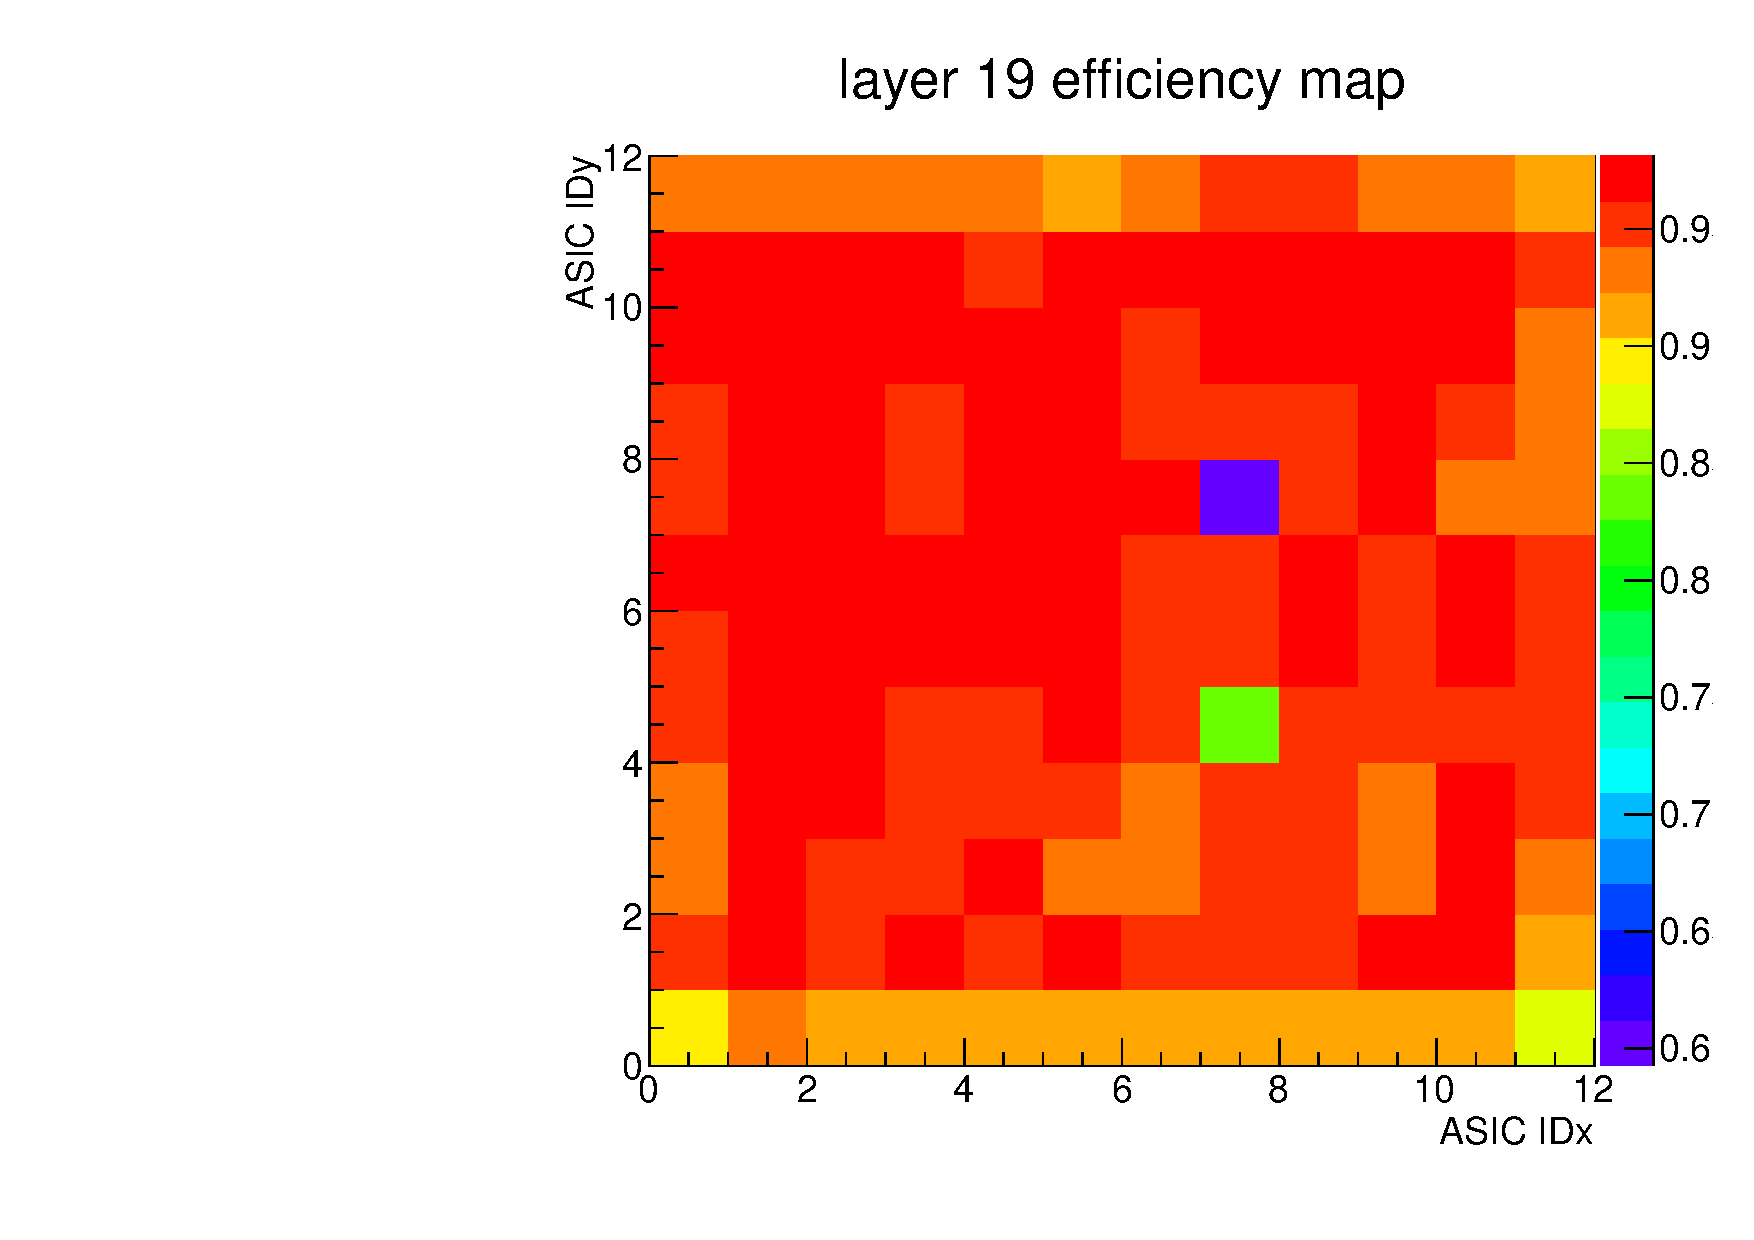
\includegraphics[width=0.5\textwidth]{Digitizer/figs/layer19map.pdf}}
    \caption{(a): Longueur des segments (step length) en $mm$ en fonction de $\Delta_z$ en $mm$. Cette figure est centrée sur la région des segments de faible longueur pour mettre en évidence le fait que la plupart des segments de longueur nulle (ou presque) sont localisés sur les bords de la couche de gaz ($|\Delta_z|\simeq0.6\ mm$). (b): Exemple d'une carte d'efficacité des ASICs.}
    \label{fig.map_and_length_vs_deltaz}
  \end{figure}
\item Les cartes d'efficacité des ASICs du prototype déterminées en utilisant la même méthode que celle décrite dans la partie~\ref{sec.muons} du chapitre~\ref{chap.sdhcal}, sont utilisées pour prendre en compte les effets des absorbeurs ($CO_2$,$SF_6$). En effet, les propriétés de ces deux gaz (capture des photons et d'électrons) ne sont pas incluses dans GEANT4. De plus, l'utilisation de ces cartes d’efficacité permet d'éviter la présence de signal dans les canaux électroniques hors d'usage ou masqués. Ainsi, lorsqu'un segment est dans une région du détecteur où l'efficacité est de 50\%, alors ce segment a 50\% de chance d'être conservé. La figure~\ref{fig.map_and_length_vs_deltaz}(b) montre un exemple de carte d'efficacité d'une chambre du prototype SDHCAL.
\item La charge induite pour chaque segment est alors aléatoirement choisie dans une distribution de Polya: 
  \begin{equation}
    \label{eq.polya}
    P(q)=[\frac{q}{\bar q}(1+\theta)]^{\theta}e^{[-\frac{q}{\bar q}(1+\theta)]}
  \end{equation}
  où $\bar q$ est la valeur moyenne en $pC$ et $\theta$ un paramètre libre lié à la largeur de la distribution. Cette charge induite est ensuite corrigée: 
  \begin{equation}
    \label{eq.lengthcorrection}
    Q_{corr} = \left\{ \begin{array}{rl}
      Q_{ind}(\frac{d_s}{d_{gap}})^\kappa &\mbox{ si $\frac{d_s}{d_{gap}}>1$} \\
      Q_{ind} &\mbox{ sinon}
    \end{array} \right.
  \end{equation}
  où $d_s$ correspond à la longueur du segment, $d_{gap}$ à l'épaisseur du volume de gaz (1.2 $mm$) et $\kappa$ est un paramètre libre. Lorsque le segment traverse toute la couche de gaz, la grandeur $\frac{d_{gap}}{d_s}$ correspond au cosinus de l'angle entre la trajectoire du segment et la droite normale aux GRPC. La forme $\frac{d_s}{d_{gap}}$ est préférée à $\frac{1}{cos\theta}$ pour éviter un facteur correctif infini. L'effet et l'importance de cette correction seront discutés dans la partie~\ref{sec.param} de ce chapitre.
\item Dans les gerbes hadroniques et électromagnétiques, les particules chargées peuvent être très proches. Ainsi les avalanches générées dans le gaz par ces particules peuvent se chevaucher. Cependant, dans le régime avalanche, le signal induit par ces particules n'est pas équivalent à la somme des signaux induits par ces particules prises individuellement. Pour tenir compte de cet effet écran, lorsque la distance entre deux segments est inférieure à une valeur $d_{cut}$, le segment dont la charge induite ($Q_{corr}$) est la plus faible, est supprimé. %Ce filtre permet aussi de supprimer un ou plusieurs segments provenant d'une seule particule. En effet, une interaction entre une particule chargée et le gaz peut avoir lieu dans GEANT4. Ainsi plusieurs segments seraient créés et pourraient déclencher plusieurs avalanches alors qu'une seule particule est passée.
\item \label{it.spliting} La charge induite est ensuite répartie sur la cellule $C_0$  et sur les cellules voisines se trouvant dans le même plan et à une distance inférieure à une valeur $r_{max}$ de $C_0$. Le rapport suivant est alors calculé pour chaque canal:
  \begin{equation}
    \label{eq.ratio}
    R_i = \frac{\int_{a_i}^{b_i}\int_{c_i}^{d_i}\sum_{j=0}^{n-1}\alpha_j e^{ \frac{(x-x_0)^2+(y-y_0)^2}{2\sigma_j^2}}dxdy}{N}
  \end{equation}
  où $a_i,\ b_i,\ c_i,\ d_i$ sont les positions des bords de la cellule $i$, $(x_0,y_0)$ sont les coordonnées du milieu du segment et N un facteur de normalisation définit comme: 
  \begin{equation}
    \label{eq.norm}
    N=\int_{-r_{max}}^{+r_{max}}\int_{-r_{max}}^{+r_{max}}\sum_{j=0}^{n-1}\alpha_j e^{ \frac{(x_0-x)^2+(y_0-y)^2}{\sigma_j^2}}dxdy
  \end{equation}
  Pour chaque canal ($C_0$ et ses voisins), la charge induite est augmentée d'une valeur $R_iQ_{corr}$.
\item L'opération est répétée à partir de l'étape~\ref{it.start} pour tous les canaux avec des segments.
\item Les seuils sont finalement appliqués pour toutes les cellules. Les cellules pour lesquelles la charge induite est supérieure à la valeur du premier seuil sont étiquetées selon la valeur de cette charge. Les autres cellules ne créent pas de hits. 
\end{enumerate}

%%%%%%%%%%%%%%%%%%%%%%%%%%%%%%%%%%%%%

\subsection{Paramétrage de l'algorithme}
\label{sec.param}
Nous avons vu les différentes étapes de l'algorithme responsable de la simulation de la réponse des GRPC au passage de particules chargées. Cet algorithme introduit de nombreux paramètres. Les méthodes utilisées pour obtenir le meilleur paramétrage possible sont décrites dans la section suivante. 
%%%%%%%%%%%%%%%%%%%%%%%%%%%%%%%%%%%%%

\subsubsection{Mesure du spectre de charge}
% 
\label{sec.polya}
Le régime utilisé pour les GRPC du prototype est le régime avalanche saturée. Ce régime a été décrit dans \cite{abbresciaPolya} et il a été montré qu'une distribution de Polya (cf. équation.~\ref{eq.polya}) s'ajuste bien aux spectres de charge expérimentaux. Il n'était pas possible de faire une mesure directe du spectre de charge avec une chambre du prototype. Cette mesure qui nécessite une lecture analogique d'une GRPC avait été réalisée avec une chambre différente de celles du prototype. La chambre utilisée était plus petite, le signal était enregistré avec un seul canal de lecture de $8 \times 8 ~cm^{2}$. Le mélange de gaz et la haute tension appliquée étaient différents. Le spectre de charge obtenu était compatible avec une distribution de Polya \cite{kieffer}. Nous avons donc fait l'hypothèse que le spectre de charge  des chambres du prototype suit une distribution de Polya et nous avons utilisé un scan en seuil pour déterminer ses paramètres. Cette méthode consiste à étudier l'efficacité de détection des muons en fonction de la valeur des seuils. Nous avons choisi 9 chambres dans lesquelles nous avons fait varier la valeur du seuil 1, 2 ou 3.
\begin{table}[!ht]
  \begin{center}
    \begin{tabular}{c|c}
      \rowcolor{black!20!white}Seuil & Numéro de chambre\\
      \rowcolor{black!5!white}\hline
      \rowcolor{black!5!white}$1$ & $6,~16,~30$\\
      \rowcolor{black!5!white}$2$ & $10,~22,~34$\\
      \rowcolor{black!5!white}$3$ & $14,~26,~38$\\
    \end{tabular}
  \end{center}
  \caption{Liste des chambres utilisées pour le scan en seuil.}
  \label{tab.thrScan}
\end{table}
Le tableau~\ref{tab.thrScan} montre quel seuil nous avons fait varier dans les chambres. Pour étudier l'efficacité de détection de ces chambres, les autres chambres sont utilisées pour reconstruire les traces des muons. La méthode de reconstruction des muons décrite dans le chapitre~\ref{chap.sdhcal} est de nouveau utilisée. La figure~\ref{fig.thrScan}(a) montre les efficacités moyennes en fonction du seuil. Cette courbe est ensuite ajustée avec la fonction suivante:
\begin{equation}
  \label{eq.fitScan}
  \varepsilon(q)=\varepsilon _0 - c\int_0^q{[\frac{q'}{\bar q}(1+\theta)]^{\theta}e^{[-\frac{q'}{\bar q}(1+\theta)]}dq'}
\end{equation}
où $\bar q$ et $\theta$ sont les paramètres de la distribution de Polya, $c$ est un paramètre libre en $pC^{-1}$ et $\varepsilon_0$ la valeur asymptotique de l'efficacité.
\begin{figure}[!ht]
  \subfigure[]{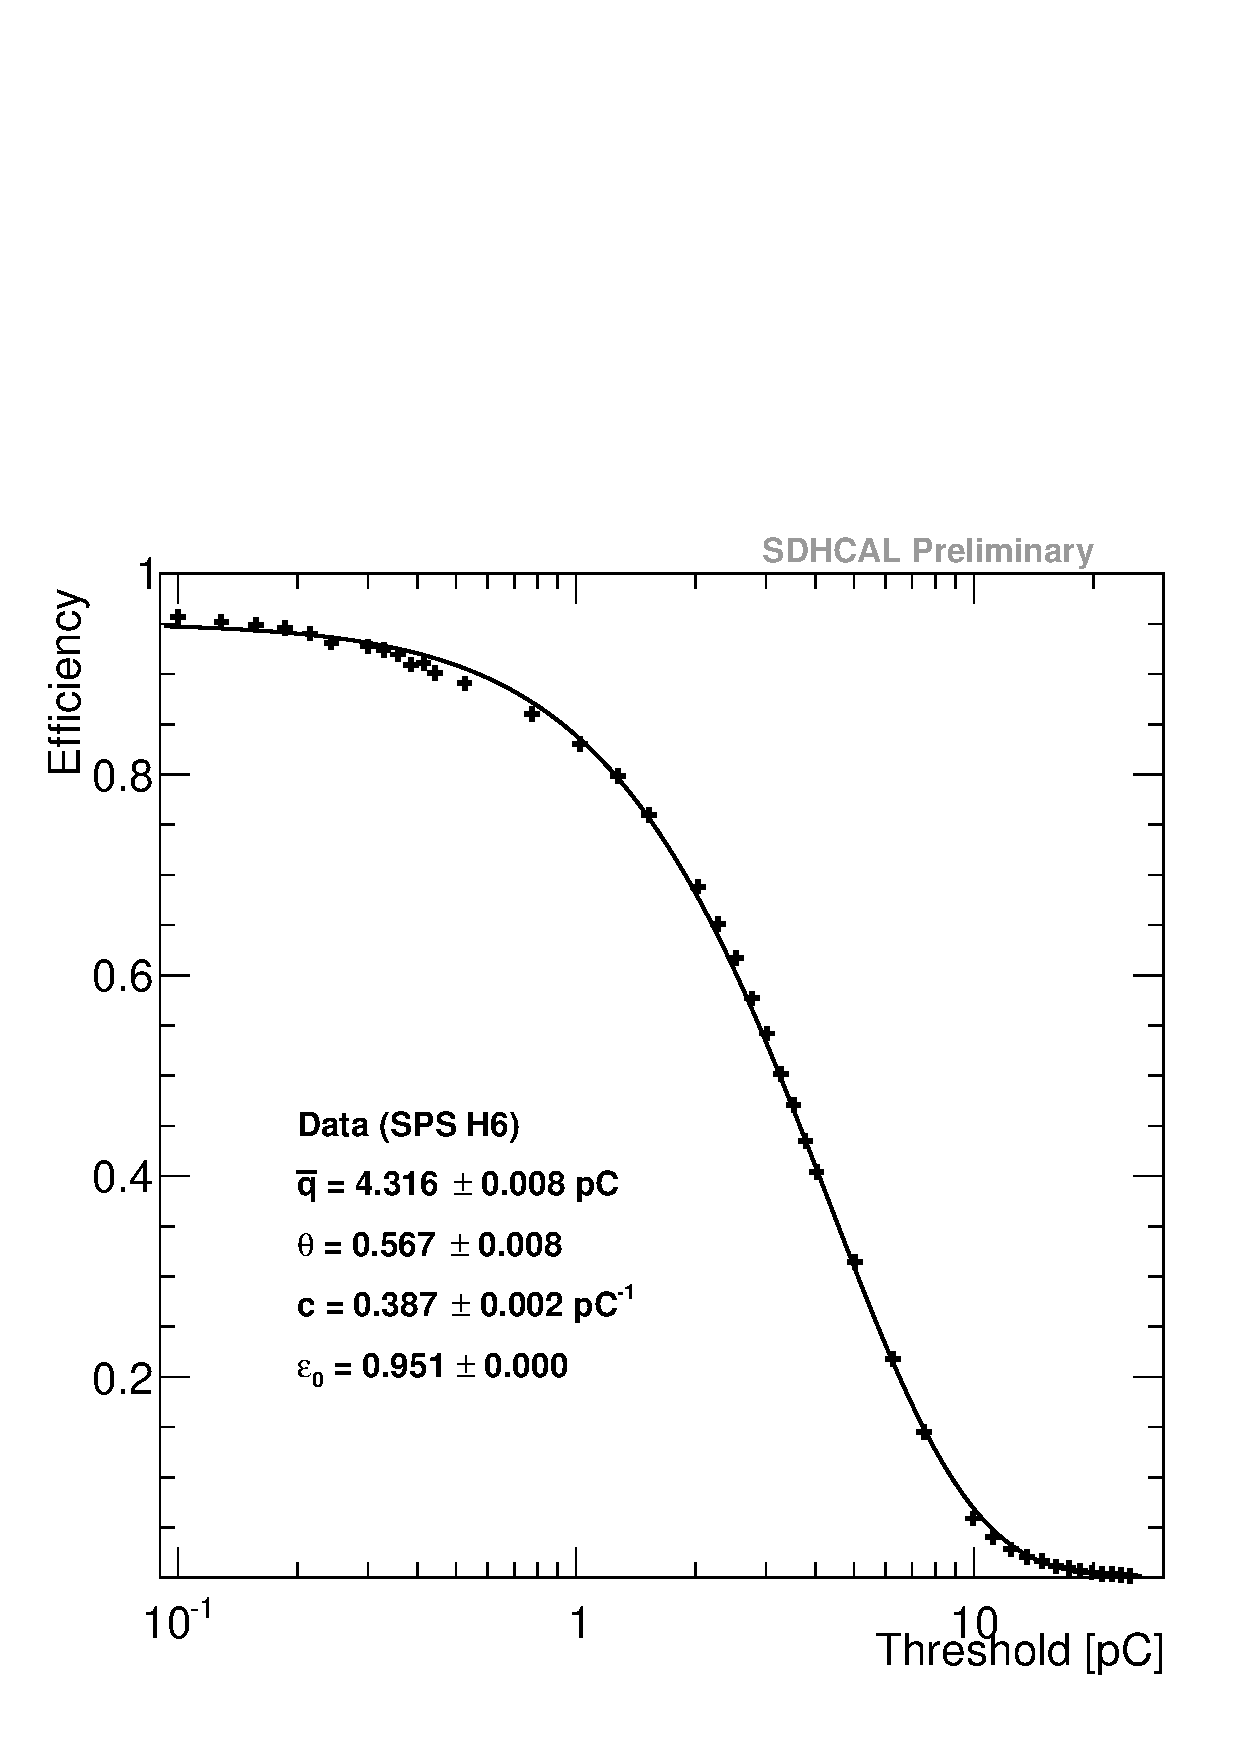
\includegraphics[width=.5\textwidth]{Digitizer/figs/thrScanDat.pdf}}
  \subfigure[]{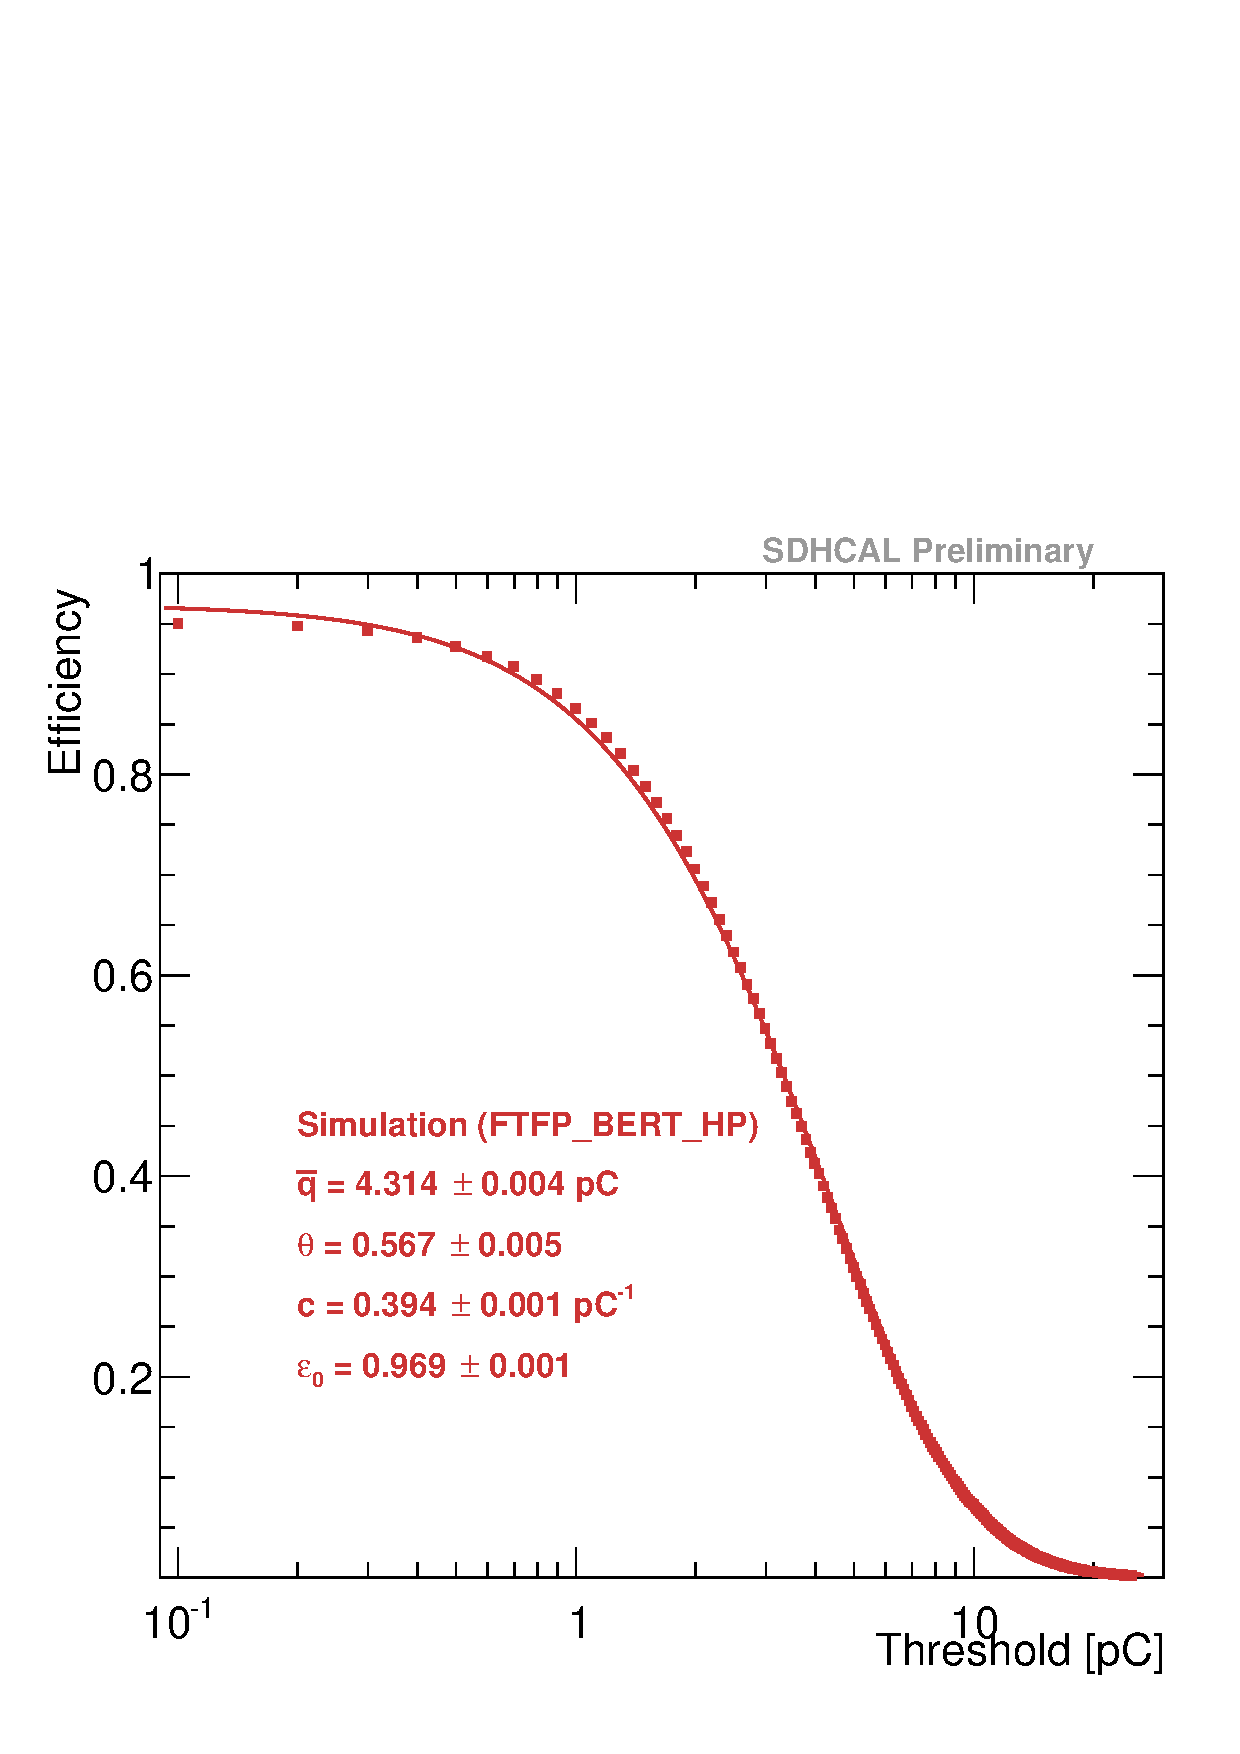
\includegraphics[width=.5\textwidth]{Digitizer/figs/thrScanSim.pdf}}
  \caption{Efficacité de détection en fonction des seuils en $pC$ pour les données (a) et pour la simulation (b). \label{fig.thrScan}}
\end{figure}
 La même procédure est réalisée avec la simulation. Les paramètres $\bar q$ et $\theta$ sont fixés dans l'algorithme SimDigital pour reproduire les résultats de l'ajustement obtenu avec les données du prototype. La figure~\ref{fig.thrScan}(b) montre la courbe d'efficacité moyenne en fonction du seuil pour la simulation. Le tableau~\ref{tab.inputPolya} présente les valeurs d'entrées des paramètres de la distribution de Polya utilisées dans l'algorithme.
\begin{table}[!ht]
  \begin{center}
    \begin{tabular}{c|c}
      \rowcolor{black!20!white}Paramètre & Valeur\\
      \rowcolor{black!5!white}\hline
      \rowcolor{black!5!white}$\bar q$ & $4.58 pC$\\
      \rowcolor{black!5!white}$\theta$ & $1.12$\\
    \end{tabular}
  \end{center}
  \caption{Valeurs d'entrées des paramètres de la distribution de Polya utilisée dans l'algorithme SimDigital.}
  \label{tab.inputPolya}
\end{table}
 Cependant, les valeurs des paramètres obtenues avec l'ajustement (cf. Eq.~\ref{eq.fitScan}) sont légèrement différentes des valeurs d'entrées. Ceci vient de l'étalement de la charge induite sur plusieurs canaux de lecture (cf. étape~\ref{it.spliting} de la section~\ref{sec.algo} de ce chapitre). Cet étalement fait qu'une fraction de la charge induite est perdue lorsque les seuils sont appliqués.
%%%%%%%%%%%%%%%%%%%%%%%%%%%%%%%%%%%%%

\subsubsection{Répartition de la charge}
Les paramètres introduits dans les équations~\ref{eq.ratio} et~\ref{eq.norm} sont réglés pour reproduire la multiplicité moyenne et le nombre de hits dans les gerbes électromagnétiques. La multiplicité moyenne pour chaque GRPC est calculée en utilisant la même méthode de reconstruction de trace décrite dans la chapitre~\ref{chap.sdhcal}. De nombreuses configurations de ces paramètres ont été testées pour reproduire à la fois la multiplicité moyenne et le nombre de hits dans les gerbes électromagnétiques. Le paramètre $n$ de l'équation~\ref{eq.ratio} est fixé à~2. Il n'était pas possible de reproduire les différentes observables des données avec $n=1$. Une augmentation de la valeur de ce paramètre n'apporte pas d'amélioration et ajoute des difficultés pour paramétrer l'algorithme. Le tableau~\ref{tab.splitting} présente les valeurs d'entrées des paramètres $\alpha$ et $\sigma$.
\begin{table}[!ht]
  \begin{center}
    \begin{tabular}{c|c}
      \rowcolor{black!20!white}Paramètre & Valeur\\
      \rowcolor{black!5!white}\hline
      \rowcolor{black!5!white}$\alpha_0$ & $1.0$\\
      \rowcolor{black!5!white}$\sigma_0$ & $1.0~mm$\\
      \rowcolor{black!5!white}$\alpha_1$ & $0.00083$\\
      \rowcolor{black!5!white}$\sigma_1$ & $9.7~mm$\\
    \end{tabular}
  \end{center}
  \caption{Valeurs d'entrées des paramètres introduits dans l'équation~\ref{eq.ratio}.}
  \label{tab.splitting}
\end{table}
Le paramètre $r_{max}$ est fixé à 30 $mm$. Une augmentation de cette valeur n’entraîne pas de variation significative sur le résultat final de la simulation. En effet, la quantité de charge déposée sur les carreaux éloignés de plus de 30 $mm$ de la particule est négligeable (avec le paramétrage actuel). La figure~\ref{fig.eff_mul_layer} montre l'efficacité (figure~\ref{fig.eff_mul_layer}(a)) et la multiplicité (figure~\ref{fig.eff_mul_layer}(b)) moyenne par chambre pour les données et la simulation.
\begin{figure}[!ht]
  \subfigure[]{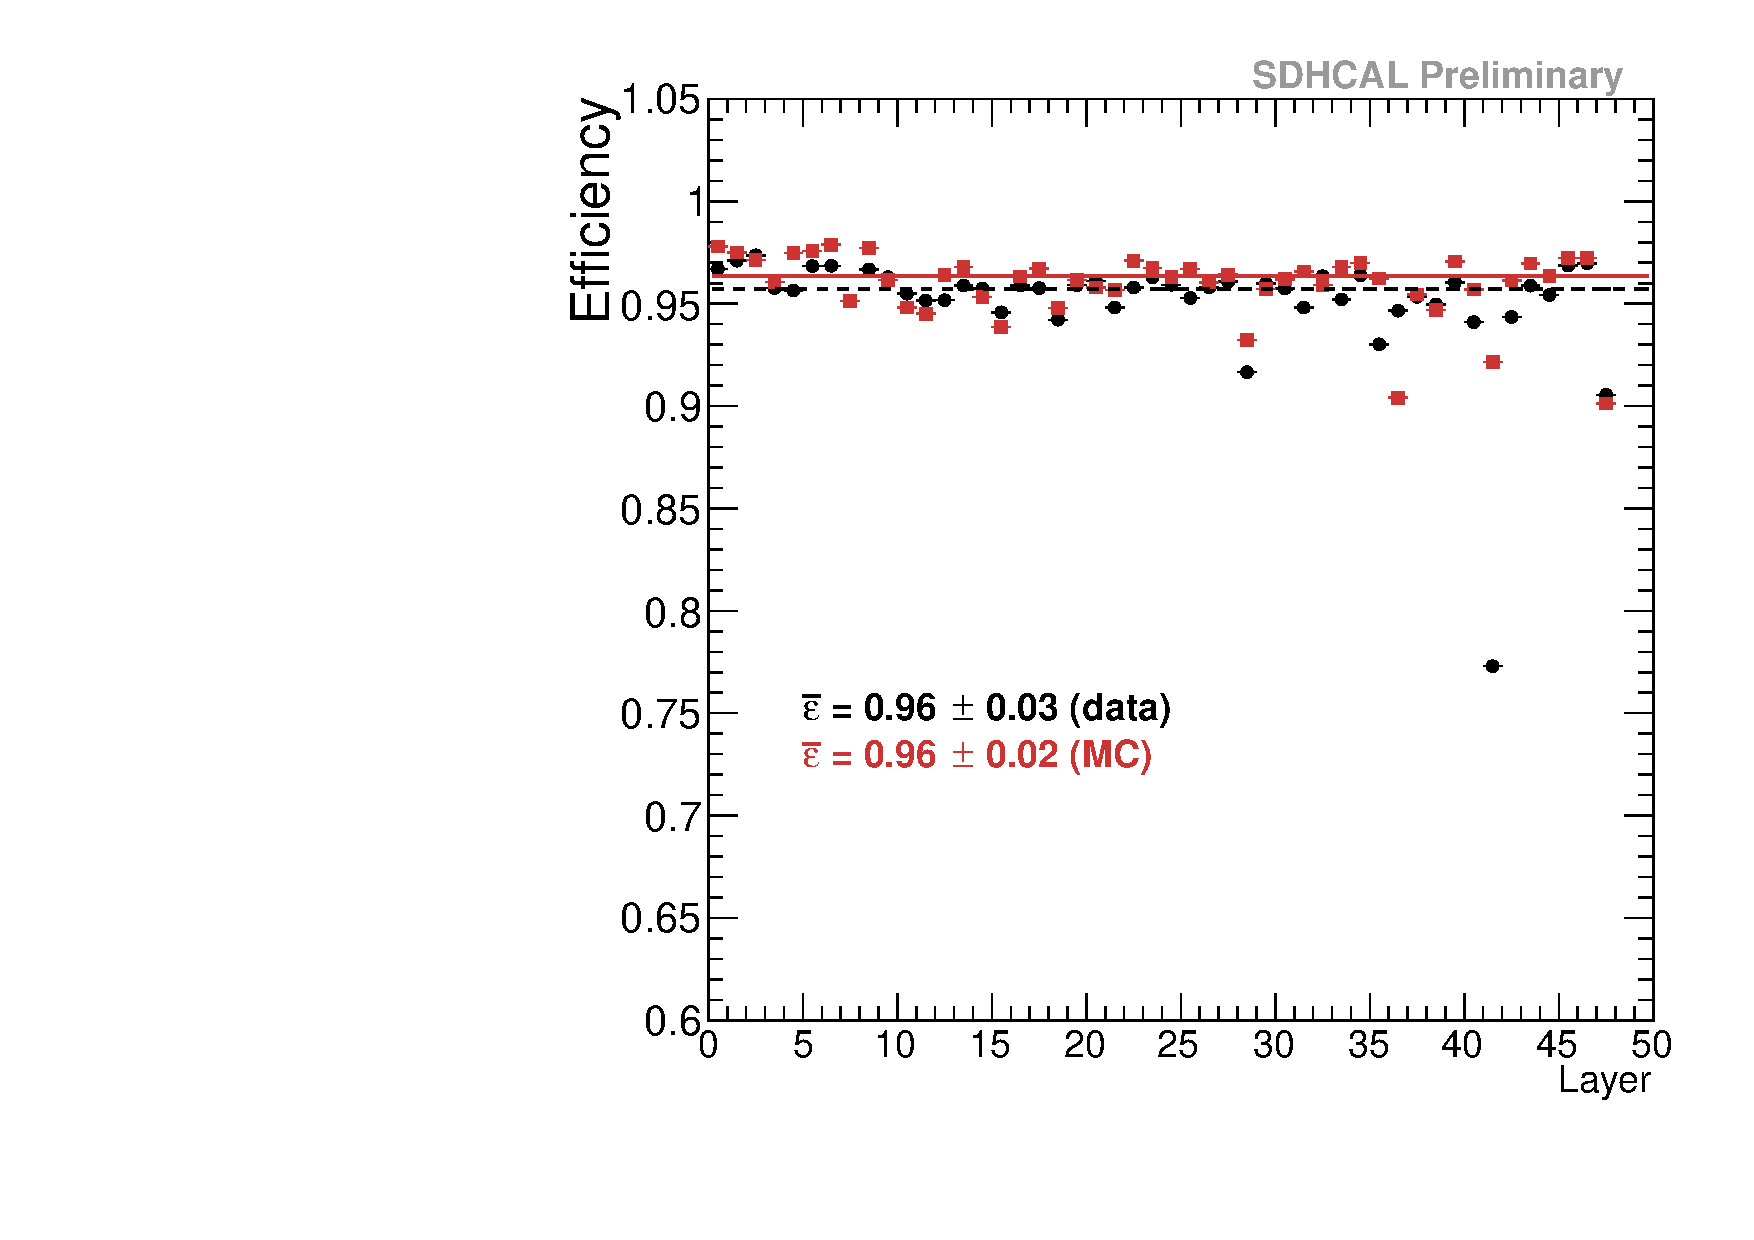
\includegraphics[width=.5\textwidth]{Digitizer/figs/effLayer.pdf}}
  \subfigure[]{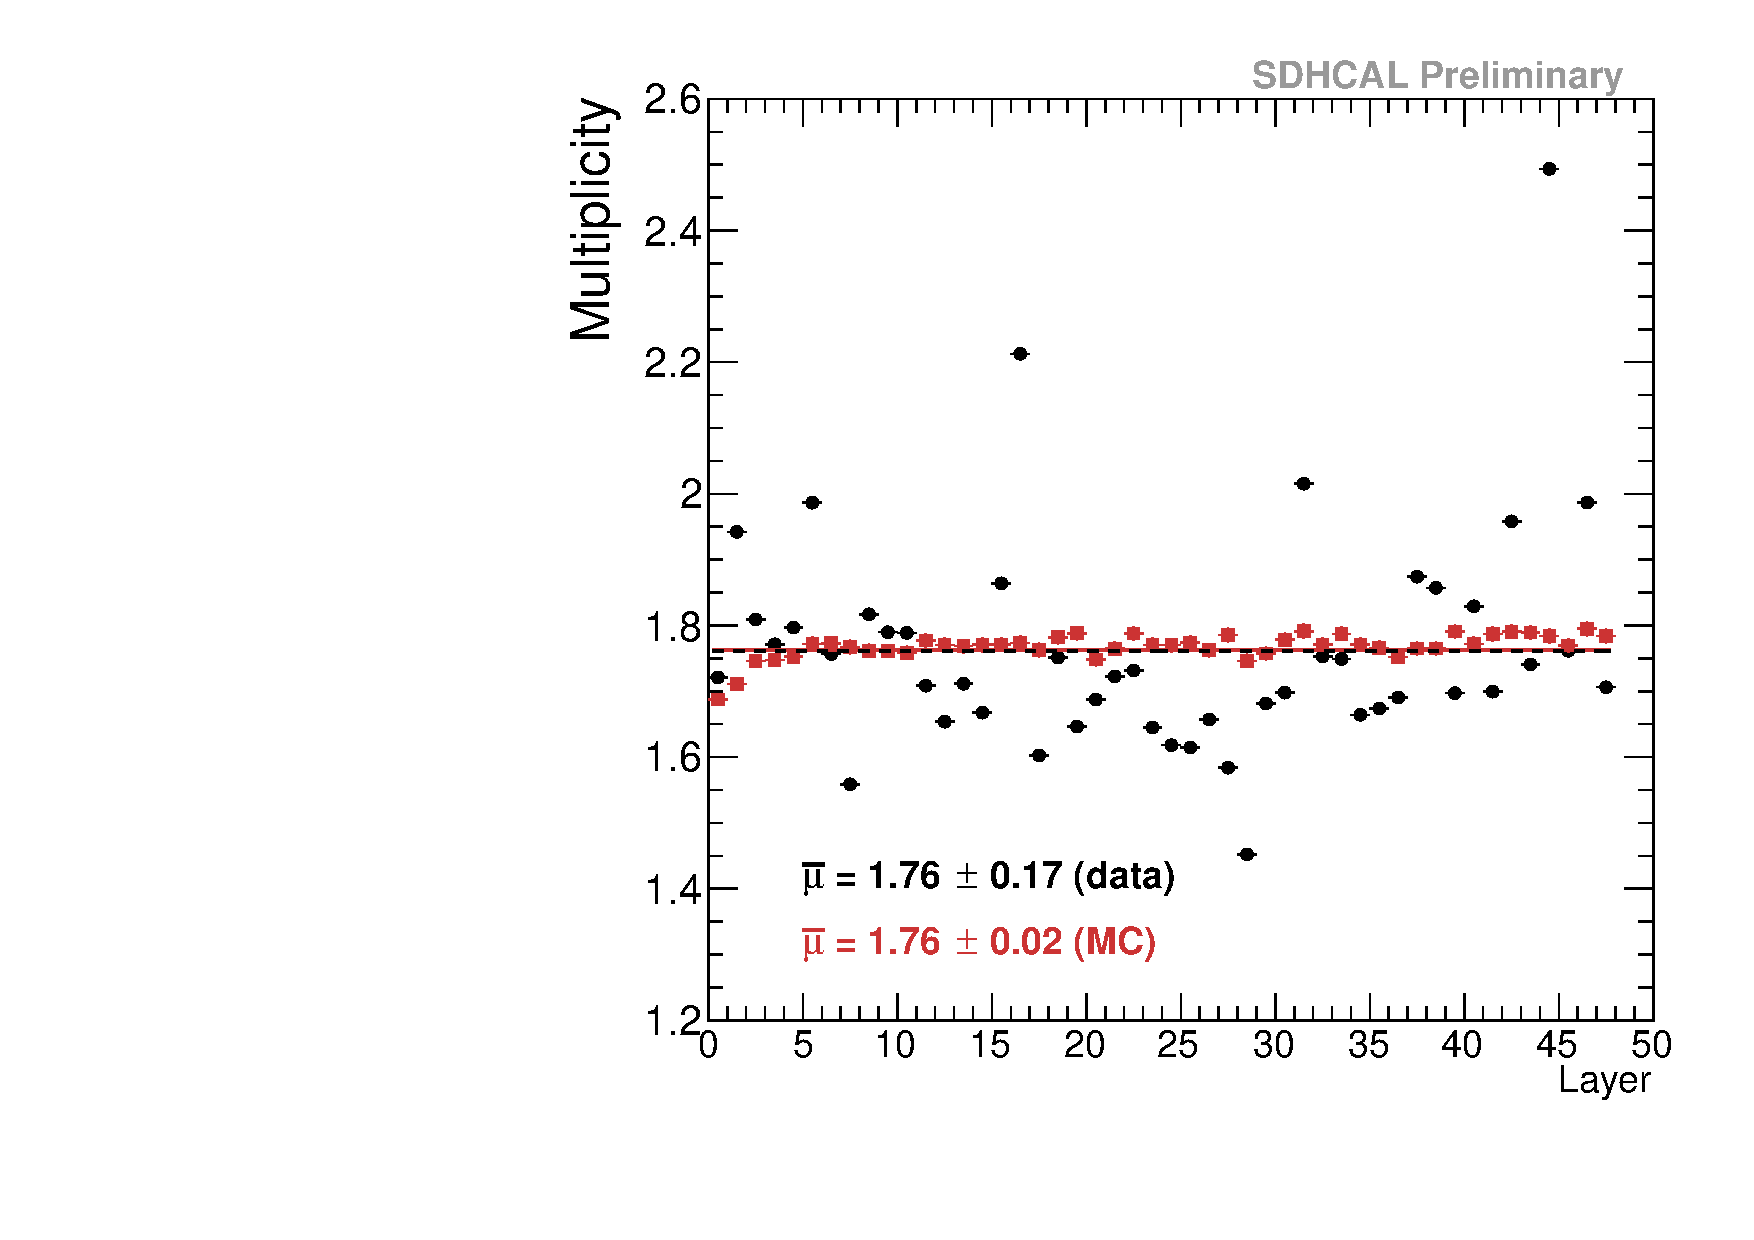
\includegraphics[width=.5\textwidth]{Digitizer/figs/mulLayer.pdf}}
  \caption{Efficacité moyenne (a) et multiplicité moyenne (b) par plan. Les données sont représentées par des cercles noirs et la simulation par des carrés rouges.\label{fig.eff_mul_layer}}
\end{figure}
L'efficacité dans la simulation suit raisonnablement bien les fluctuations des données car les cartes d'efficacité (déterminées avec les données) sont utilisées par l'algorithme. En revanche, les fluctuations de la multiplicité ne sont pas reproduites par la simulation. Les différences de multiplicité d'une chambre à l'autre peuvent s'expliquer par des différences de résistivité de la peinture appliquée sur les verres et par des imperfections de la géométrie des détecteurs. De plus, lors des tests en faisceaux de 2015 au PS au CERN, l'étude de scan en seuil a de nouveau été réalisée. Cette fois, nous avons fait varier les seuils dans toutes les chambres. Ainsi, les paramètres d'une distribution de Polya peuvent être extraits pour chaque détecteur. La figure~\ref{fig.polya_ps_2015} montre l'efficacité de détection de deux GRPC du prototype en fonction du seuil. Ces efficacités sont aussi ajustées avec la fonction~\ref{eq.fitScan}.
\begin{figure}[!ht]
  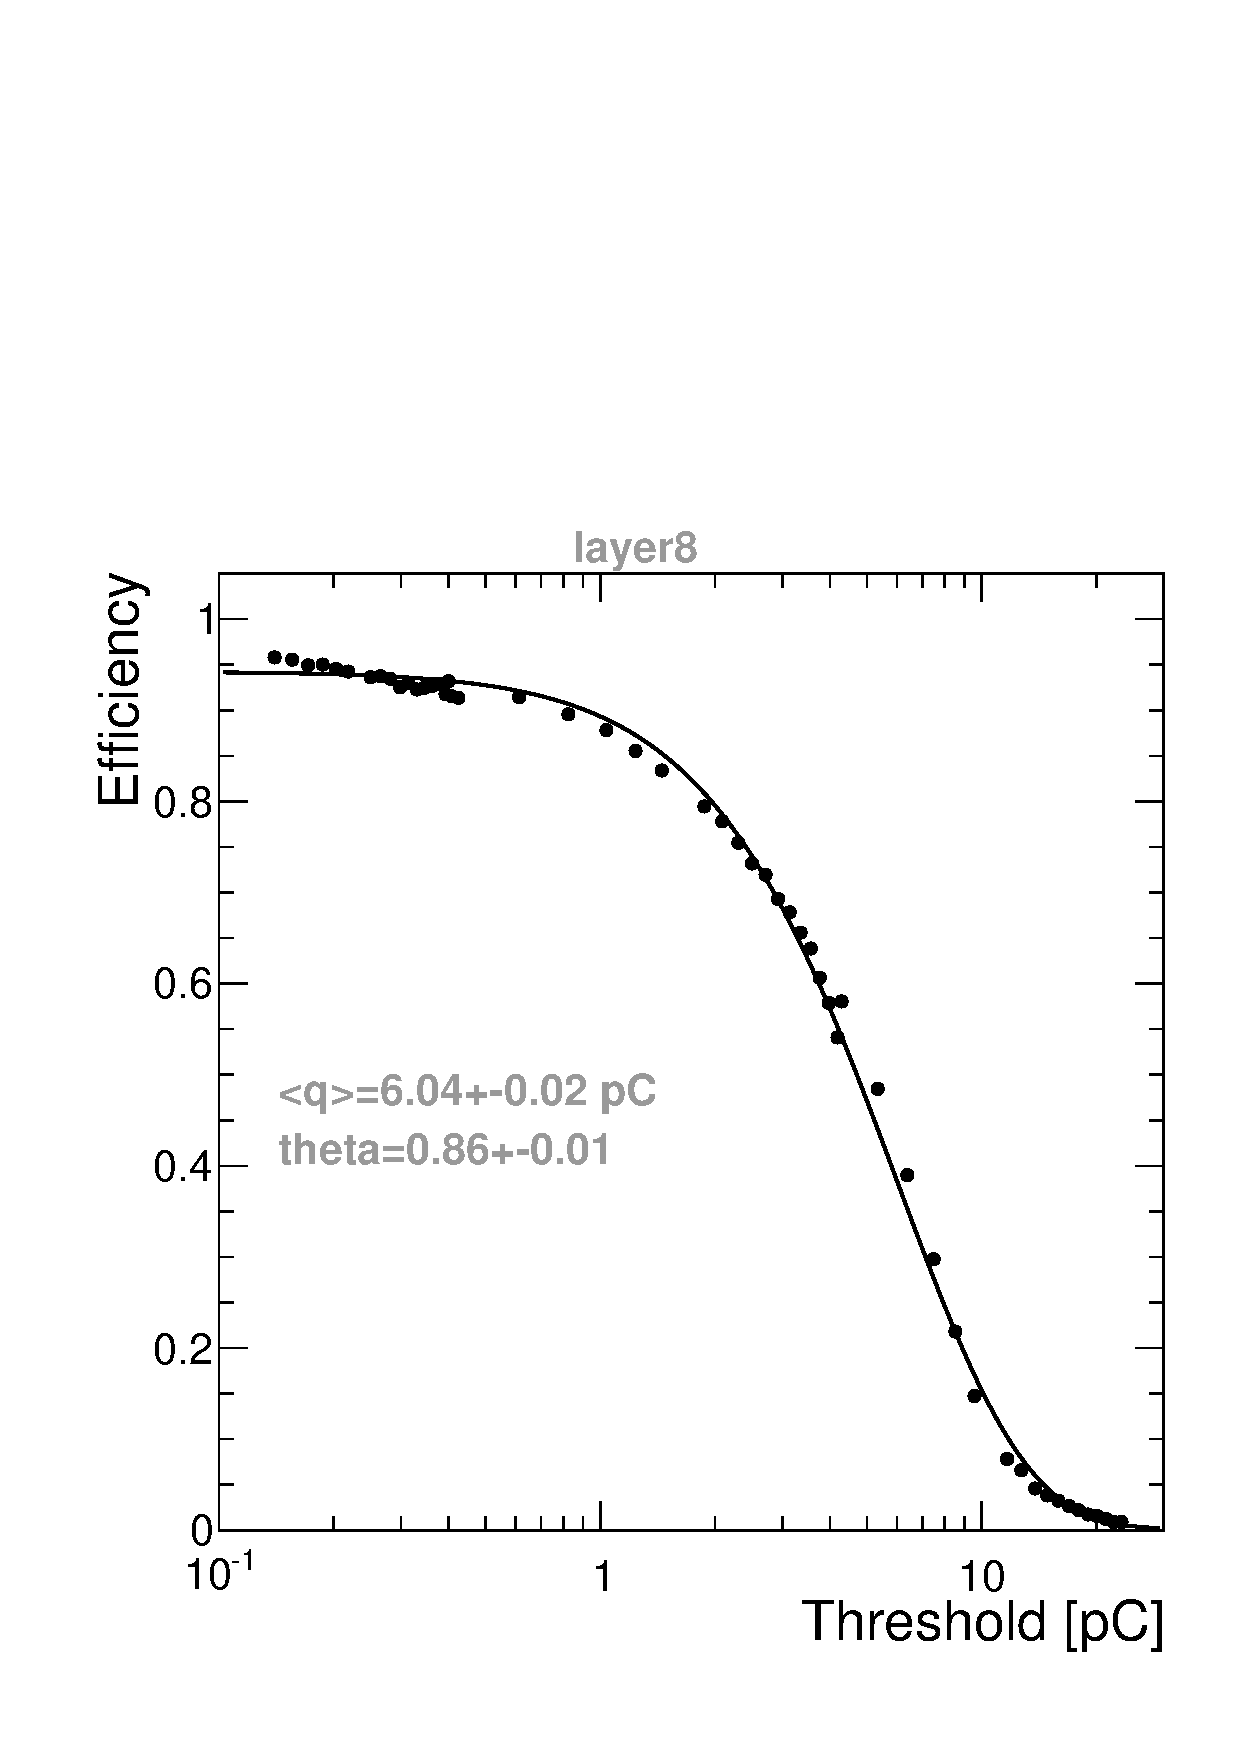
\includegraphics[width=.5\textwidth]{Digitizer/figs/layer8.pdf}
  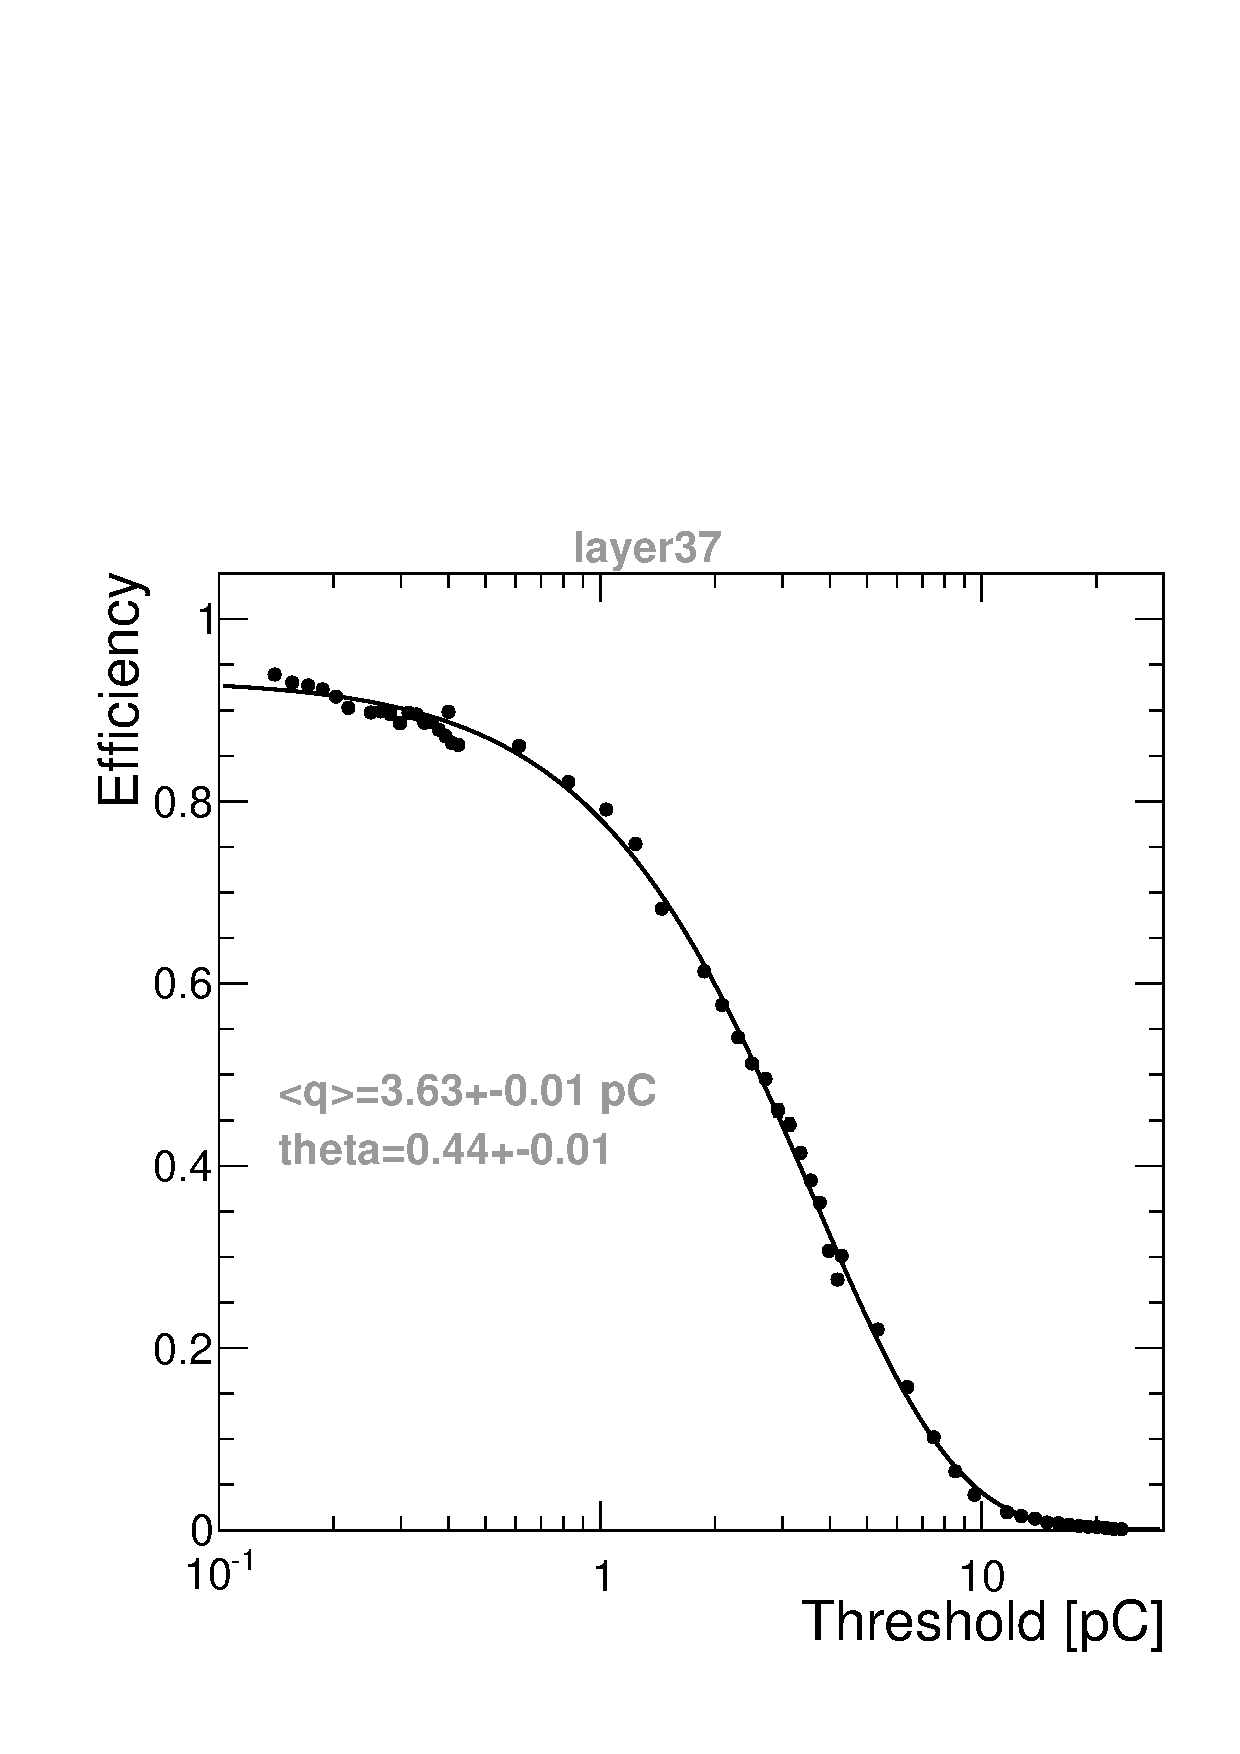
\includegraphics[width=.5\textwidth]{Digitizer/figs/layer37.pdf}
  \caption{Exemple d'efficacité en fonction du seuil pour deux chambres du prototype.}
  \label{fig.polya_ps_2015}
\end{figure}
Les paramètres de la distribution de Polya, indiqués sur ces deux figures, sont très différents. Le tableau~\ref{tab.polya_params_48} présente les valeurs moyennes et les écarts types des paramètres $\bar q$ et $\theta$ des distributions de Polya des 48 chambres du prototype SDHCAL.
\begin{table}[!ht]
  \begin{center}
    \begin{tabular}{c|c|c}
      \rowcolor{black!20!white}Paramètre & Valeur moyenne & Ecart type\\
      \rowcolor{black!5!white}\hline
      \rowcolor{black!5!white}$\bar q$ & $5.33\pm0.17~pC$ & $1.21\pm0.25~pC$\\
      \rowcolor{black!5!white}$\theta$ & $0.90\pm0.05$ & $0.33\pm0.07$\\
    \end{tabular}
  \end{center}
  \caption{Valeur moyenne et écart type des paramètres $\bar q$ et $\theta$ des distributions de Polya des 48 chambres du prototype SDHCAL.}
  \label{tab.polya_params_48}
\end{table}
L'utilisation d'une distribution de Polya différente pour chaque chambre devrait permettre à la multiplicité simulée de mieux reproduire les fluctuations des données expérimentales.
%%%%%%%%%%%%%%%%%%%%%%%%%%%%%%%%%%%%%

\subsubsection{Dépendance de l'angle d'incidence}
Lors des tests sur faisceau, les muons incidents sont, pour la plupart, perpendiculaires au détecteur. Cependant, dans les gerbes hadroniques et électromagnétiques des particules secondaires sont émises avec des angles différents. Une étude de la multiplicité avec des particules cosmiques est alors nécessaire pour déterminer et simuler la réponse d'une GRPC sur une large gamme d'angles d'incidences. La figure~\ref{fig.mul_vs_theta}(a) montre la multiplicité en fonction de $cos{\theta}$ où $\theta$ est l'angle entre la normale au détecteur (axe $(0z)$ pour le prototype) et la particule incidente. Cette figure montre que la multiplicité pour les données expérimentales, augmente avec l'angle de la particule incidente alors qu'elle est plus plate pour la simulation. Une correction de la charge simulée est nécessaire pour reproduire le comportement des données. Une correction utilisant l'équation~\ref{eq.lengthcorrection} est préférée à une correction utilisant "$\frac{1}{cos\theta'}$" (avec $\theta'$ l'angle entre le segment et la normale au détecteur) car cette dernière peut générer des charges simulées infinies. 
\begin{figure}[!ht]
  \subfigure[]{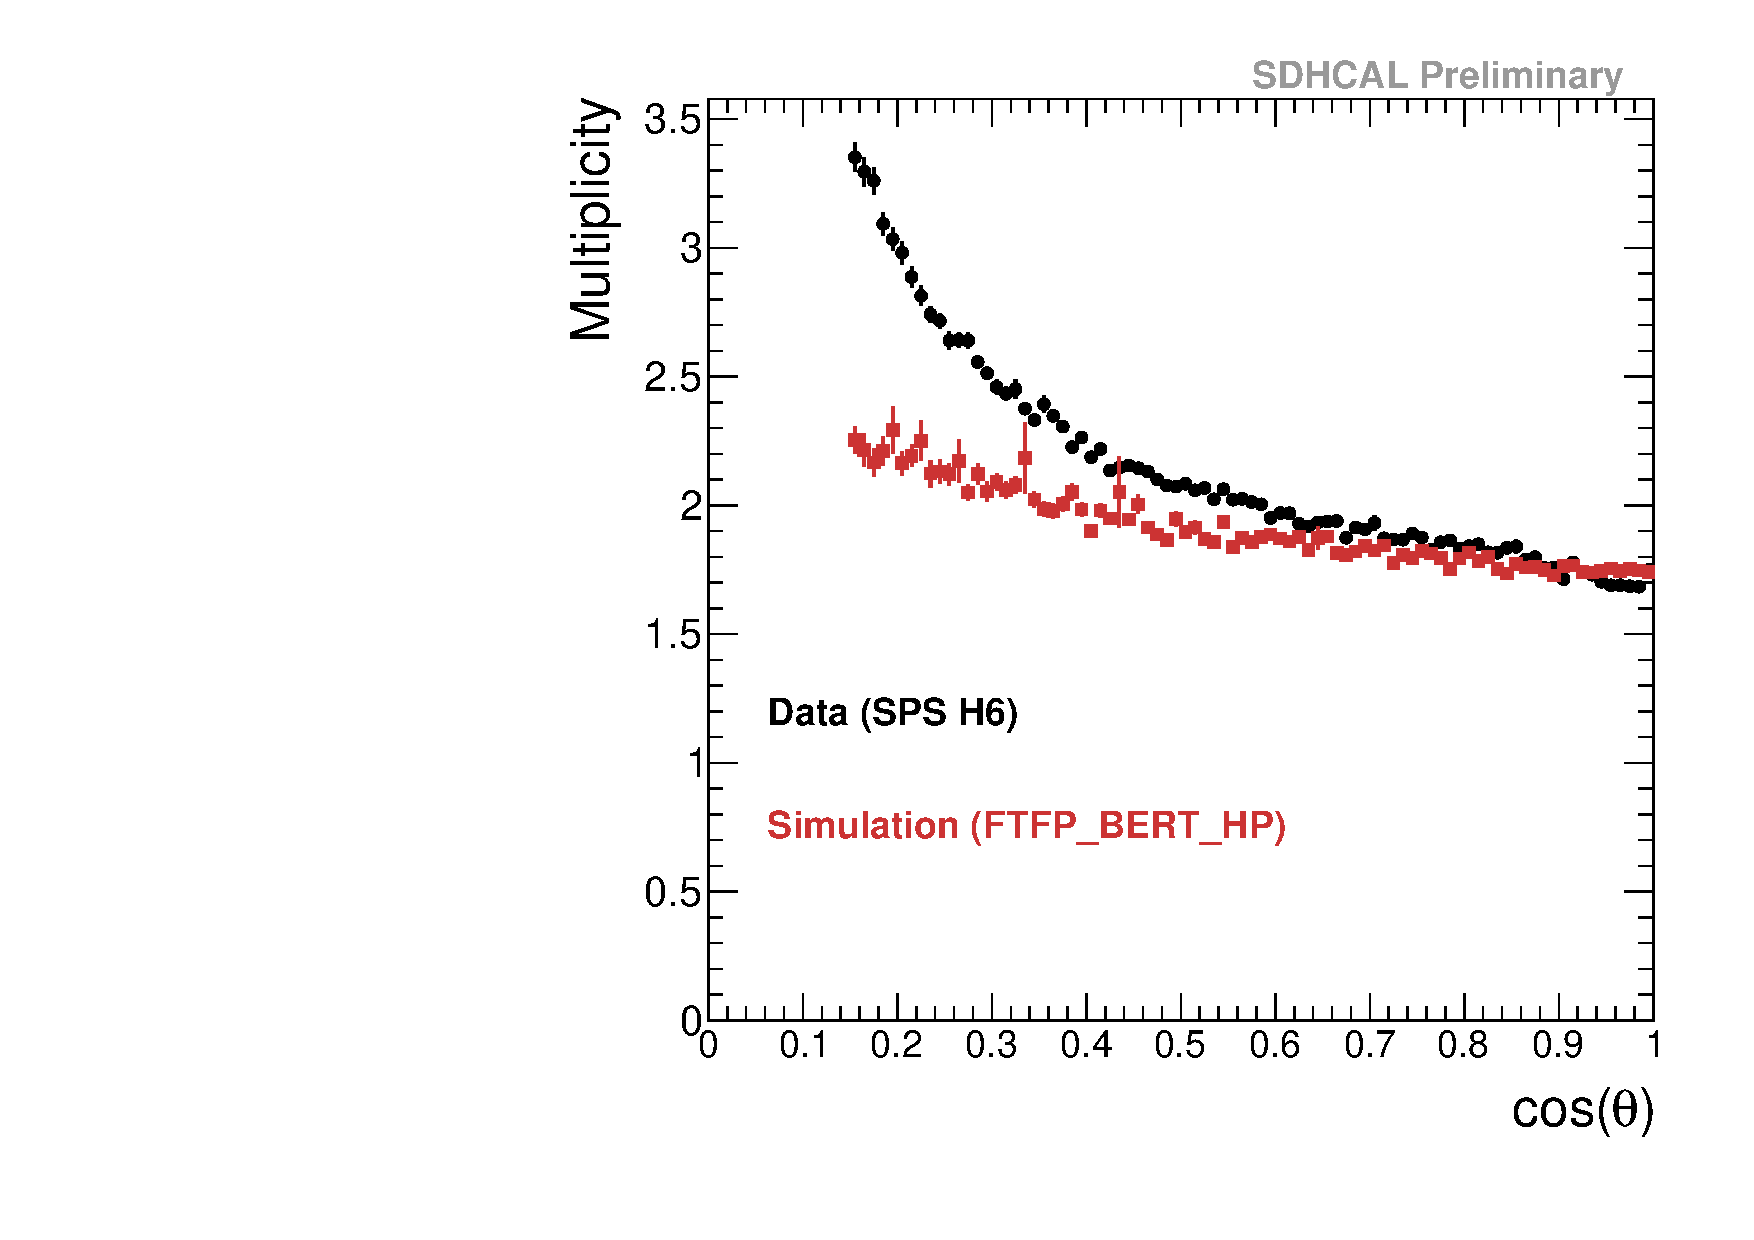
\includegraphics[width=.5\textwidth]{Digitizer/figs/mul_vs_thetaNLC.pdf}}
  \subfigure[]{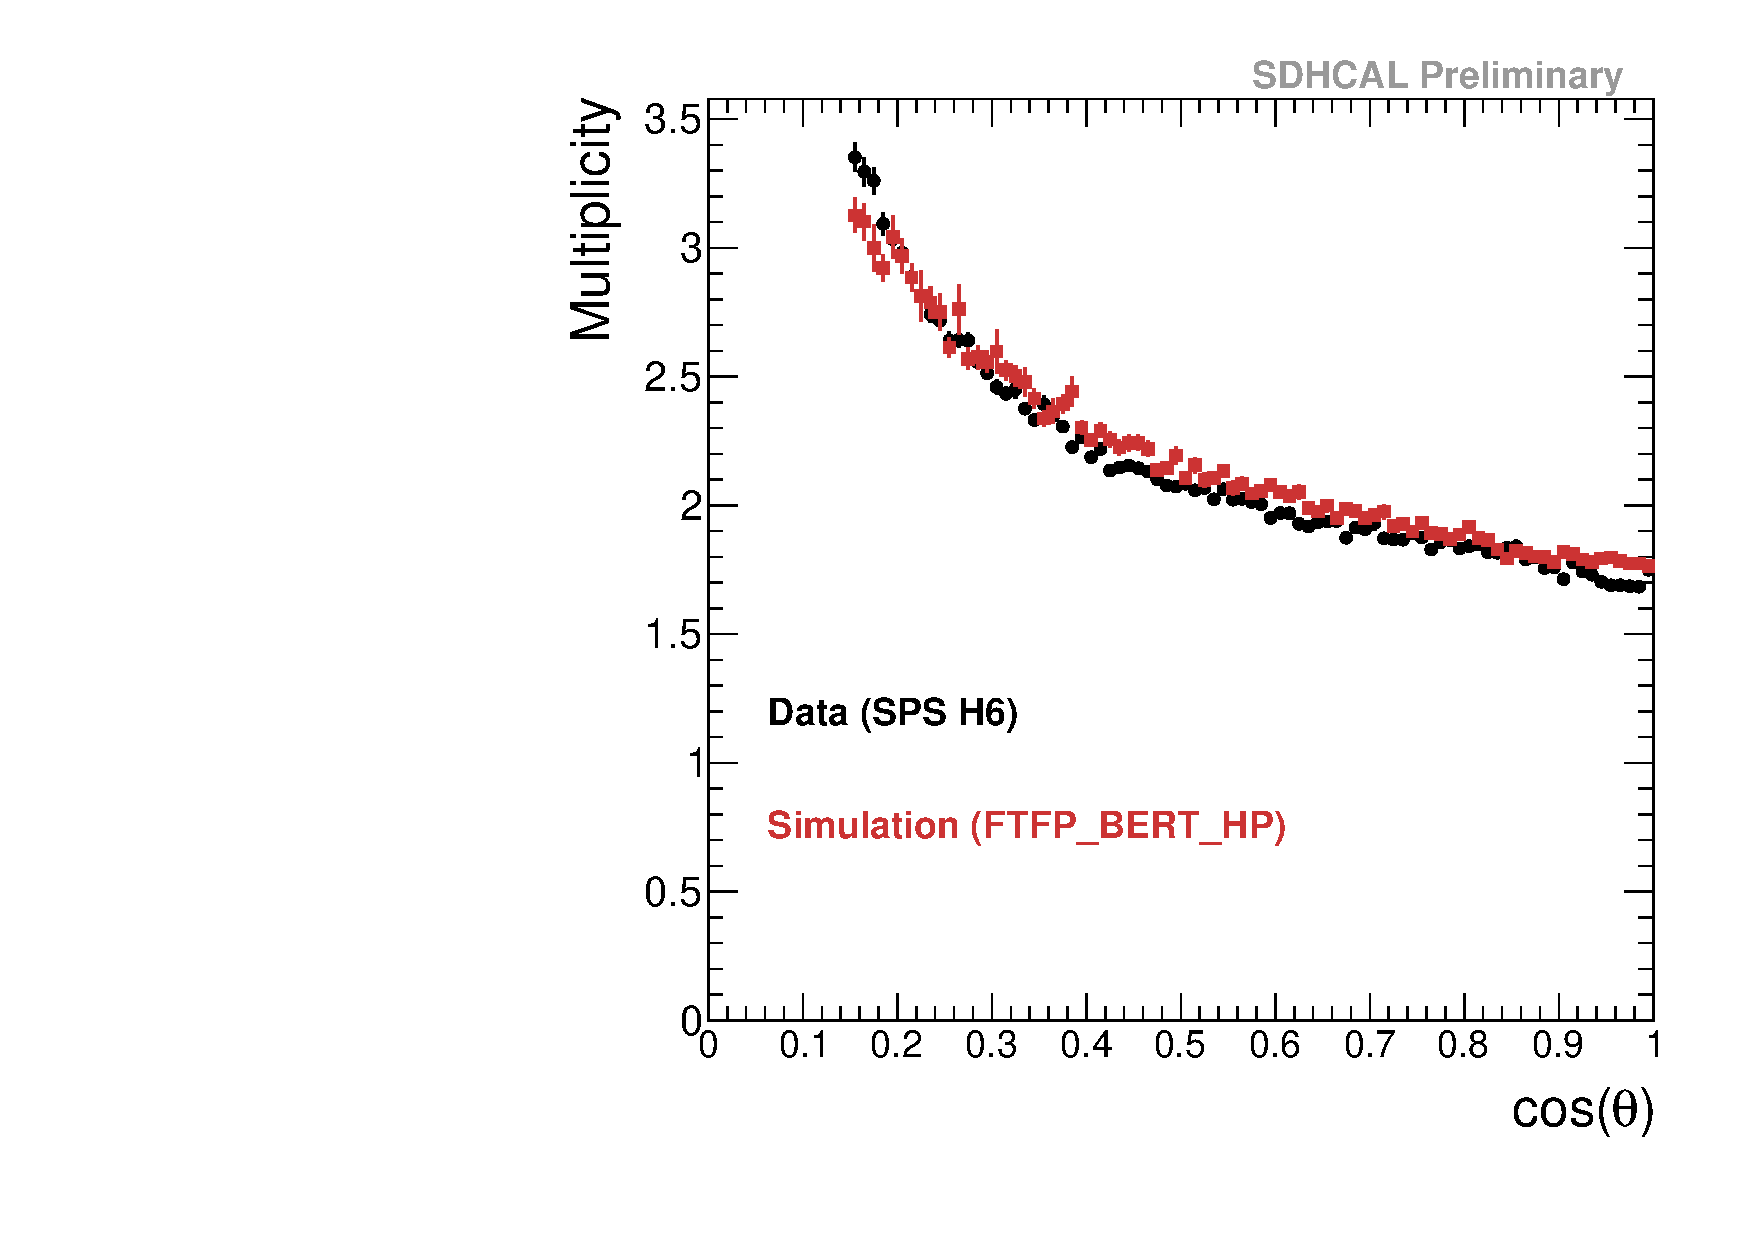
\includegraphics[width=.5\textwidth]{Digitizer/figs/mul_vs_theta.pdf}}
  \caption{Multiplicité moyenne en fonction de $cos\theta$ avec des cercles noirs pour les donées et des carrés rouges pour la simulation. (a): sans correction sur la longueur des segments; (b): avec correction sur la longueur des segments. \label{fig.mul_vs_theta}}
\end{figure}
La figure~\ref{fig.mul_vs_theta}(b) montre un bon accord entre les données et la simulation pour la multiplicité en fonction de $cos\theta$ après l'application de cette correction. La valeur du facteur $\kappa$ est optimisée pour reproduire les données et fixée à 0.40.
%% \begin{figure}[!ht]
%%   \begin{center}
%%     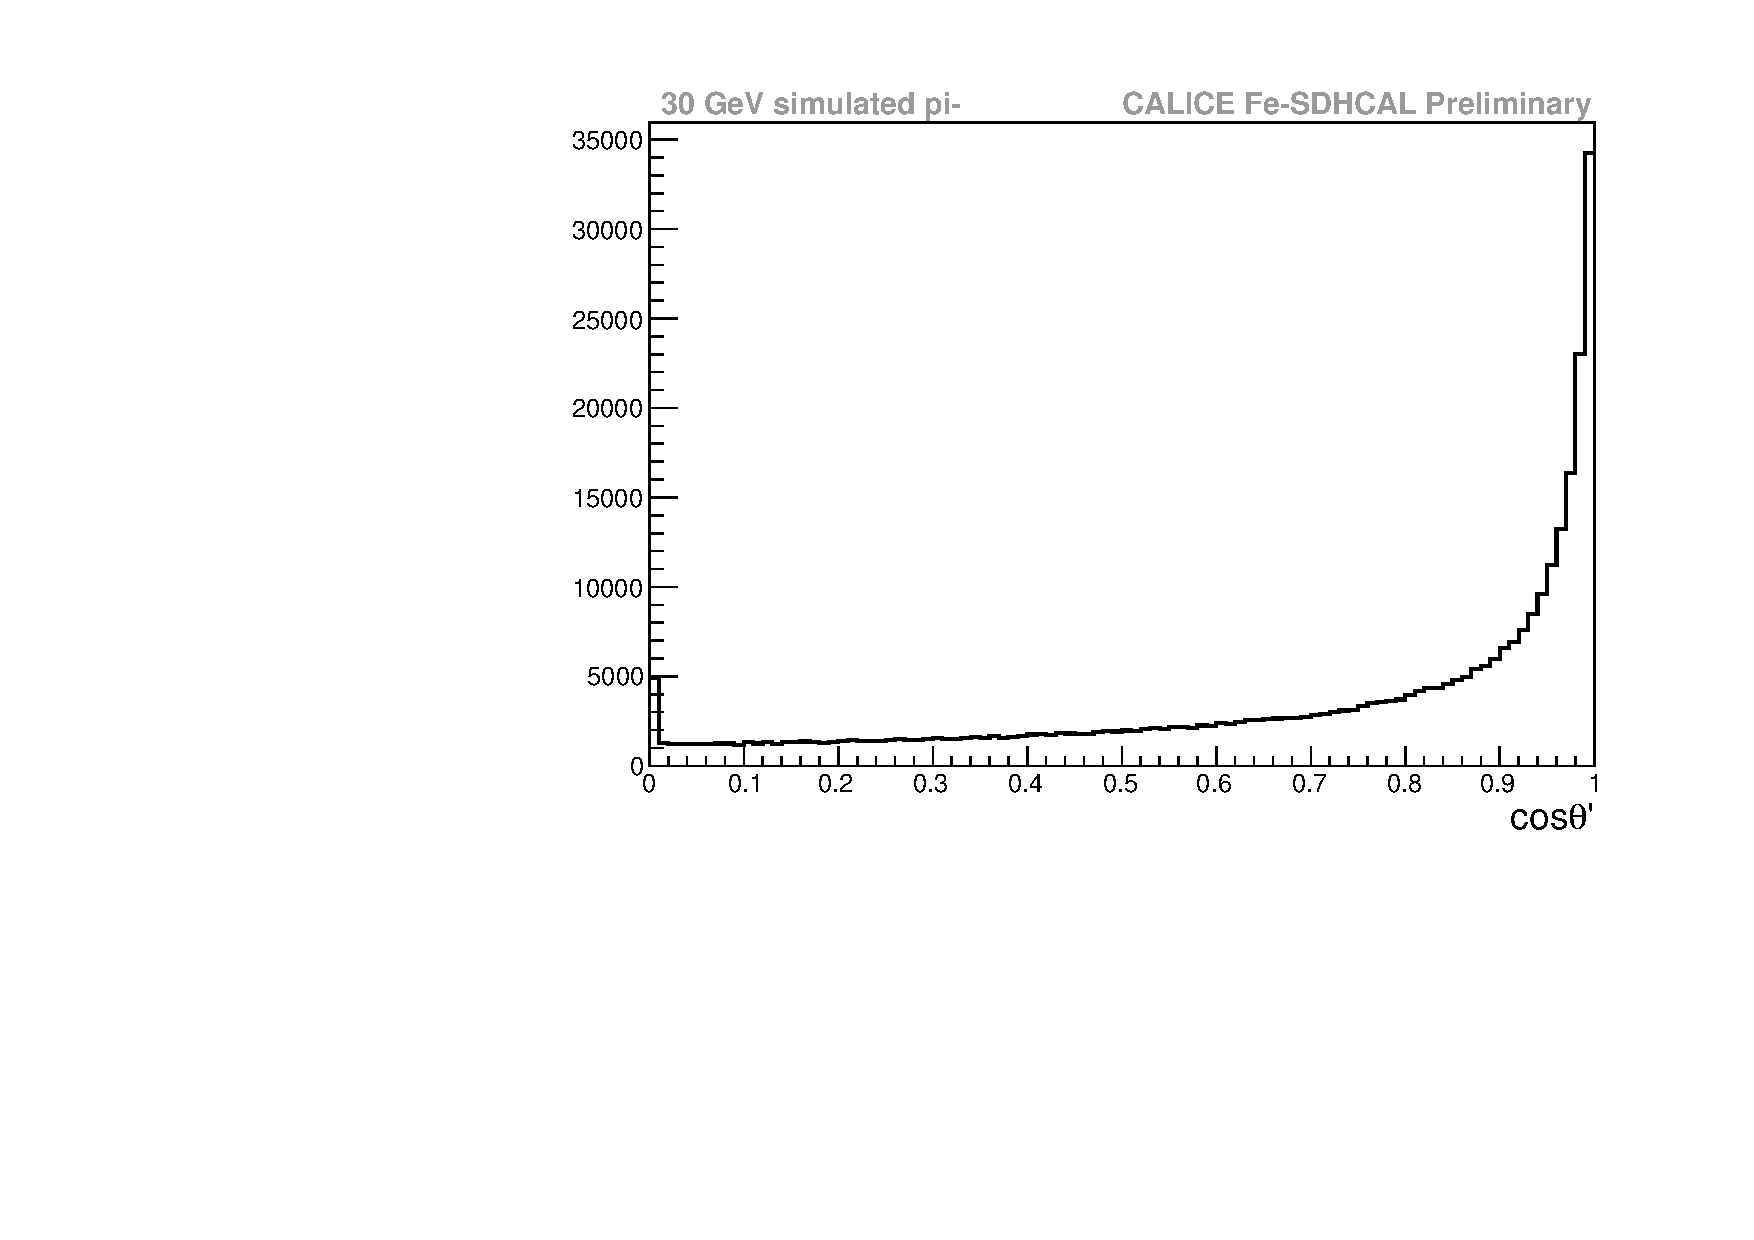
\includegraphics[width=.8\textwidth]{Digitizer/figs/costhetaPI30.pdf}
%%     \caption{Distribution du cos de l'angle de la step avec la normal à la GRPC pour une simulation d'un échantillon de pion à 30 GeV.}
%%     \label{fig.g4list}
%%   \end{center}
%% \end{figure}

%%%%%%%%%%%%%%%%%%%%%%%%%%%%%%%%%%%%%

\subsubsection{Paramétrage des seuils}
Nous avons vu dans la section~\ref{sec.sdhcal_thr} du chapitre~\ref{chap.sdhcal} comment les seuils sont réglés dans le prototype. Cependant comme ces travaux n'ont pas pu être effectués avec des détecteurs complets, il est probable que les valeurs de conversion (entre DAC et valeurs de seuil en $pC$) soient légèrement différentes pour le prototype. Ceci donne un peu de liberté pour régler les seuils dans la simulation. Les études de scan en seuil (cf. figures~\ref{fig.thrScan}(b)) montre qu'une faible variation du premier seuil ($seuil\in[0.1,0.4]~pC$) a des conséquences négligeables sur l'efficacité ($\varepsilon\in[0.94,0.95]$). Ainsi, la valeur du premier seuil utilisée dans la simulation est fixé à 0.114 $pC$ comme pour le prototype. Pour régler la valeur des seuils supérieurs, nous avons de nouveau réalisé une étude d'efficacité. La même méthode décrite dans le chapitre~\ref{chap.sdhcal} est utilisée pour déterminer si un plan est efficace. Lorsqu'un plan est efficace, il est aussi considéré comme efficace pour les seuils 2 et/ou 3 si au moins une cellule ayant une charge qui a passé ces seuils, est trouvée dans l'amas de cellules associées. Les seuils 2 et 3 sont alors réglés pour reproduire les efficacités des données expérimentales. 
\begin{figure}[!ht]
  \subfigure[]{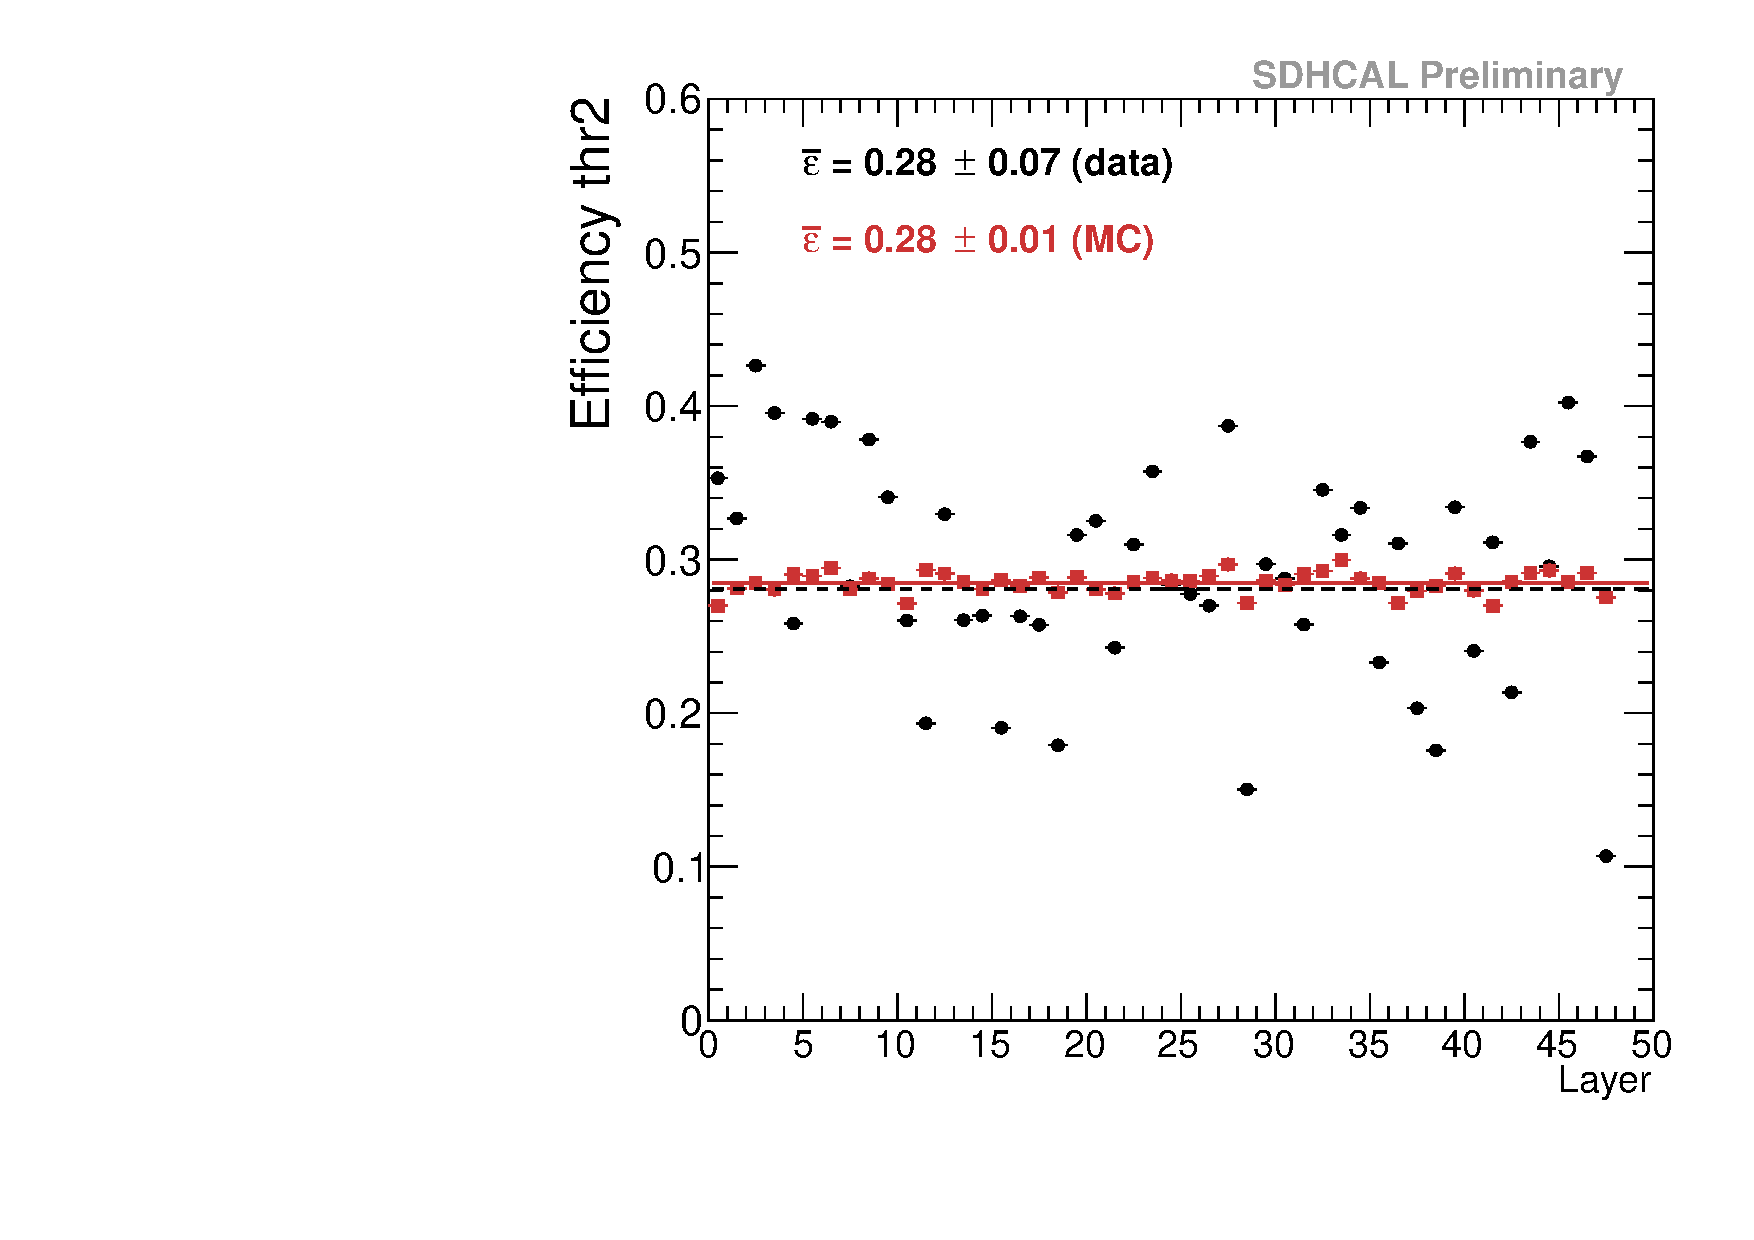
\includegraphics[width=.5\textwidth]{Digitizer/figs/eff2Layer.pdf}}
  \subfigure[]{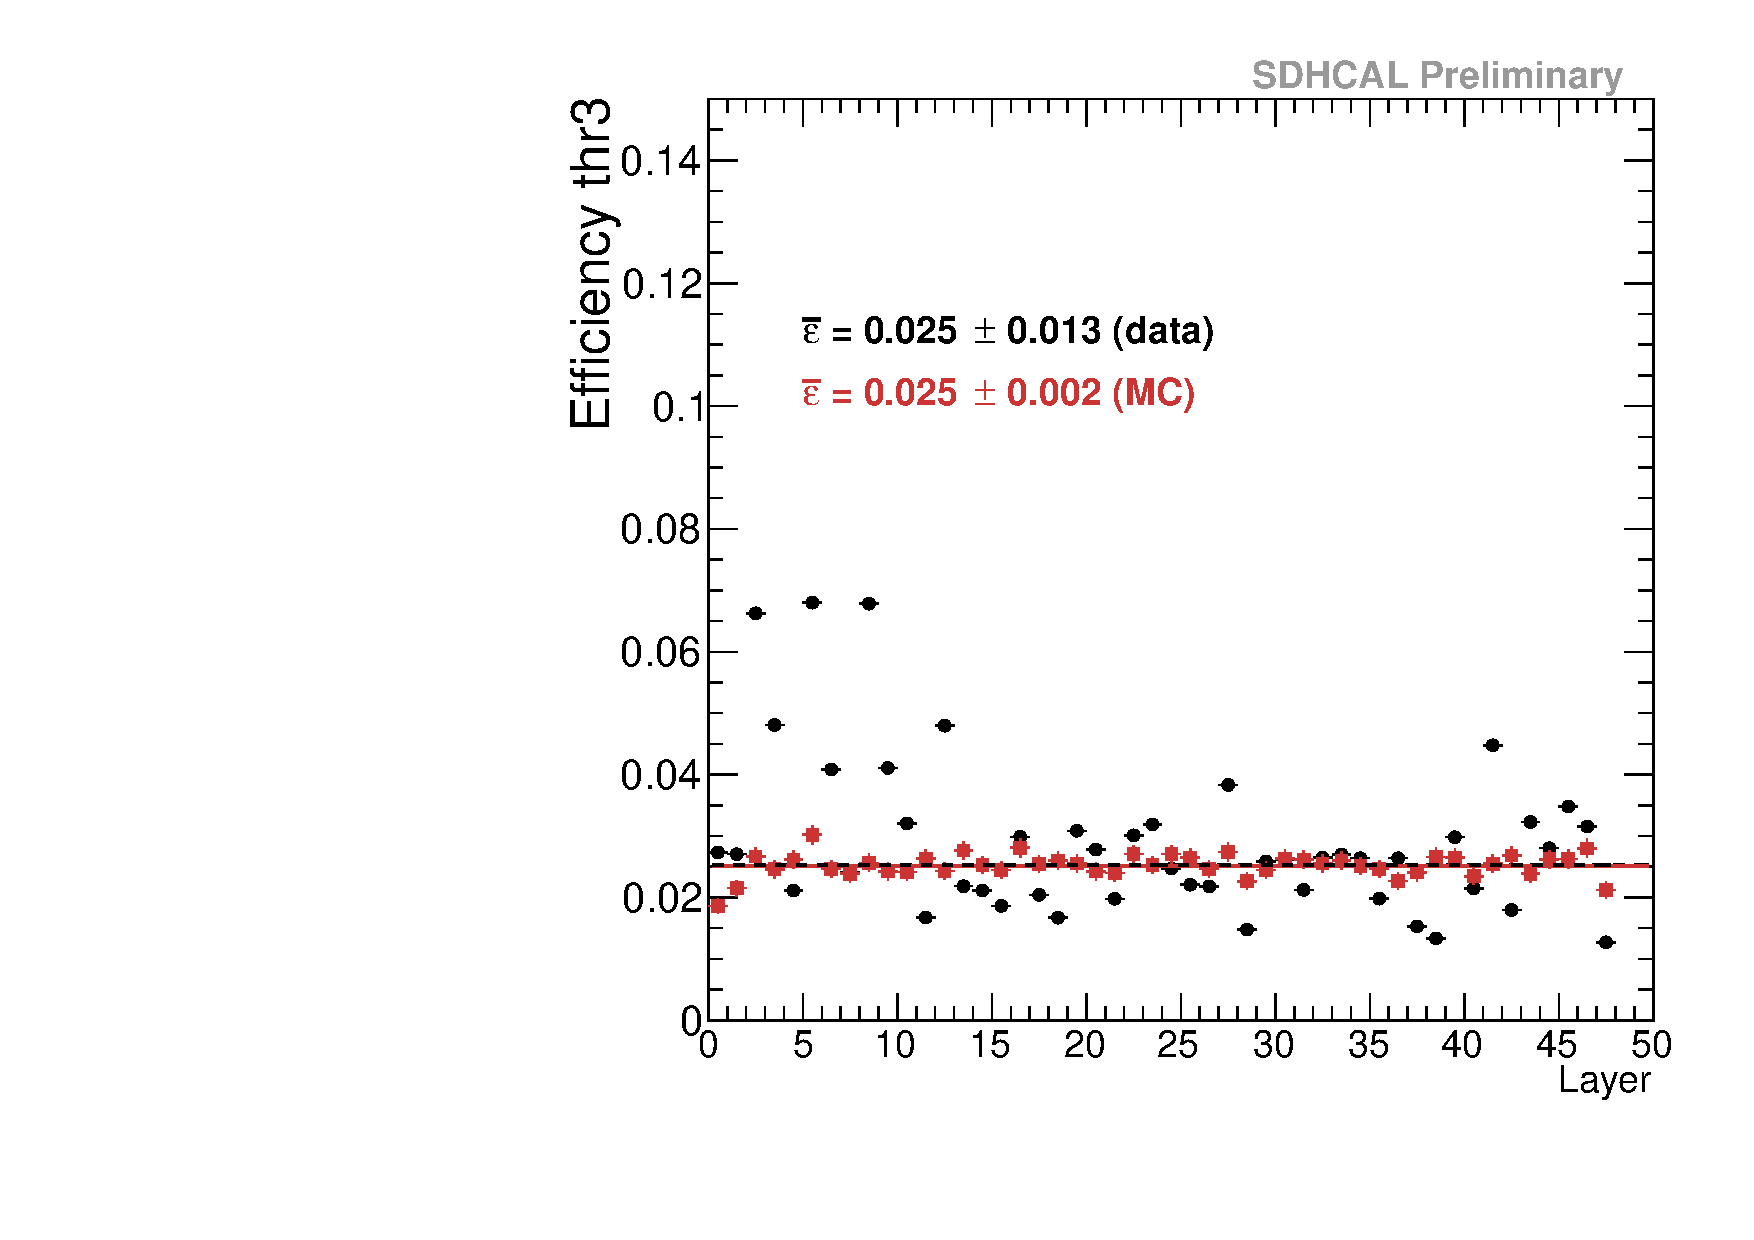
\includegraphics[width=.5\textwidth]{Digitizer/figs/eff3Layer.pdf}}
  \caption{Efficacité pour le deuxième (a) et le troisième (b) seuil par plan. Les données sont représentées par des cercles noirs et la simulation par des carrés rouges.\label{fig.eff_thr}}
\end{figure}
La figure~\ref{fig.eff_thr} montre les efficacités par plan pour les seuils 2~(figure~\ref{fig.eff_thr}(a)) et 3~(figure~\ref{fig.eff_thr}(b)) pour la simulation et pour les données. Les seuils 2 et 3 sont fixés à 5.4 et 14.5 $pC$ respectivement pour la simulation alors que pour les données les valeurs de seuils de 5.0 et 15.0 $pC$~($DAC_1=500$; $DAC_2=345$) ont été utilisées.
%%%%%%%%%%%%%%%%%%%%%%%%%%%%%%%%%%%%%

\subsubsection{Résumé}
Les réglages de deux paramètres introduits dans l'algorithme de modélisation de la réponse des GRPC aux particules chargées, n'ont pas encore été discutés. Le paramètre $l_{min}$ est fixé à 1 $\mu m$. Nous avons vérifié que l'effet de petite variation autour de cette valeur est négligeable. Le paramètre $d_{cut}$ est fixé à 0.5 $mm$. Il a été réglé pour reproduire le nombre de hits dans les gerbes électromagnétiques (c.f. section~\ref{sec.resultats}). Le tableau~\ref{tab.summary} contient la liste des paramètres introduits dans l'algorithme et leur valeur.
\begin{table}[!ht]
  \begin{center}
    \begin{tabular}{c|c}
      \rowcolor{black!20!white}Paramètre & Valeur \\
      \rowcolor{black!5!white}\hline
      \rowcolor{black!5!white}$l_{min}$ & $1\ \mu m$\\
      \rowcolor{black!5!white}$d_{cut}$ & $0.5\ mm$ \\
      \rowcolor{black!5!white}\hline
      \rowcolor{black!5!white}$\bar q$ & $4.58\ pC$ \\
      \rowcolor{black!5!white}$\theta$ & $1.12$ \\ 
      \rowcolor{black!5!white}\hline
      \rowcolor{black!5!white}$n$ & $2$ \\ 
      \rowcolor{black!5!white}$r_{max}$ & $30\ mm$ \\
      \rowcolor{black!5!white}$\alpha_0$ & $1.0$ \\
      \rowcolor{black!5!white}$\sigma_0$ & $1.0\ mm$ \\
      \rowcolor{black!5!white}$\alpha_1$ & $0.00083$ \\
      \rowcolor{black!5!white}$\sigma_1$ & $9.7\ mm$ \\
      \rowcolor{black!5!white}\hline
      \rowcolor{black!5!white}$\kappa$ & $0.40$\\
      \rowcolor{black!5!white}\hline 
      \rowcolor{black!5!white}$seuil_1$ & $0.114\ pC$\\
      \rowcolor{black!5!white}$seuil_2$ & $5.4\ pC$\\
      \rowcolor{black!5!white}$seuil_3$ & $14.5\ pC$
    \end{tabular}
  \end{center}  
  \caption{Paramètres d'entrée de l'algorithme SimDigital.}
  \label{tab.summary}
\end{table}
%%%%%%%%%%%%%%%%%%%%%%%%%%%%%%%%%%%%%

\subsection{Résultats}
\label{sec.resultats}
Nous avons vu les différentes méthodes utilisées pour régler les valeurs des paramètres introduits dans l'algorithme SimDigital. Nous allons maintenant tester cet algorithme avec des gerbes électromagnétiques puis hadroniques. Pour les gerbes hadroniques, nous présenterons des comparaisons entre la simulation et les données enregistrées sur les lignes H2 et H6 du CERN, pour étudier l'influence de la contamination par les protons de la ligne H6. Cependant, notons que les paramètres de l'algorithme SimDigital ont été optimisés avec les données enregistrées lors du test faisceau sur la ligne H6 (en août 2012). Les conditions extérieures lors de la prise de données sur la ligne H2 étaient différentes (novembre 2012). Les observables liées aux muons (efficacité pour chaque seuil, multiplicité) obtenues avec les données de H2, présentent des résultats similaires à ceux obtenus sur H6. Le scan en seuil n'a pas été réalisé sur H2 et les échantillons d'électrons ne sont pas de bonne qualité. Ainsi, le réglage des paramètres utilisé pour la simulation n'est sans doute pas optimal pour les comparaisons avec les données de la ligne H2. 

Dans cette section, les mêmes coupures sont appliquées sur les échantillons de données que dans la section~\ref{sec.shower_selection} du chapitre~\ref{chap.sdhcal}, afin filtrer les muons du faisceau, les particules cosmiques et les particules neutres. Les coupures appliquées sur les échantillons de données pour rejeter les événements électrons sont aussi les mêmes que celles du chapitre~\ref{chap.sdhcal}. La procédure de sélection des gerbes électromagnétiques sera décrite dans la sous-partie correspondante. Les coupures appliquées aux données expérimentales sont aussi appliquées sur les échantillons de simulation afin d'éviter des biais. 
%Les listes physiques utilisées dans la suite sont principalement FTFP\_BERT\_HP et QGSP\_BERT\_HP. 
Enfin, rappelons que le nombre de hits dans les cascades est corrigé pour les trois seuils, en fonction du temps (cf. section~\ref{sec.timeCalib} du chapitre~\ref{chap.sdhcal}).

%%%%%%%%%%%%%%%%%%%%%

\subsubsection{Gerbes électromagnétiques}
 Les gerbes électromagnétiques sont traditionnellement bien simulées par GEANT4. Les comparaisons entre les données expérimentales et la simulation des gerbes électromagnétiques n'auront pas pour objectif de valider ou d'invalider les modèles de GEANT4, mais plutôt de vérifier la qualité de l'algorithme introduit pour modéliser la réponse des GRPC au passage de particules chargées et particulièrement lorsque la densité de particules chargées est élevée. De plus le paramètre $d_{cut}$ utilisé pour prendre en compte l'écrantage de la charge lorsque plusieurs particules chargées sont proches, est réglé pour reproduire la réponse du détecteur lors du passage d'une gerbe électromagnétique.
Pour décider si une gerbe a été induite par un électron, les trois critères suivants doivent être vérifié:
\begin{enumerate}[~~1-]
\item le nombre de plans avec au moins une cellule touchée doit être inférieur à 30;% (fig.~\ref{fig.e-_begin_layer}(a)).
\item le nombre de traces reconstruites avec la technique de Transformée de Hough (cf. section~\ref{sec.hough} du chapitre~\ref{chap.topo}) doit être nulle; 
\item le premier plan d’interaction doit être compris dans un des cinq premiers plans.% (fig.~\ref{fig.e-_begin_layer}(b)).
%  \begin{figure}[!ht]
%    \subfigure[]{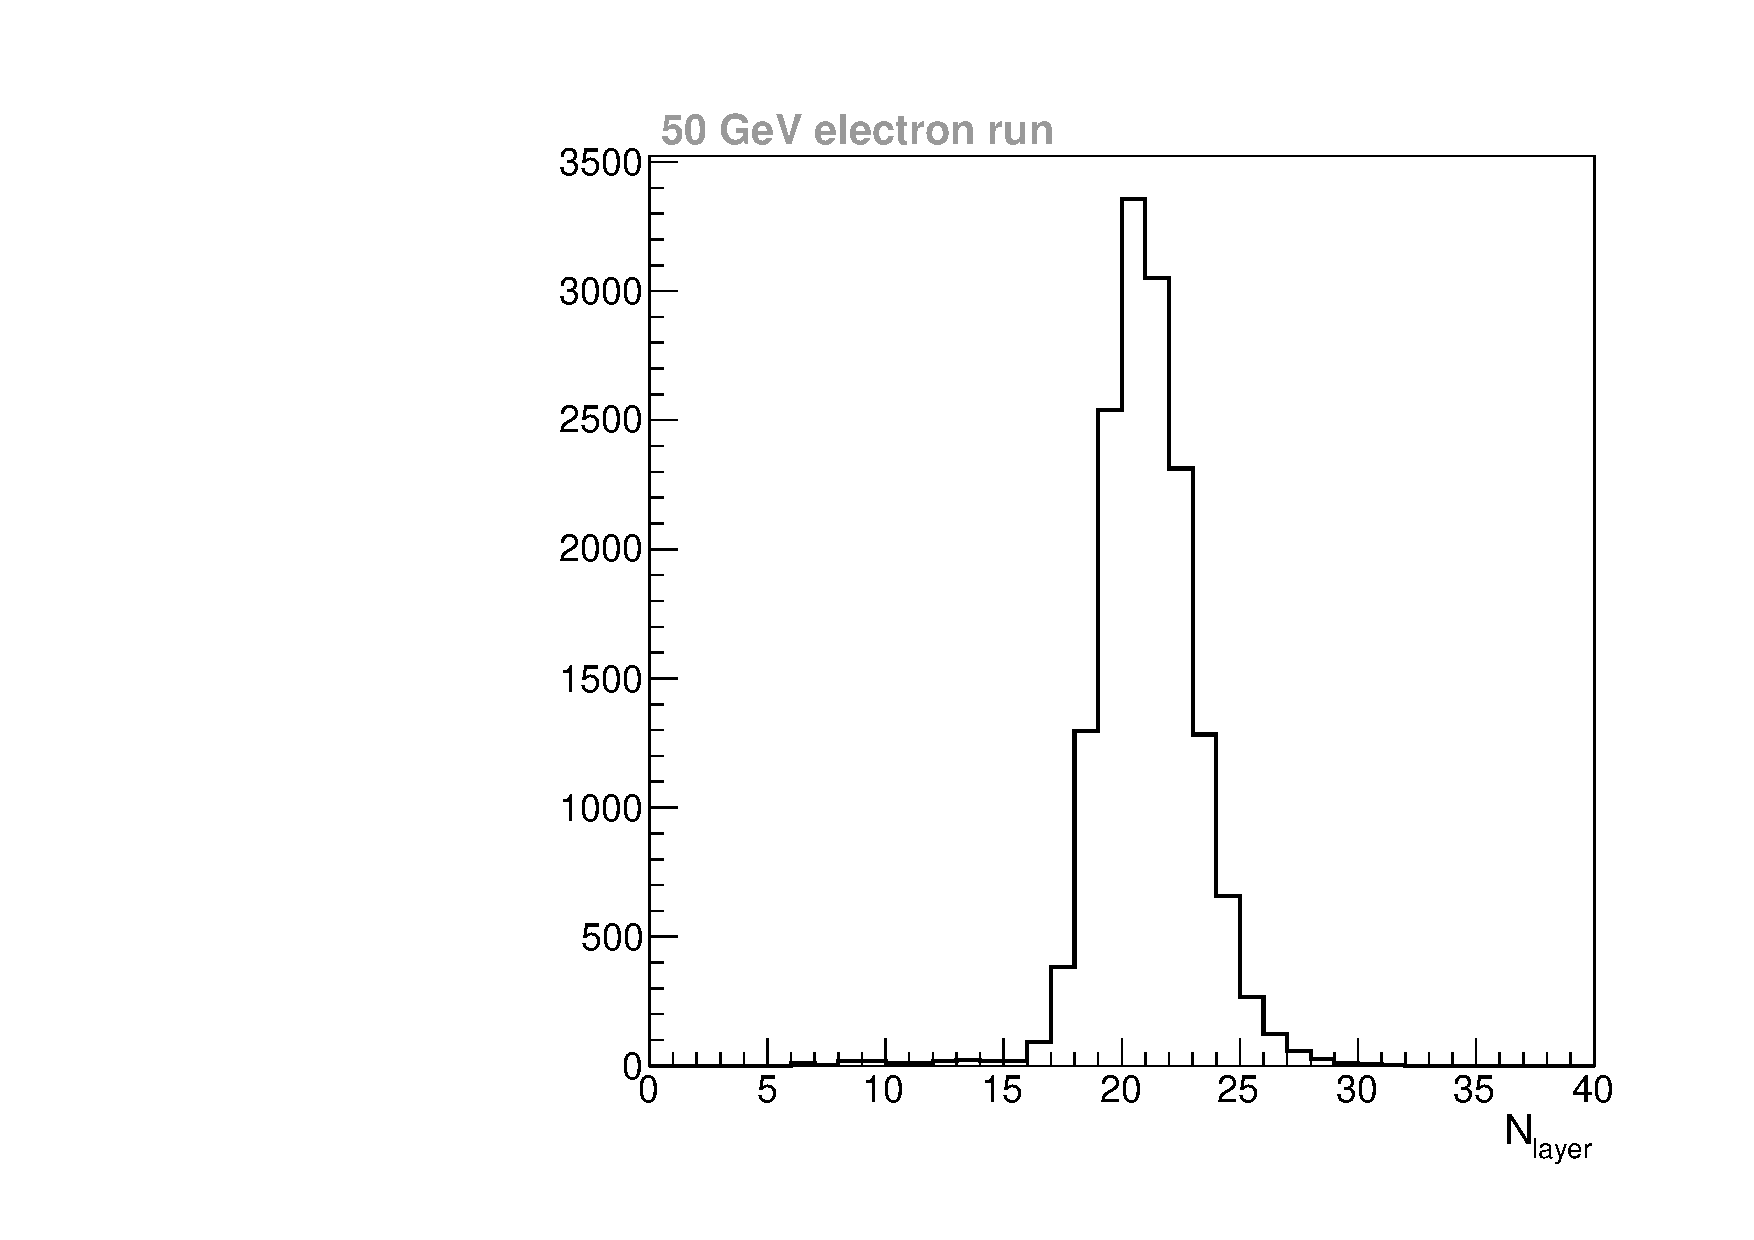
\includegraphics[width=.5\textwidth]{Digitizer/figs/Nlayer_e-_50GeV.pdf}}
%    \subfigure[]{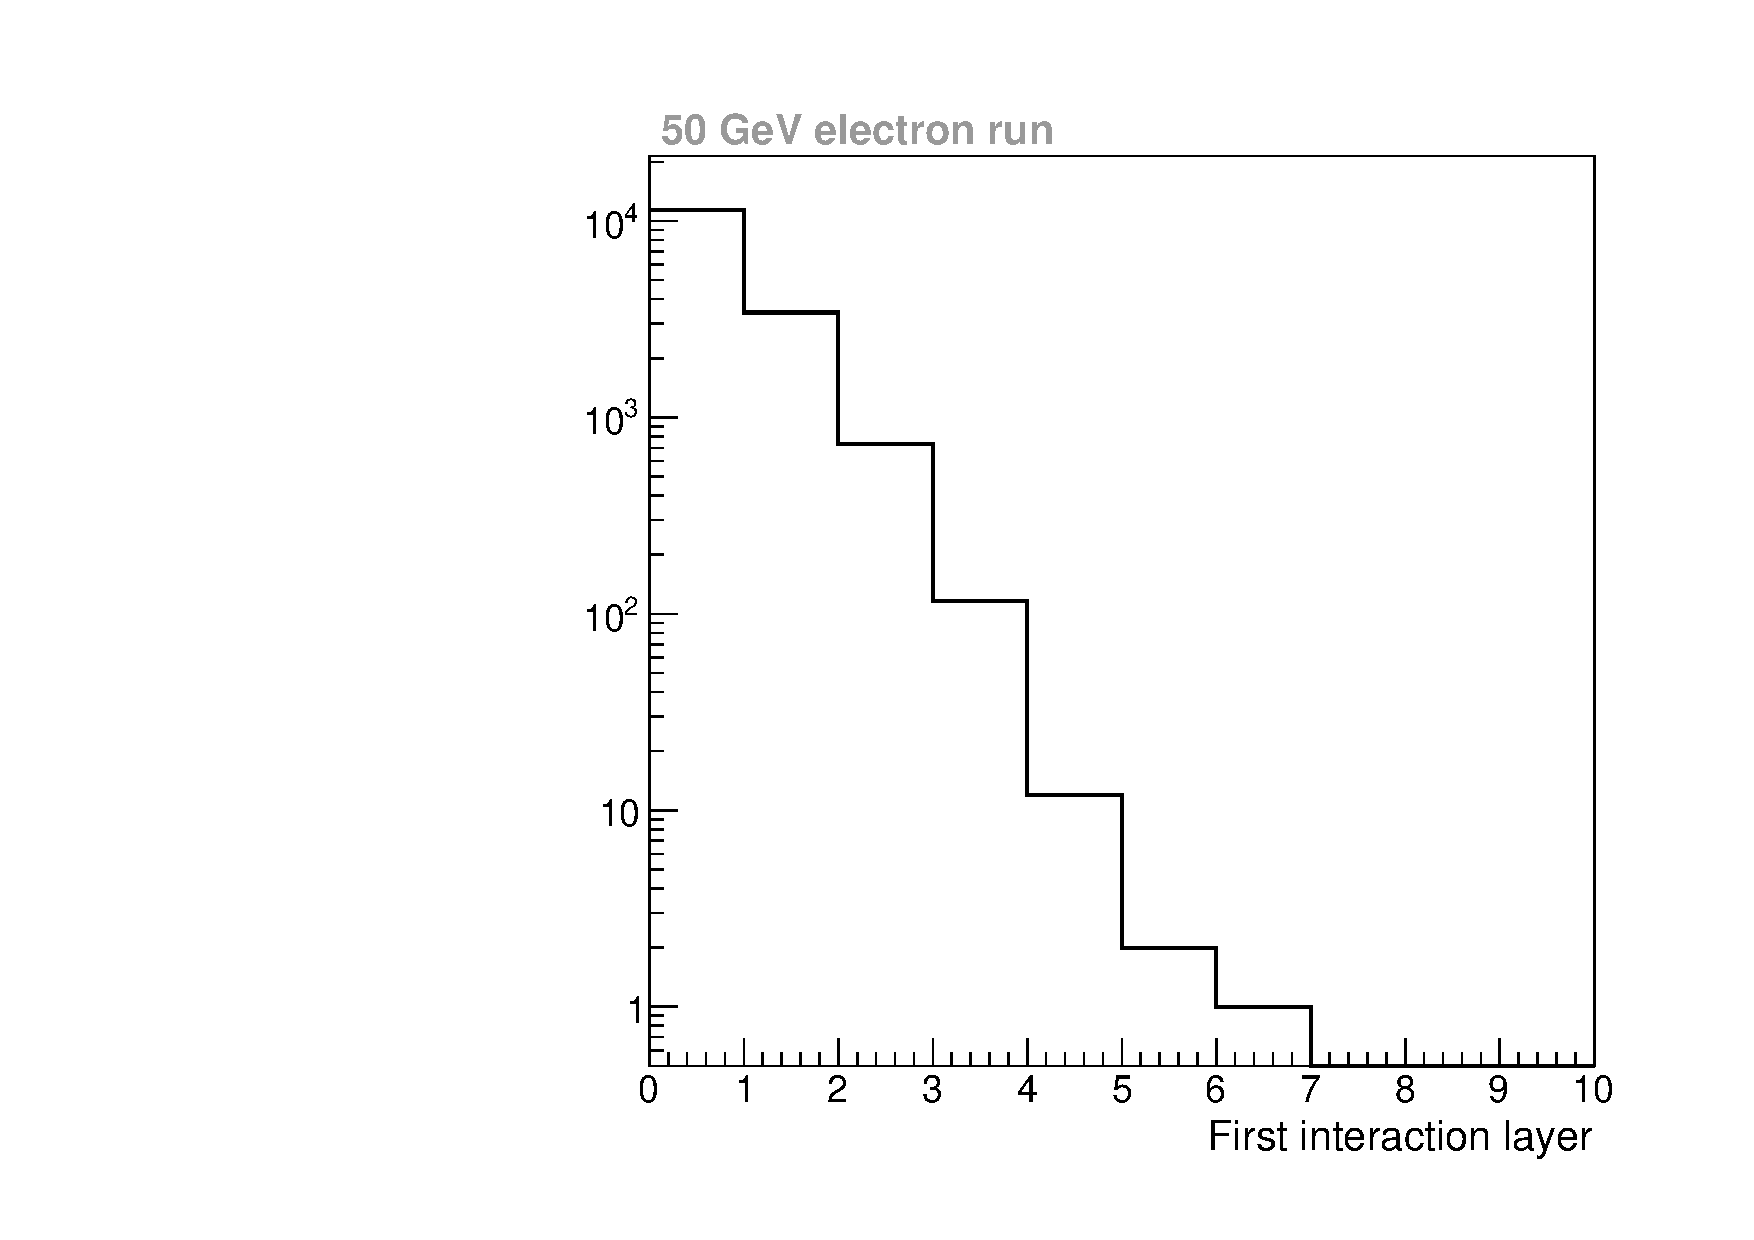
\includegraphics[width=.5\textwidth]{Digitizer/figs/Begin_e-_50GeV.pdf}}
%    \caption{(a): Distribution du nombre plans avec au moins un coup pour un échantillon de données de gerbes électromagnétiques à 50 GeV (la coupure sur le nombre de plan n'a pas été appliquée sur cette figure). (b): Distribution du premier plan d’interaction pour un échantillon de données de gerbes électromagnétiques à 50 GeV (la coupure sur le premier plan d'interaction n'a pas été appliquée sur cette figure)\label{fig.e-_begin_layer}}
%  \end{figure}
\end{enumerate}
Ces trois conditions utilisent principalement le fait que les gerbes électromagnétiques sont très compactes, en comparaison aux gerbes hadroniques. En effet, la longueur de radiation $X_0$ est de 1.75 $cm$ dans le fer, tandis que la longueur d'interaction est de 20.4 $cm$ pour les pions (16.8 $cm$ pour les protons).
La figure~\ref{fig:electron_control} dans le chapitre~\ref{chap.sdhcal} montre les distributions de chacune de ces variables pour un échantillon de simulation de gerbes électromagnétiques à 50 $GeV$. 
\begin{table}[!ht]
  \begin{center}
    \begin{tabular}{c|c|c}
      \rowcolor{black!20!white}Energie & Efficacité (EM) & Efficacité (HAD) \\
      \rowcolor{black!5!white}\hline
      \rowcolor{black!5!white}$10~GeV$ & $99.1\pm 0.07\%$ & $8.2\pm 0.19\%$ \\
      \rowcolor{black!5!white}$20~GeV$ & $99.1\pm 0.07\%$ & $4.4\pm 0.15\%$\\
      \rowcolor{black!5!white}$30~GeV$ & $98.8\pm 0.08\%$ & $2.2\pm 0.10\%$\\
      \rowcolor{black!5!white}$40~GeV$ & $98.5\pm 0.09\%$ & $1.2\pm 0.08\%$\\
      \rowcolor{black!5!white}$50~GeV$ & $97.9\pm 0.10\%$ & $0.8\pm 0.06\%$\\
    \end{tabular}
  \end{center}  
  \caption{Efficacité de sélection des gerbes électromagnétiques ($2^{ème}$ colonne) en fonction de l'énergie de la particule incidente, et efficacité de sélection des gerbes hadroniques, calculée avec les critères de sélection des gerbes électromagnétiques. Ces efficacités sont déterminées avec des échantillons de simulation.}
  \label{tab.e_sel_eff}
\end{table}
\begin{figure}[!ht]
  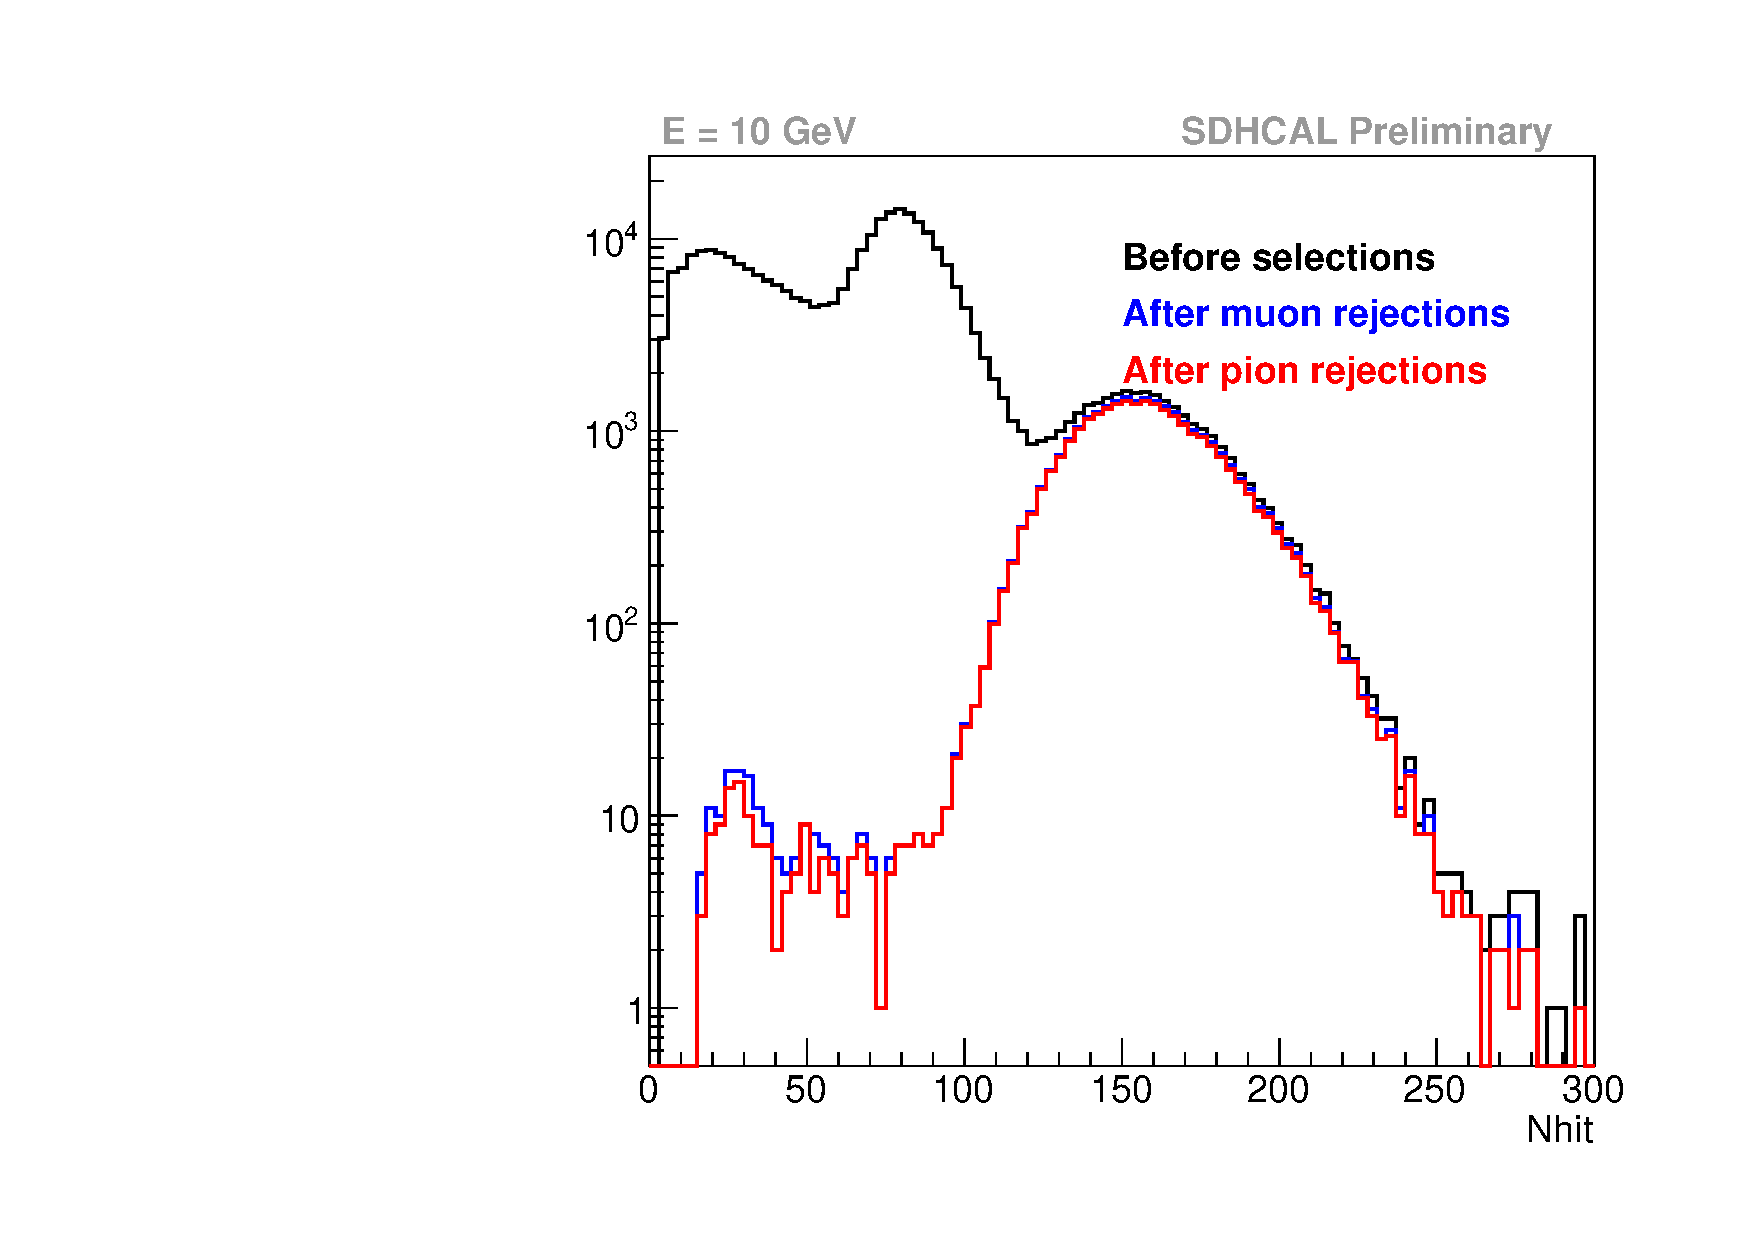
\includegraphics[width=.45\textwidth]{Digitizer/figs/selection715725.pdf}
  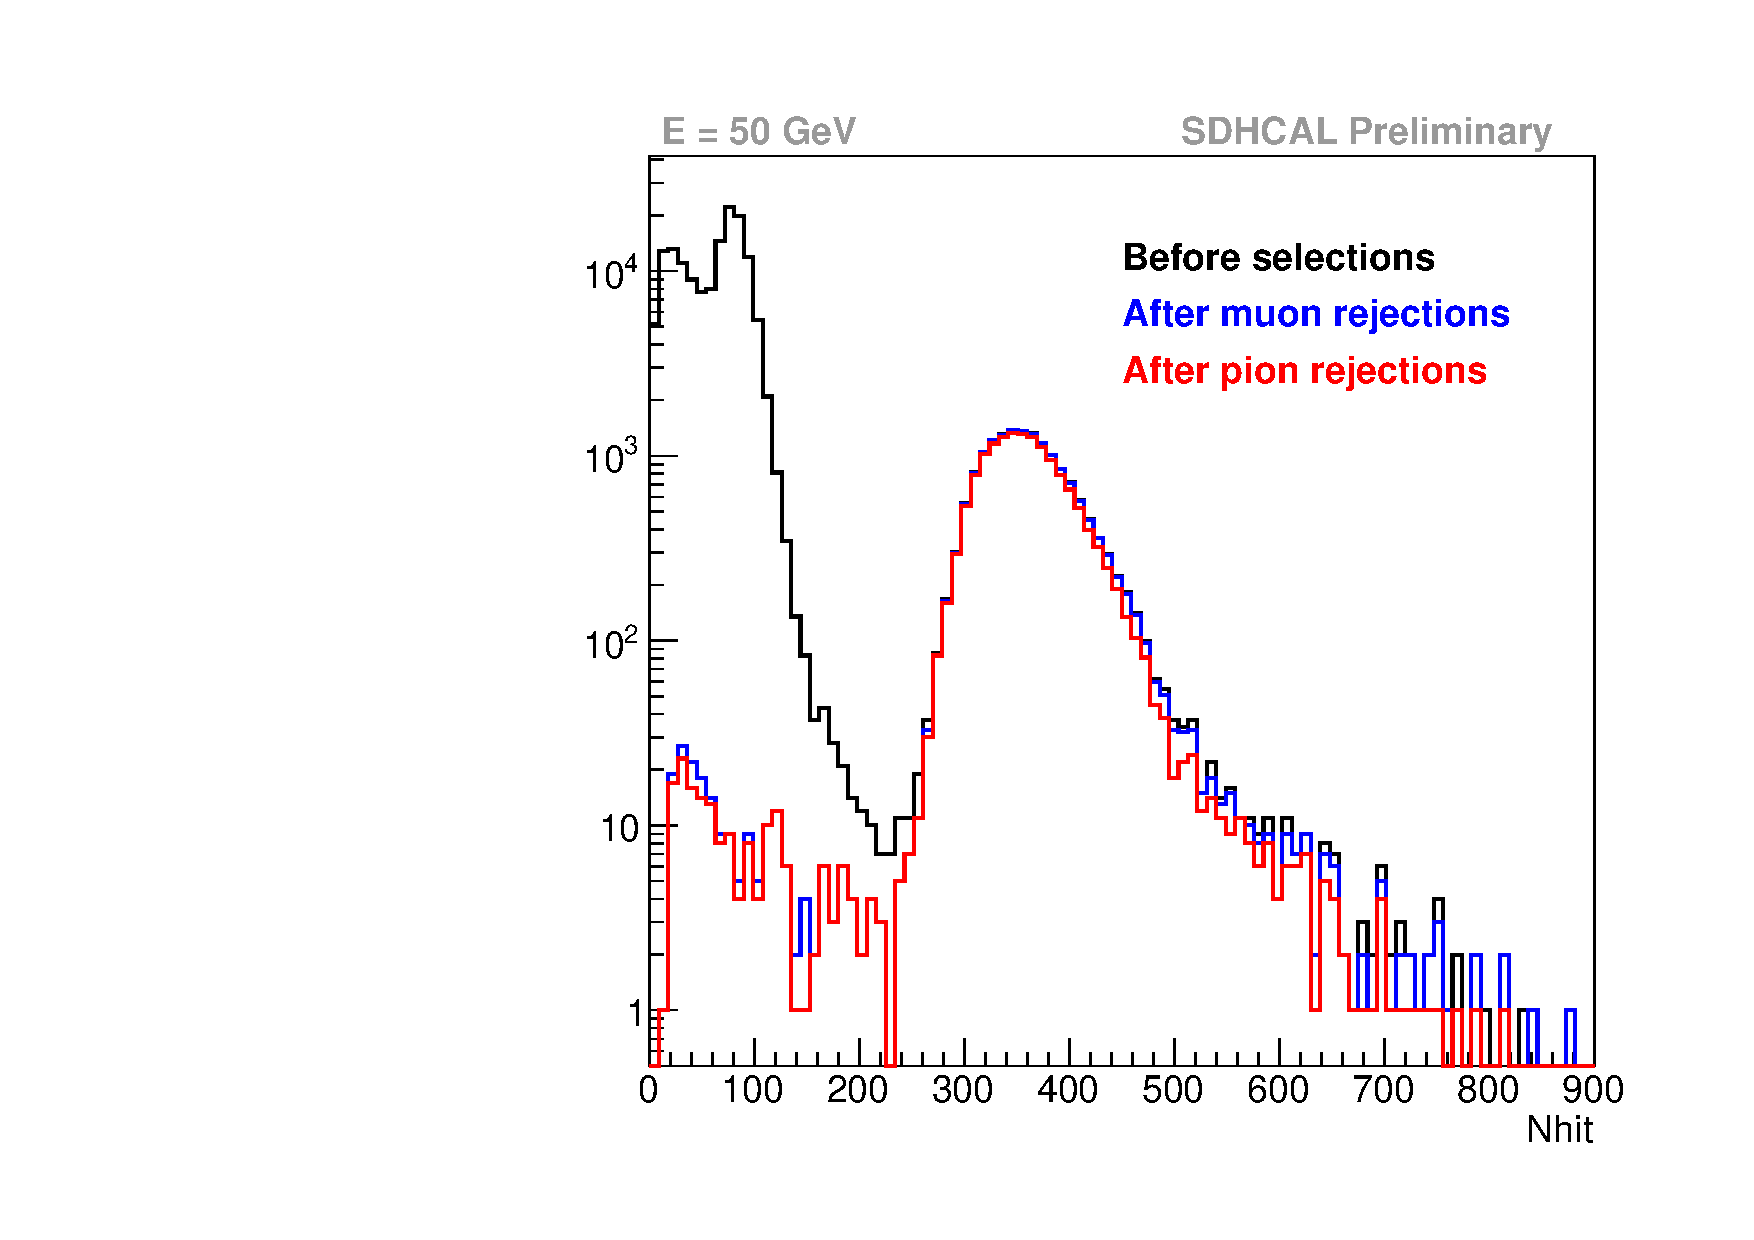
\includegraphics[width=.45\textwidth]{Digitizer/figs/selection715716.pdf}
  \caption{Distribution du nombre de hits pour des échantillons de données d'électrons à 10 GeV (à gauche) et 50 GeV (à droite) avant l'application des critères de sélection (ligne noire), après les coupures muons (ligne bleu) et après les coupures pour rejeter les gerbes hadroniques (ligne rouge). \label{fig.e-Selection}}
\end{figure}
Le tableau~\ref{tab.e_sel_eff} présente l'efficacité de sélection des gerbes électromagnétiques en fonction de l'énergie. L'efficacité est mesurée avec la simulation et correspond au rapport entre le nombre d'événements simulés et le nombre d'événements identifiés comme gerbes électromagnétiques. Les mêmes critères de sélection sont appliqués à des échantillons de simulation de gerbes hadroniques. Les efficacités ainsi estimées sont aussi montrées dans le tableau~\ref{tab.e_sel_eff}. Ces différents critères permettent ainsi une très bonne identification des gerbes électromagnétiques avec plus de 98$\%$ d'efficacité de sélection sur toute la gamme. Le taux de gerbes hadroniques conservées après l'application de ces critères est faible au dessus de 30 $GeV$. A plus basse énergie, la fraction électromagnétique des gerbes hadroniques identifiées comme gerbes électromagnétiques a été étudiée. Elle est approximée en mesurant le rapport de l'énergie déposée par des électrons, des positons ou des photons sur l'énergie totale déposée dans le calorimètre. La valeur moyenne de cette fraction électromagnétique pour les gerbes hadroniques identifiées comme gerbes électromagnétiques est proche de 80$\%$ à 10 $GeV$. Nous avons aussi vérifié que le nombre moyen de hits pour les gerbes hadroniques identifiées comme cascades électromagnétiques, est proche de celui des gerbes électromagnétiques. A 10 $GeV$, la moyenne de nombre du hits dans les gerbes hadroniques mal identifiées est environ 172 alors qu'il y a en moyenne 168 hits dans les gerbes électromagnétiques. 
La figure~\ref{fig.e-Selection} montre les distributions de nombre de hits pour des échantillons de données d'électrons à 10 GeV et 50 GeV avant les coupures, après les coupures muons et enfin après les coupures pions.
\begin{figure}[!ht]
    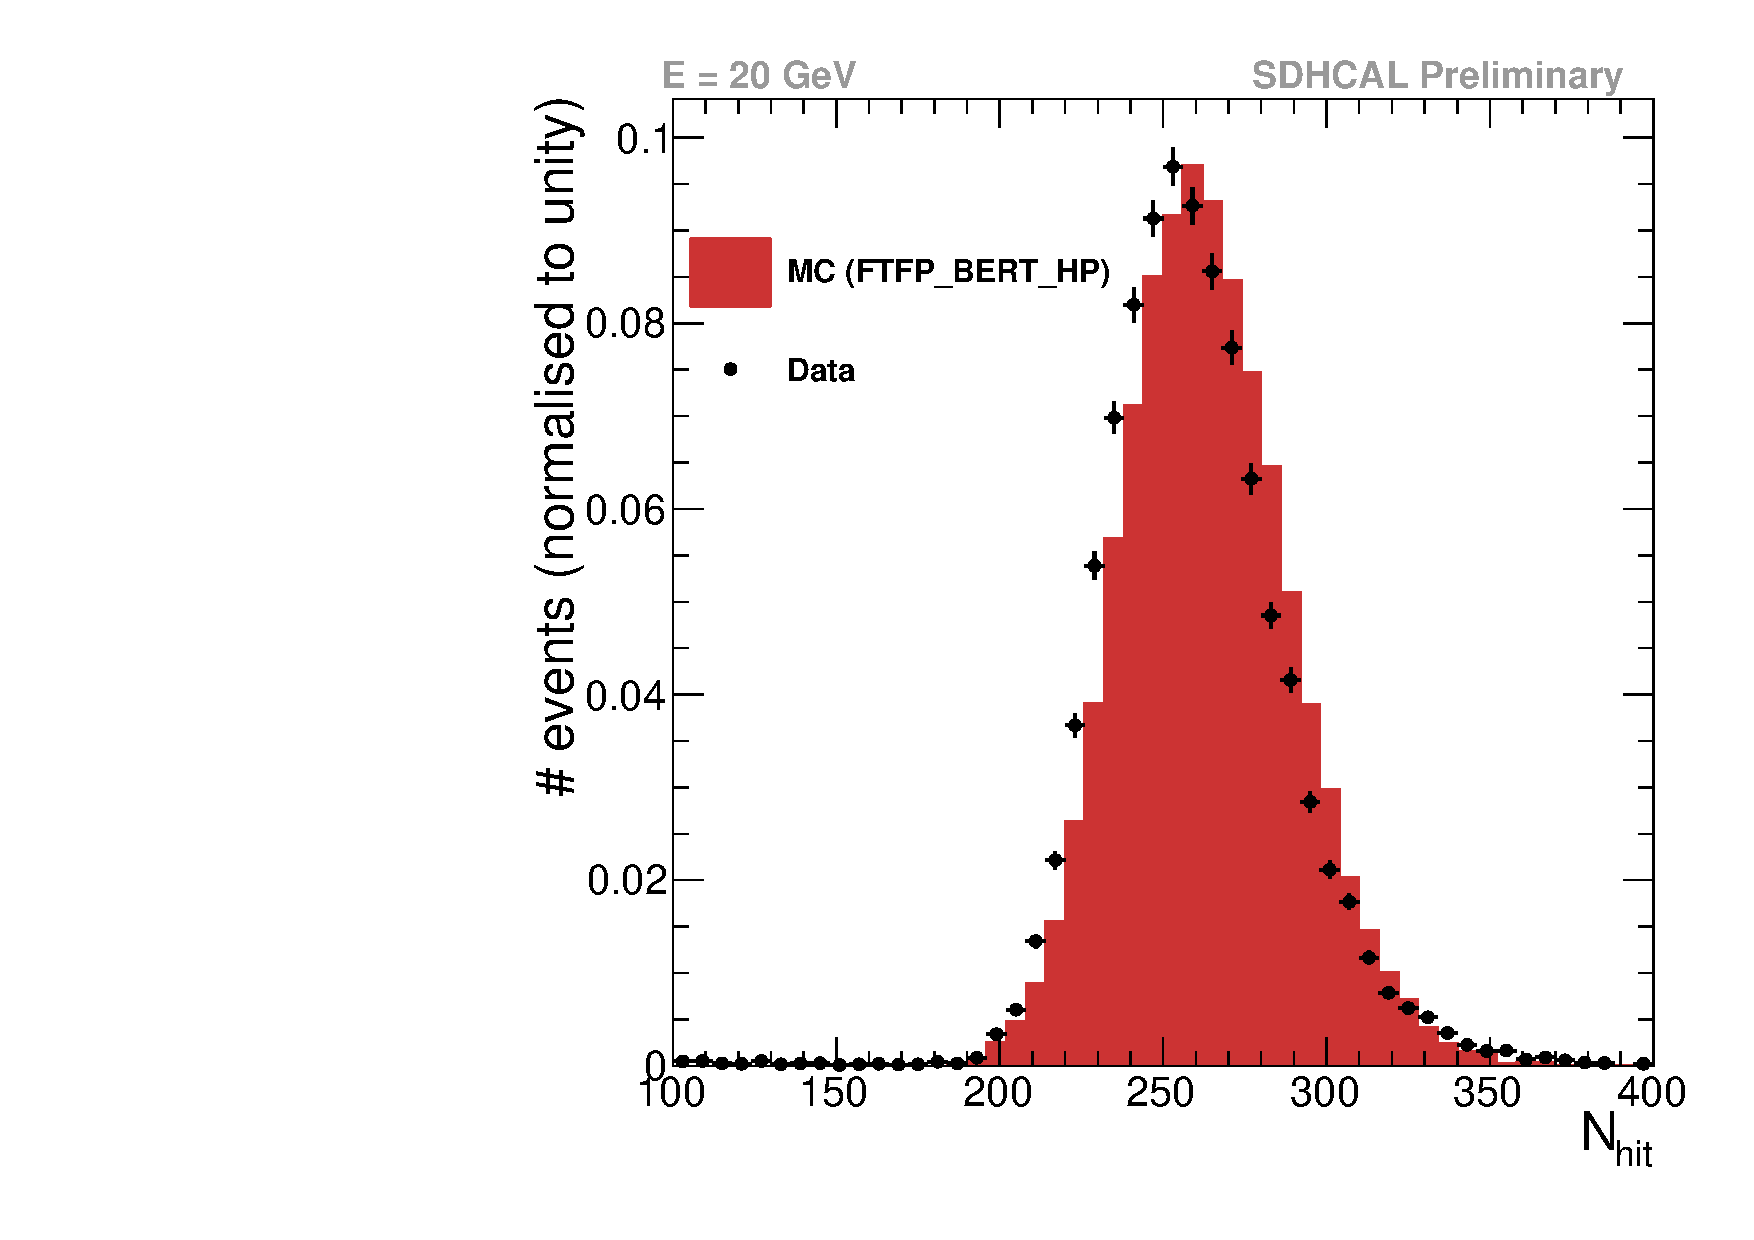
\includegraphics[width=.45\textwidth]{Digitizer/figs/nhit_e-_20GeV_AugSep2012.pdf}
    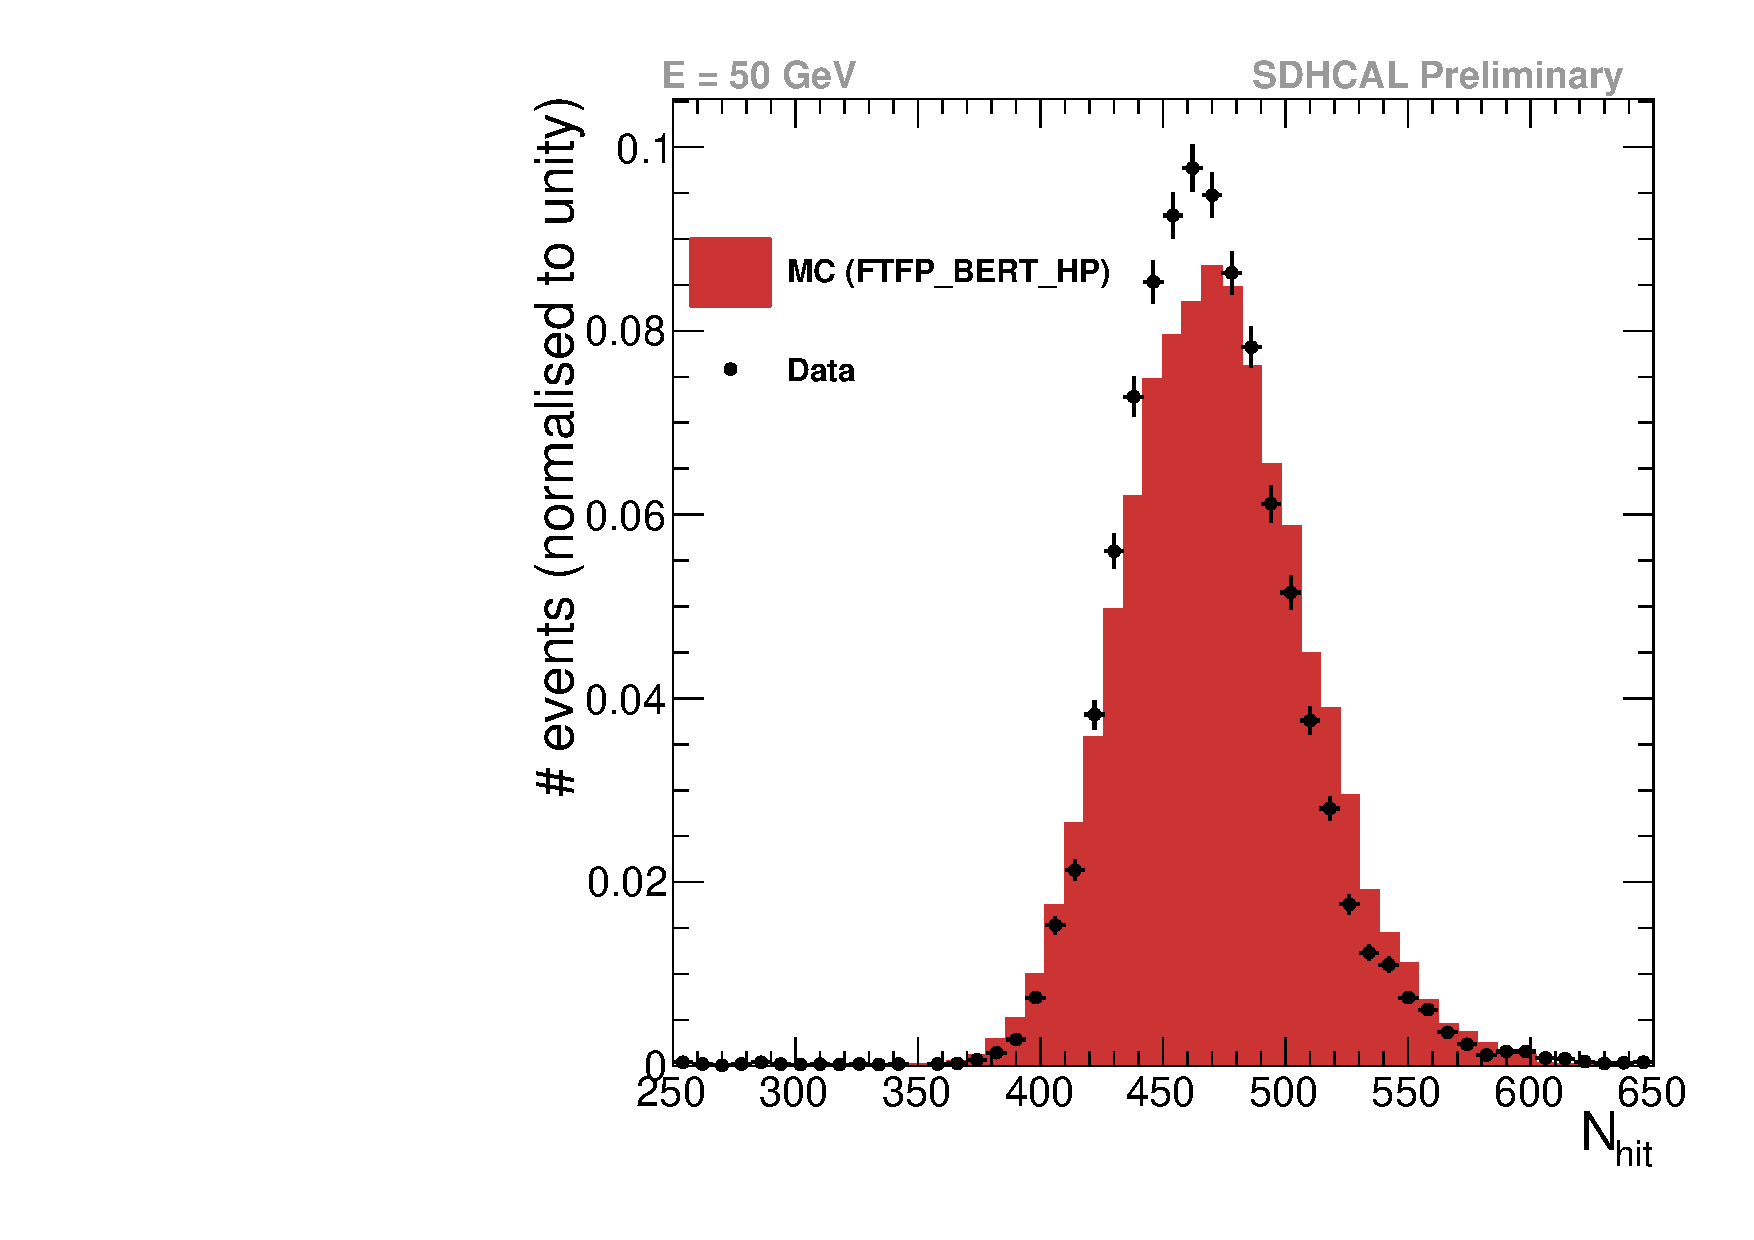
\includegraphics[width=.45\textwidth]{Digitizer/figs/nhit_e-_50GeV_AugSep2012.pdf}
    \caption{Distribution de nombre de hits pour des échantillons d'électrons de 20 GeV (à gauche) et 50 GeV (à droite). Les données sont représentées par des cercles noirs et la simulation par les histogrammes rouges.}
  \label{fig.nhite-_dist}
\end{figure}
\begin{figure}[!ht]
  \centering
  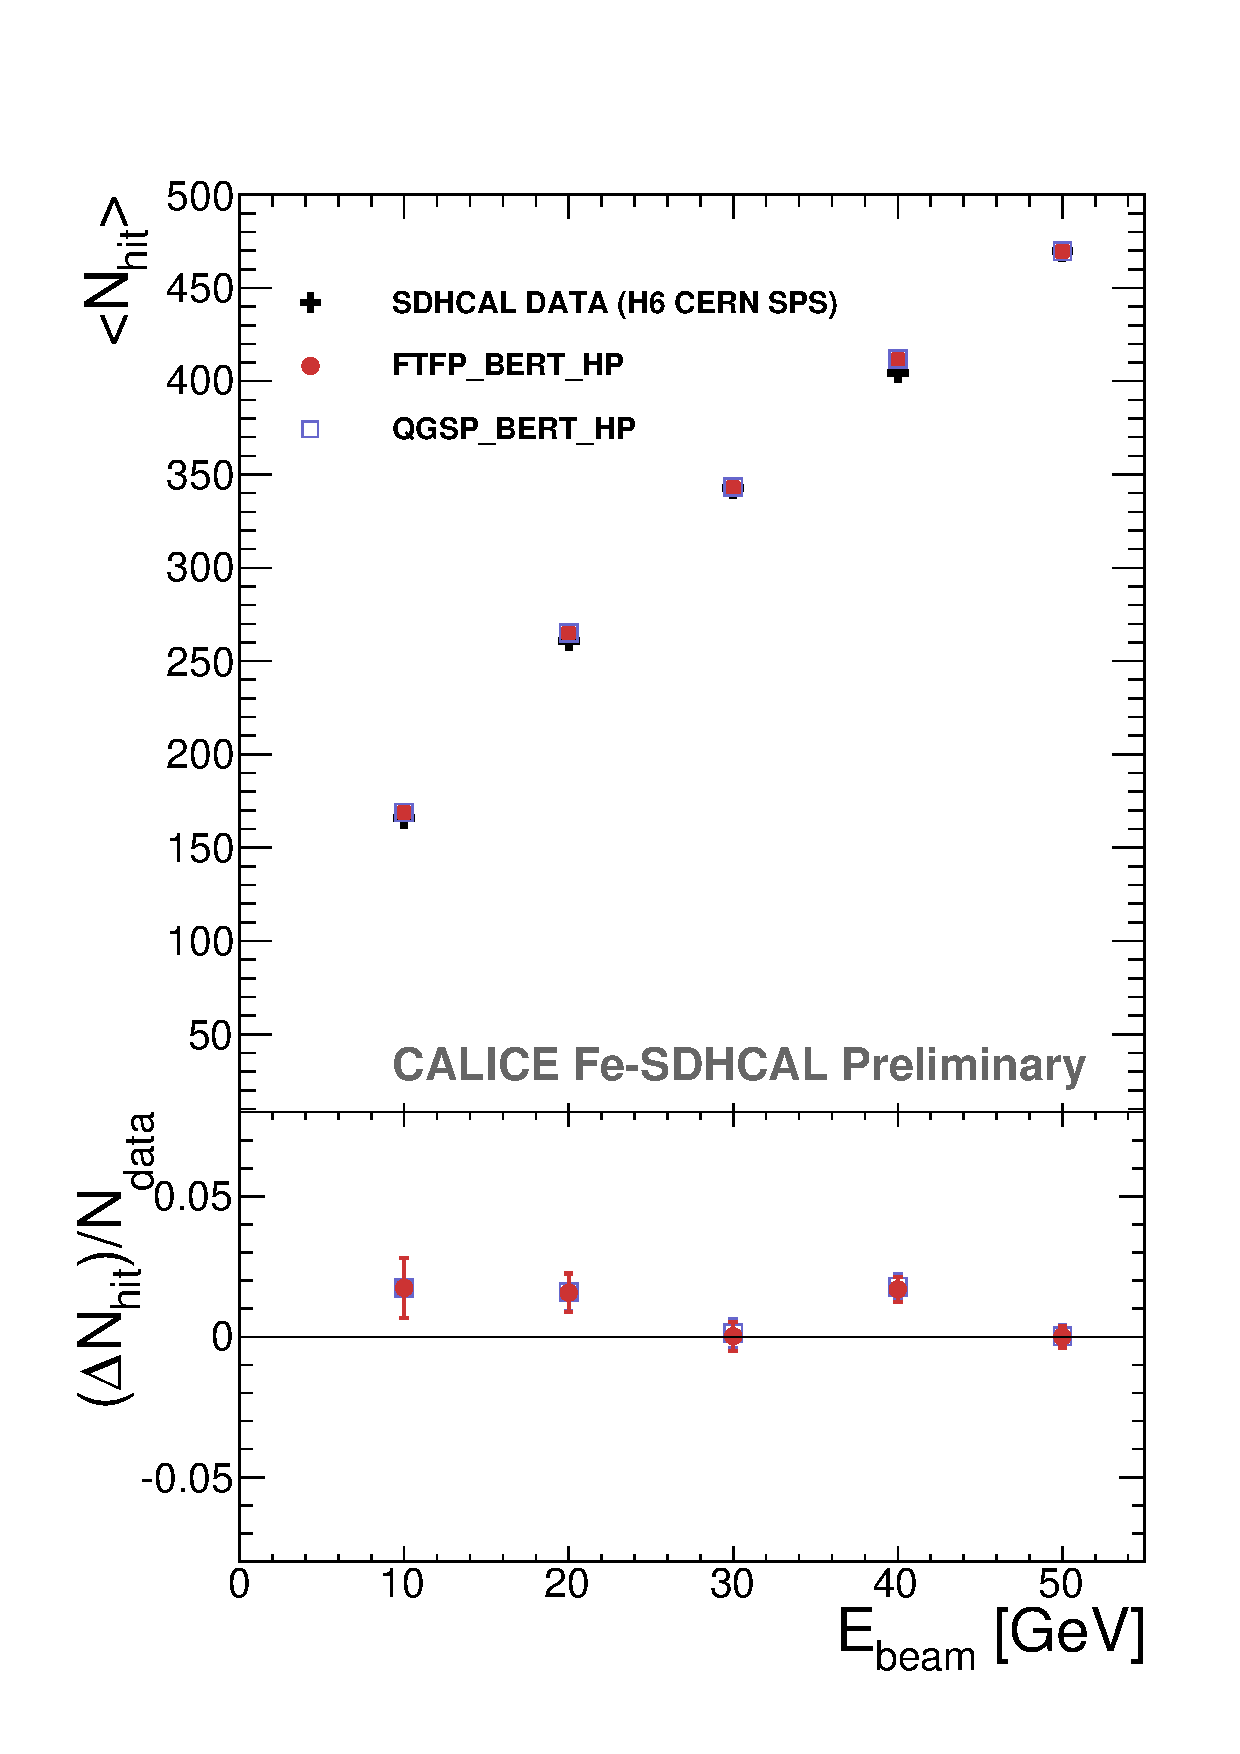
\includegraphics[width=0.5\textwidth]{Digitizer/figs/NHITELECTRON.pdf}
  \caption{Moyenne du nombre de hits pour des échantillons d'électrons en fonction de l’énergie du faisceau. Les données sont représentées par des croix noires, et la simulation par des cercles rouges (FTFP\_BERT\_HP) et des carrés bleus (QGSP\_BERT\_HP). La déviation relative est aussi présentée.}
  \label{fig.nhite-}
\end{figure}

La figure~\ref{fig.nhite-_dist} présente les distributions de nombre de hits pour des échantillons de gerbes électromagnétiques à 20 et 50 $GeV$ pour les données et la simulation. 
La figure~\ref{fig.nhite-} montre les valeurs moyennes du nombre de hits dans les gerbes électromagnétiques en fonction de l'énergie pour les données et la simulation. Les déviations relatives entre les données et la simulation définies comme $\frac{<N_{hit}^{sim}>-<N_{hit}^{data}>}{<N_{hit}^{data}>}$ sont aussi indiquées sur cette figure. Le nombre de cellules touchées par du bruit, estimé à 1.75 par événement physique (cf. section~\ref{sec.trivent} du chapitre~\ref{chap.sdhcal}), est ajoutée en quadrature aux incertitudes statistiques dans les données, puis reportée dans les barres d'erreur de la déviation relative. L'accord entre les données expérimentales et les deux listes physiques utilisées pour la simulation est très satisfaisant. Les déviations relatives sont inférieures à 3\% sur toute la gamme d'énergie. Ces résultats ont tendance à valider l'algorithme de modélisation et son paramétrage. 

%%%%%%%%%%%%%%%%%%%%%
\newpage
\subsubsection{Gerbes hadroniques}
La même procédure de sélection que celle décrite dans le chapitre~\ref{chap.sdhcal} est appliquée sur les données expérimentales et sur la simulation. 
\begin{figure}[!ht]
  \centering
  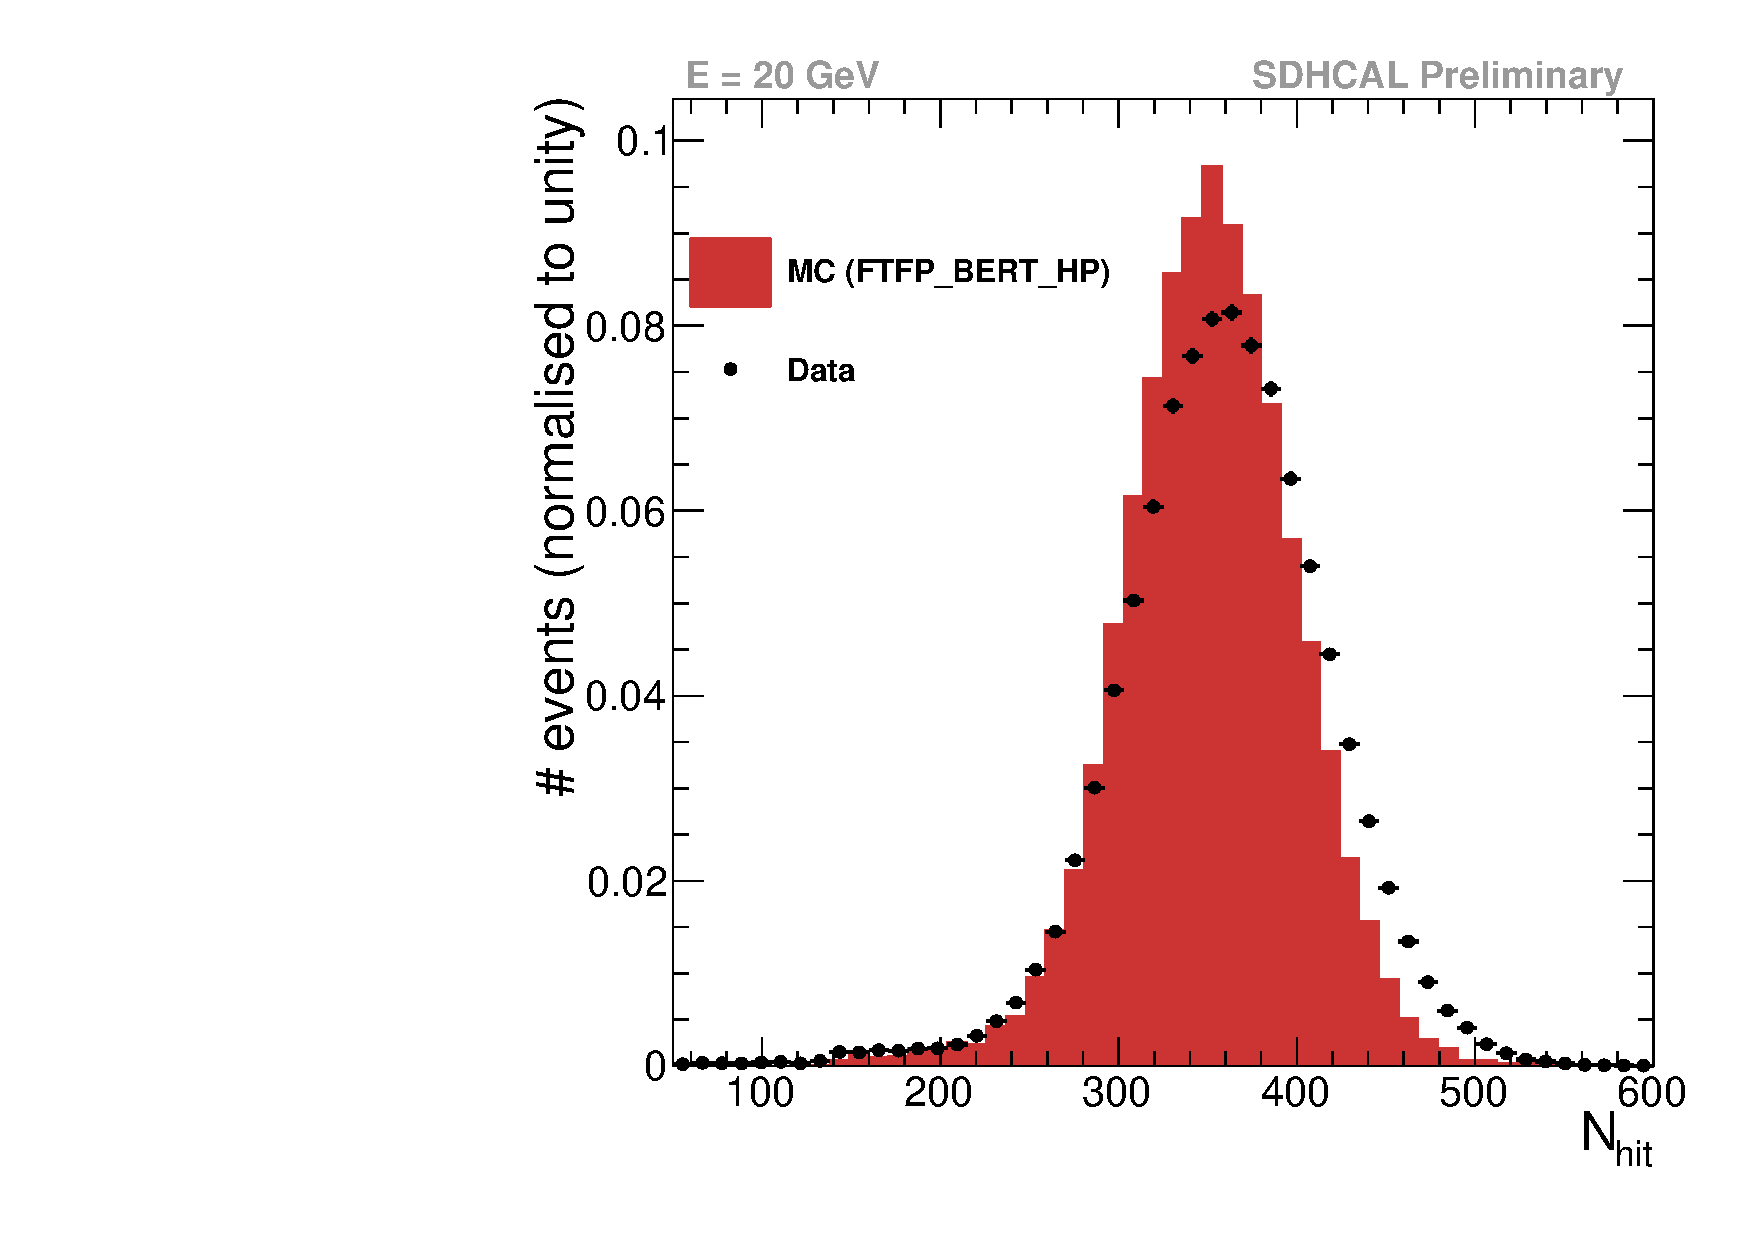
\includegraphics[width=.45\textwidth]{Digitizer/figs/nhit_pi-_20GeV_AugSep2012.pdf}
  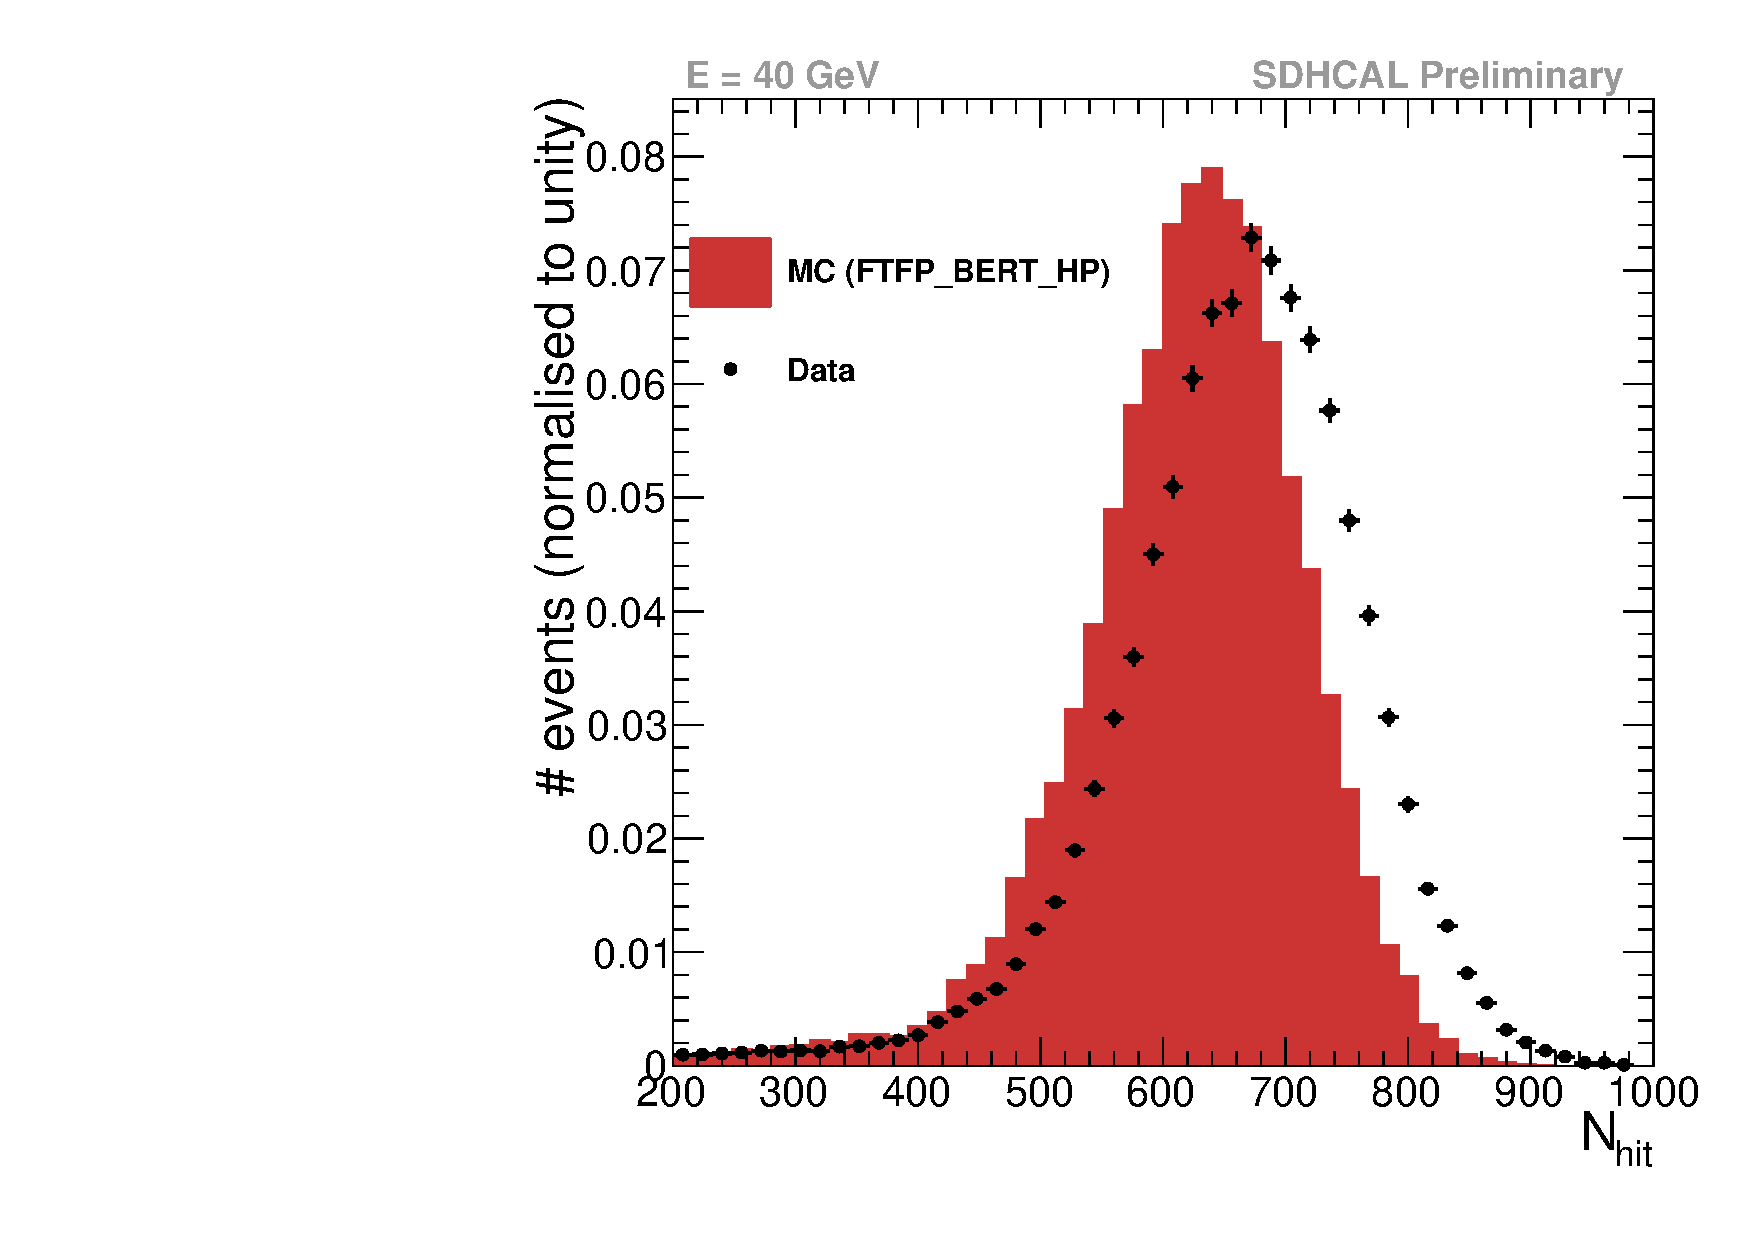
\includegraphics[width=.45\textwidth]{Digitizer/figs/nhit_pi-_40GeV_AugSep2012.pdf}
  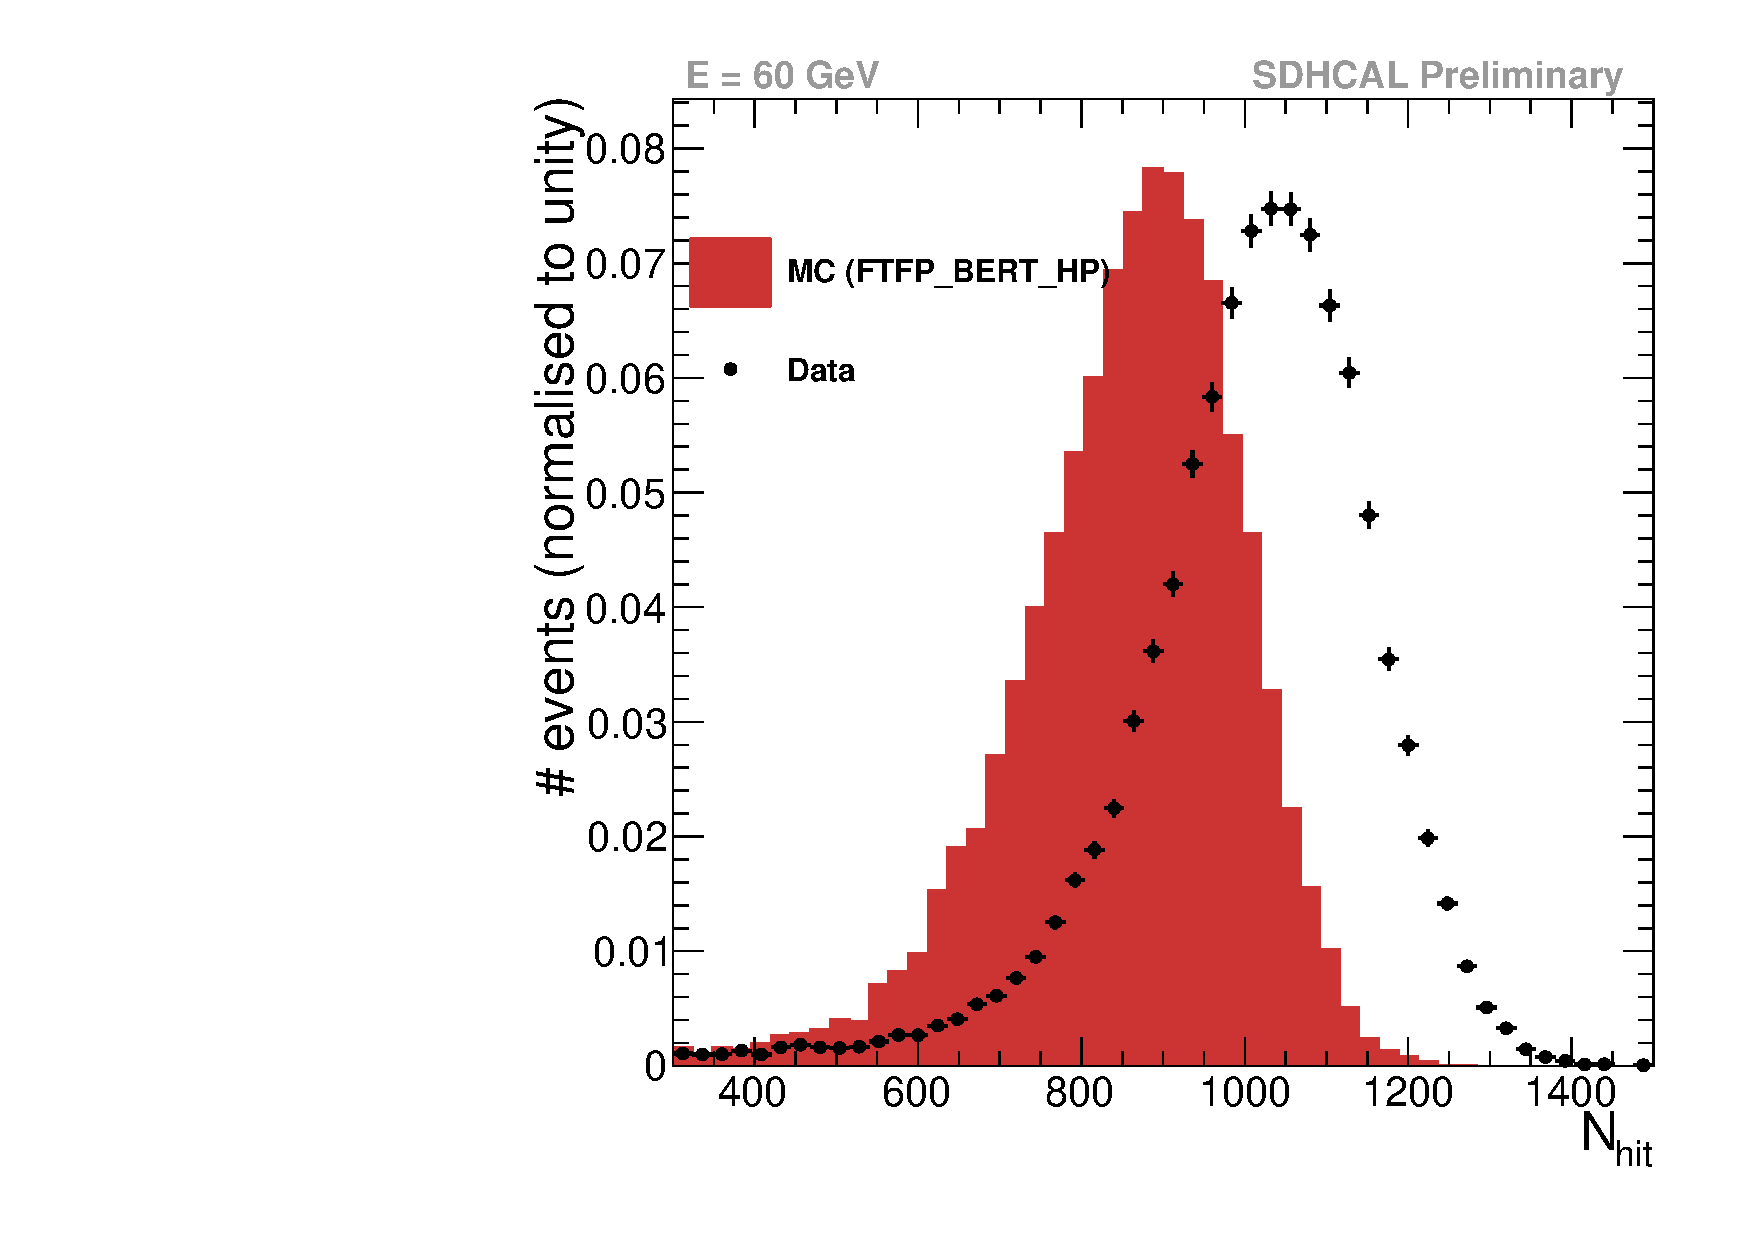
\includegraphics[width=.45\textwidth]{Digitizer/figs/nhit_pi-_60GeV_AugSep2012.pdf}
  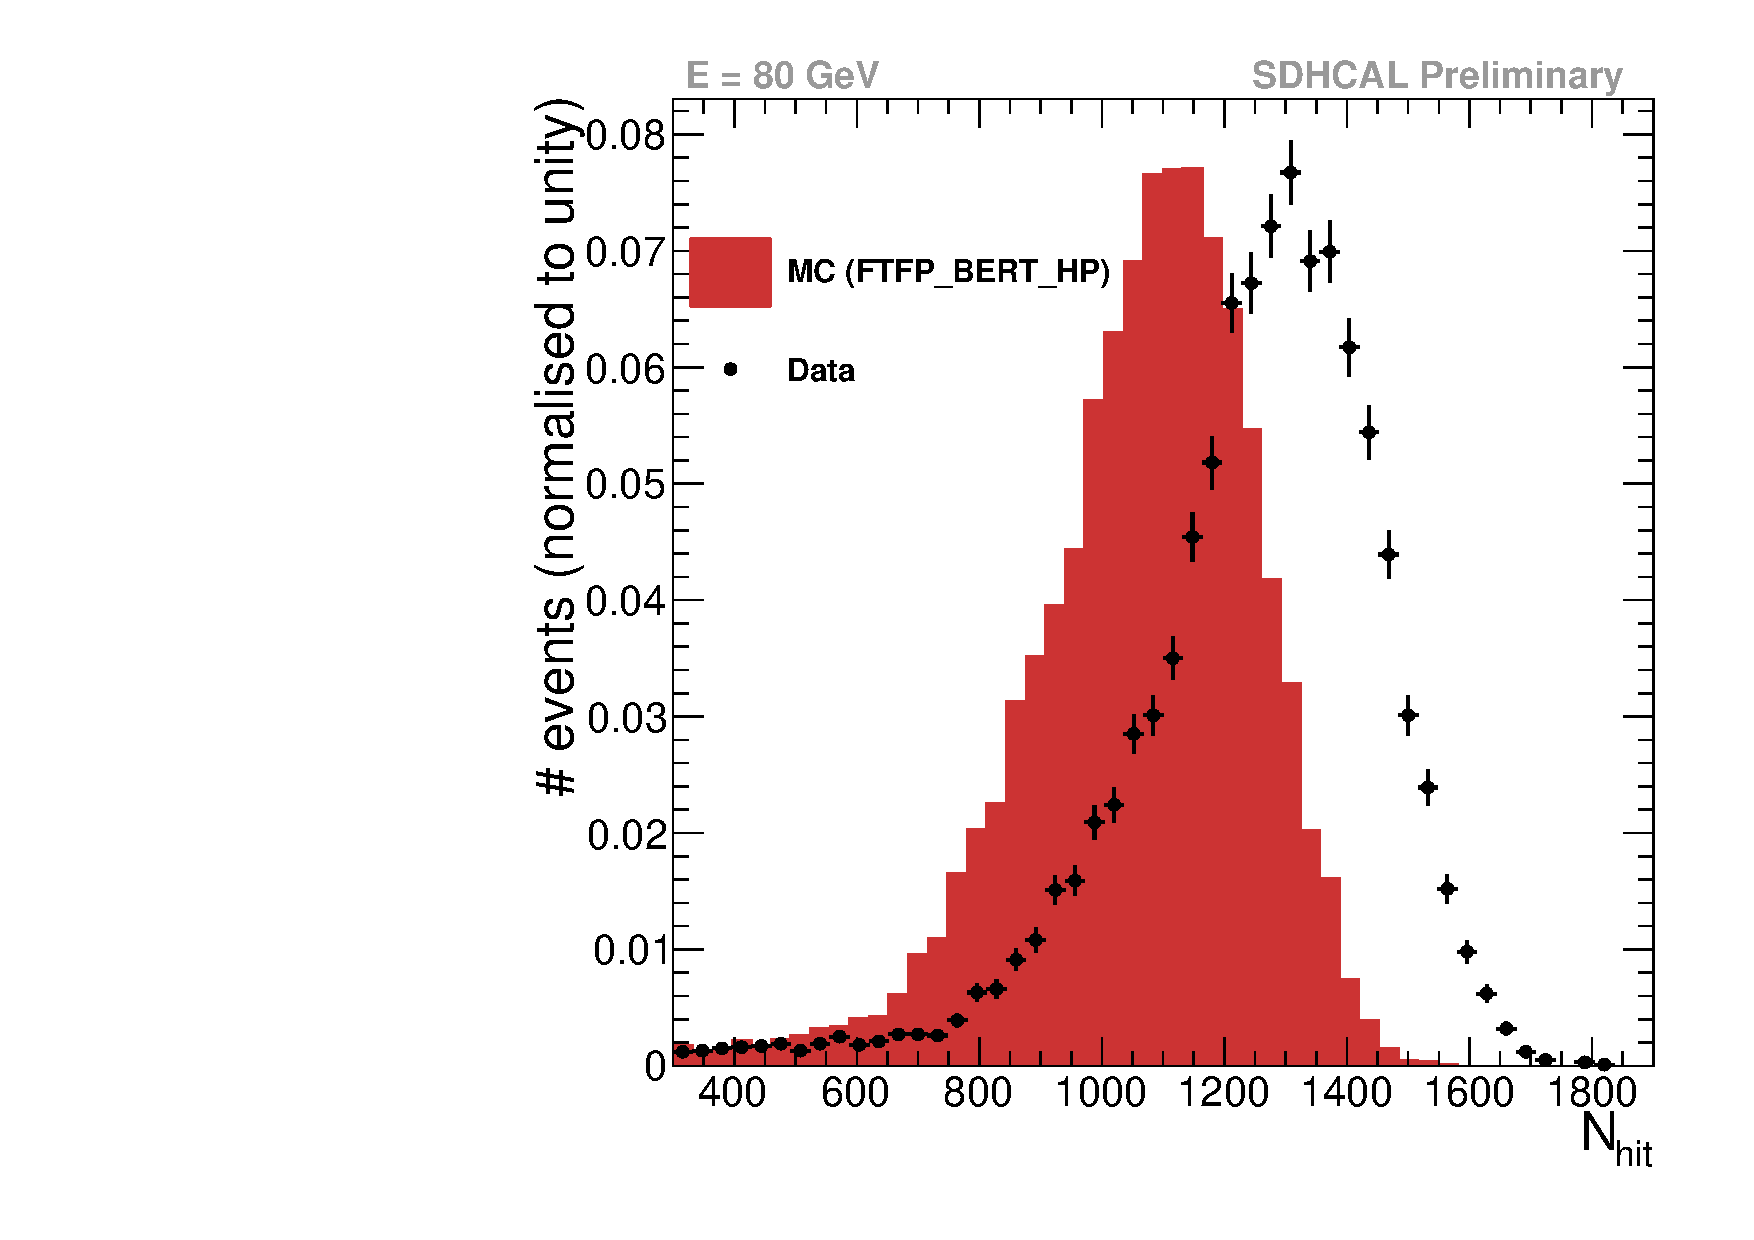
\includegraphics[width=.45\textwidth]{Digitizer/figs/nhit_pi-_80GeV_AugSep2012.pdf}
  \caption{Distribution du nombre de hits pour des échantillons de pions de 20 GeV (a), 40 GeV(b), 60 GeV (c) et 80 GeV (d). Les données sont représentées par des croix noires et la simulation (FTFP\_BERT\_HP) par les histogrammes rouges. \label{fig.pi-nhit}}
\end{figure}
La figure~\ref{fig.pi-nhit} montre les distributions du nombre total de hits pour des gerbes hadroniques à 20, 30, 60 et 80 $GeV$ pour les données et la simulation. Sur cette figure, la simulation est réalisée avec la liste physique FTFP\_BERT\_HP et les échantillons de données ont été enregistrés sur la ligne H6 du CERN. L'accord entre données et simulation semble raisonnable à basse énergie. A haute énergie, la simulation sous-estime le nombre total de hits des gerbes hadroniques.
\begin{figure}[!ht]
  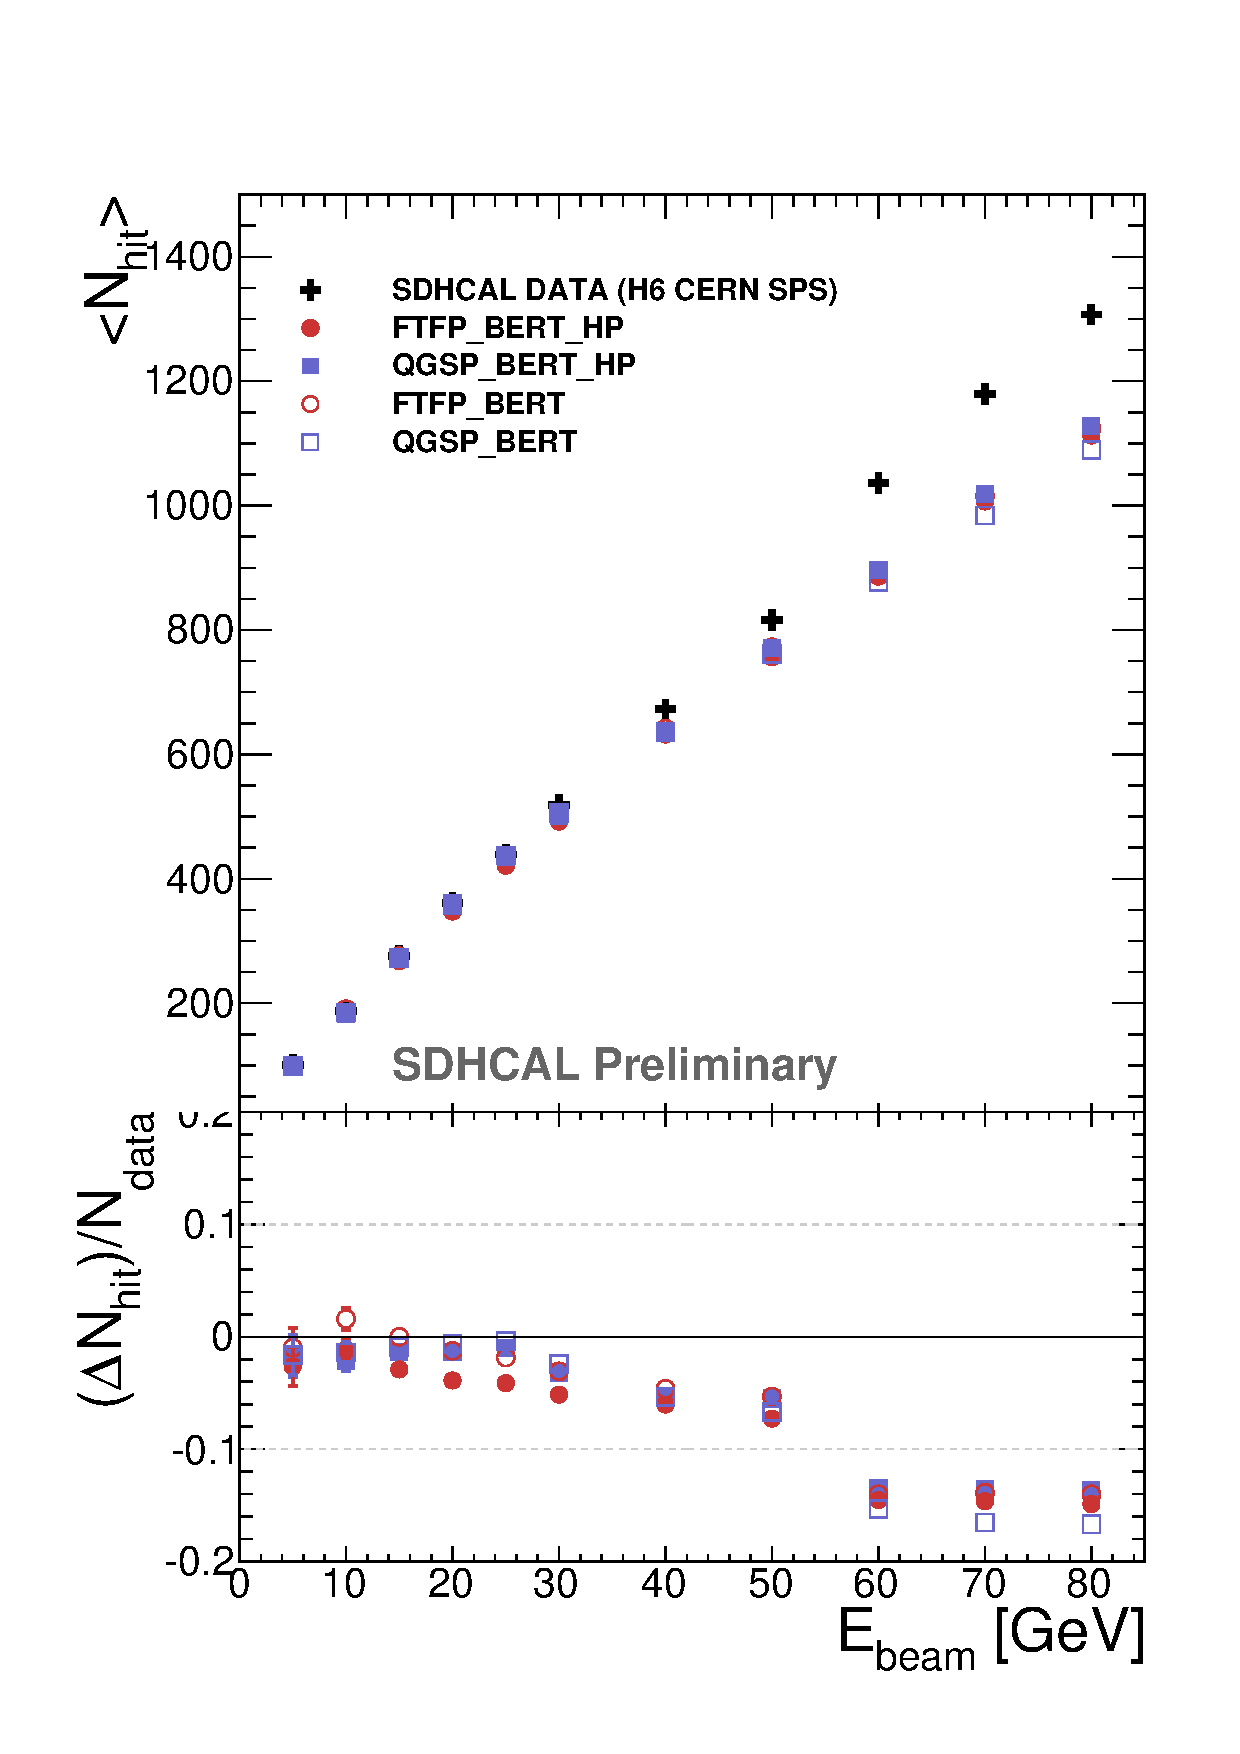
\includegraphics[width=.5\textwidth]{Digitizer/figs/NHITPIONHP.pdf}
  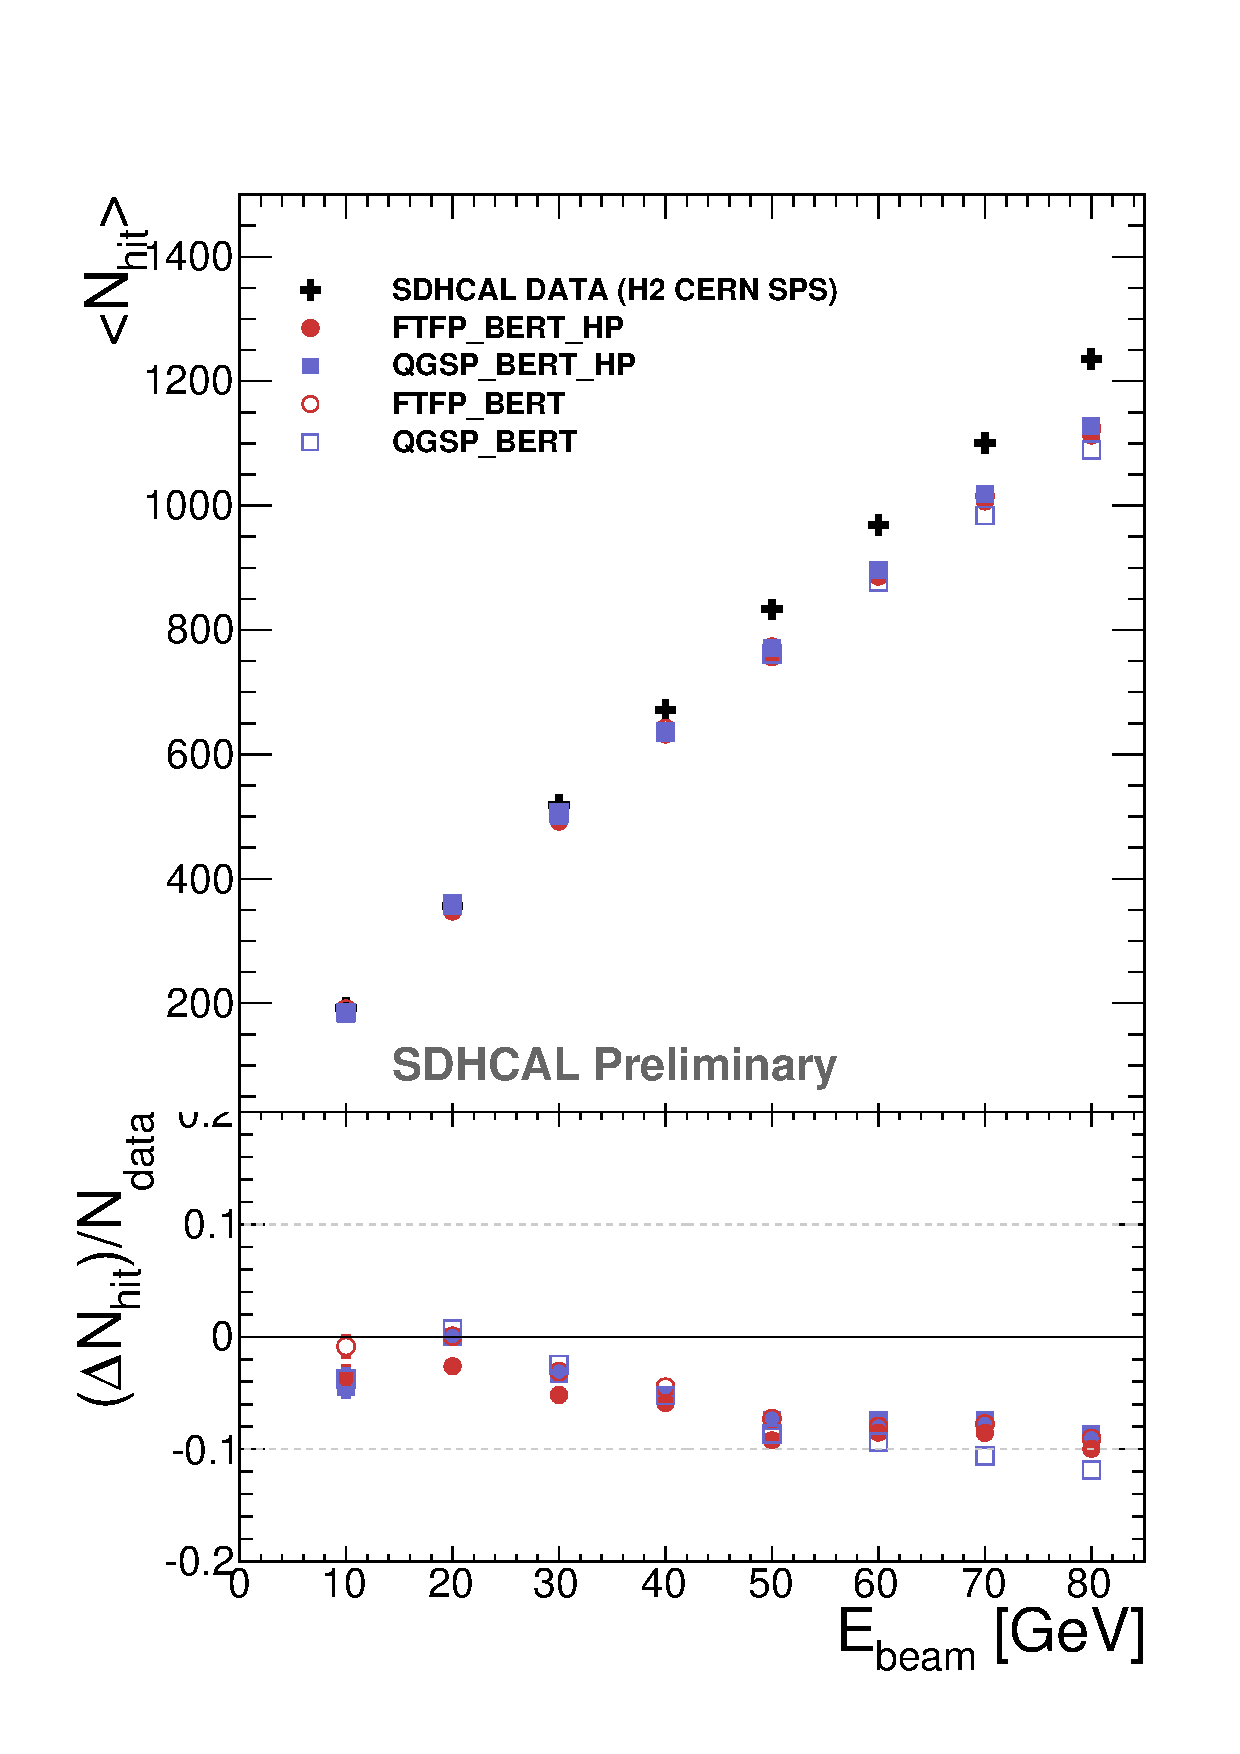
\includegraphics[width=.5\textwidth]{Digitizer/figs/NHITPION_NOV_HP.pdf}
  \caption{Nombre moyen de hits pour des gerbes hadroniques en fonction de l'énergie du faisceau pour des données (croix noires) enregistrées sur les lignes H6 (à gauche) et H2 (à droite) et les listes physiques FTFP\_BERT\_(HP) (cercles rouges) et QGSP\_BERT(\_HP) (carrés bleu). Les déviations relatives sont aussi présentées.}
  \label{fig.nhit_pi-_ebeam}
\end{figure}
Ces différences sont confirmées par la figure~\ref{fig.nhit_pi-_ebeam} qui montre le nombre total moyen de hits dans les gerbes hadroniques en fonction de l'énergie du faisceau pour les données et plusieurs listes physiques de simulation. La figure de gauche est réalisée avec des données enregistrées sur la ligne H6 du CERN et la figure de droite avec des données de la ligne H2. Rappelons qu'à la différence de la ligne H2, la ligne H6 est contaminée par des protons, avec jusqu'à environ 60 $\%$ de proton à 100 $GeV$. La déviation relative définie comme $\frac{<N_{hit}^{sim}>-<N_{hit}^{data}>}{<N_{hit}^{data}>}$ est aussi montrée sur ces figures. Comme pour les gerbes électromgnétiques, le nombre de cellules touchées par du bruit est pris en compte dans les barres d'erreur. Un bon accord entre la simulation et les données est trouvé jusqu'à 30 $GeV$. A partir de 40 $GeV$, l'accord se dégrade. La déviation relative entre les données et les différentes listes physiques est d'environ 15$\%$ à partir de 60$GeV$ pour les données de la ligne H6 et environ 10$\%$ pour la ligne H2. Ces figures montrent aussi que l'option de haute précision pour les neutrons n'a qu'une faible influence sur le nombre total de hits des gerbes hadroniques. Ces faibles différences s'expliquent par la faible sensibilité du SDHCAL aux neutrons. 
\begin{figure}[!ht]
  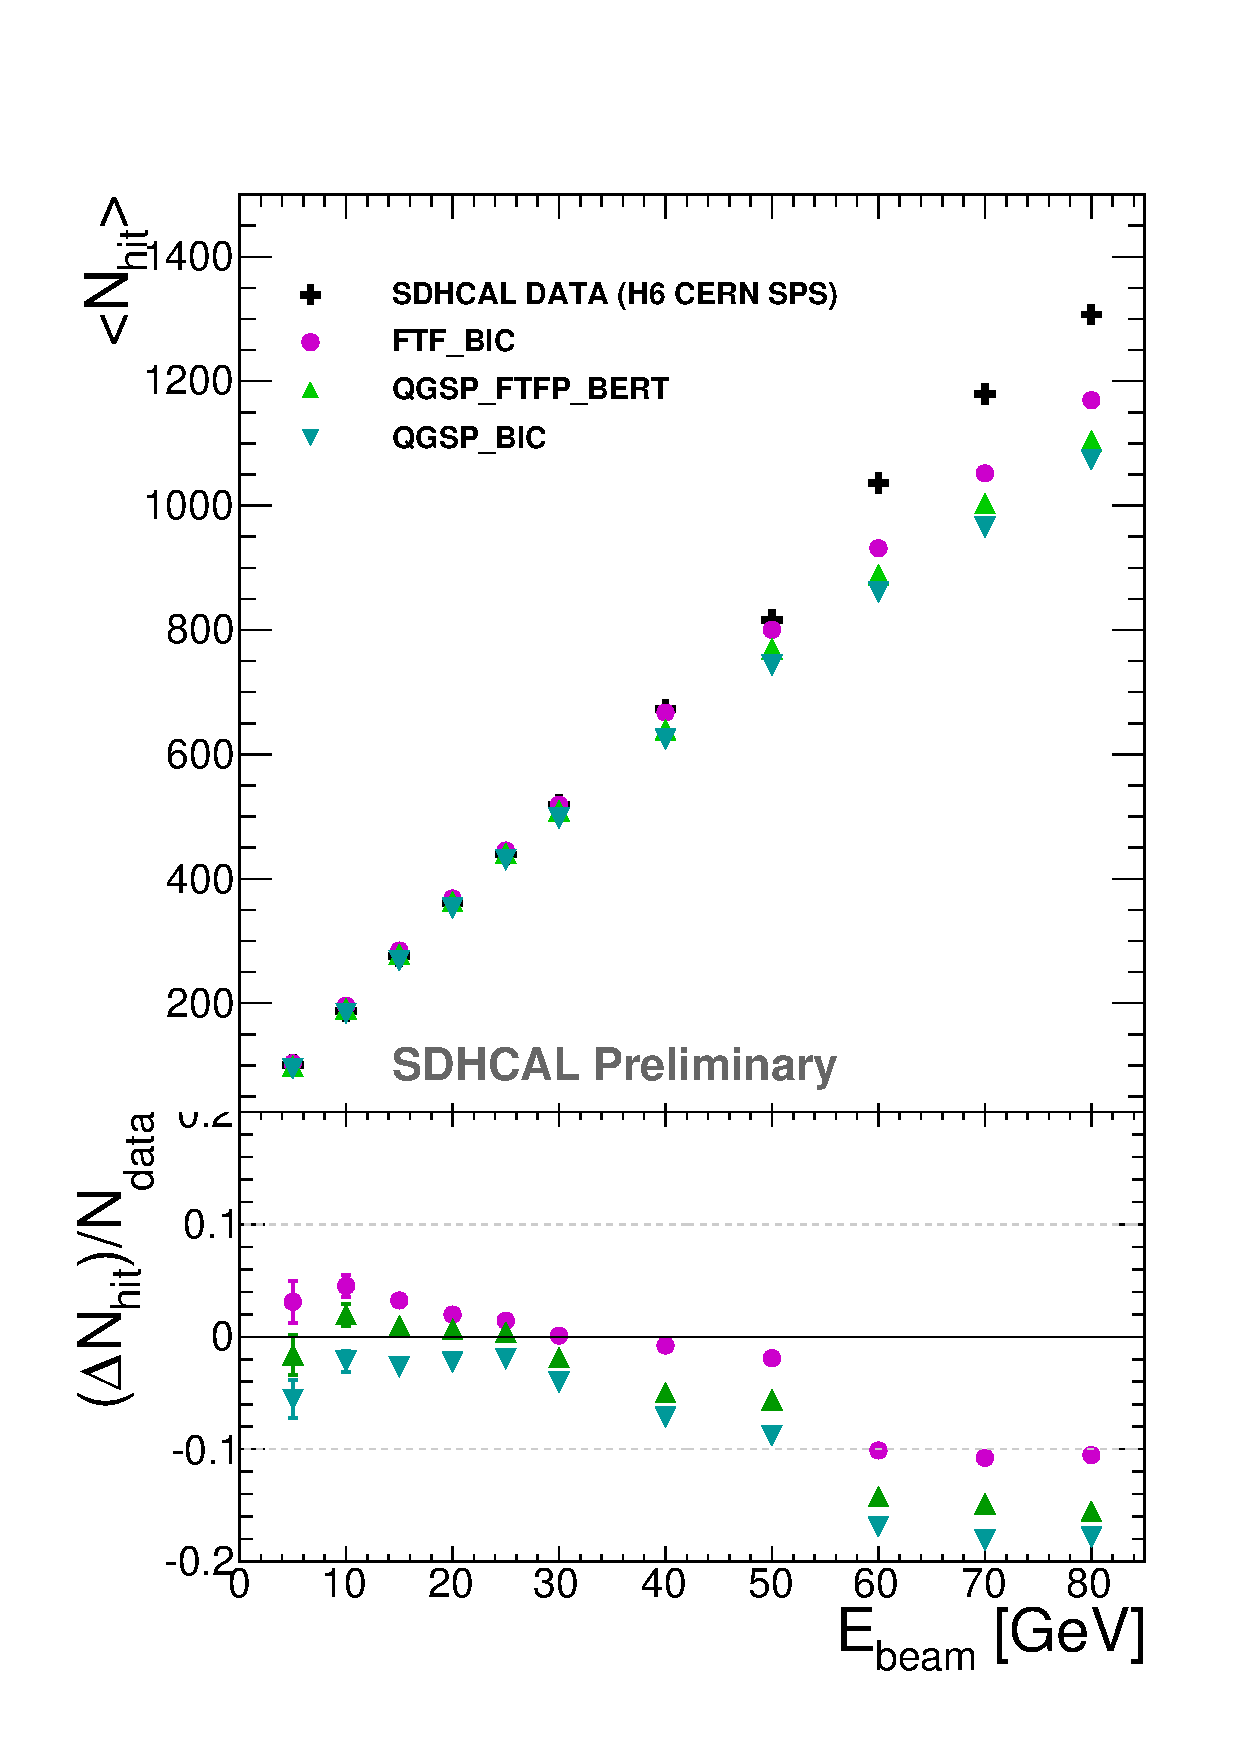
\includegraphics[width=.5\textwidth]{Digitizer/figs/NHITPION_MODEL.pdf}
  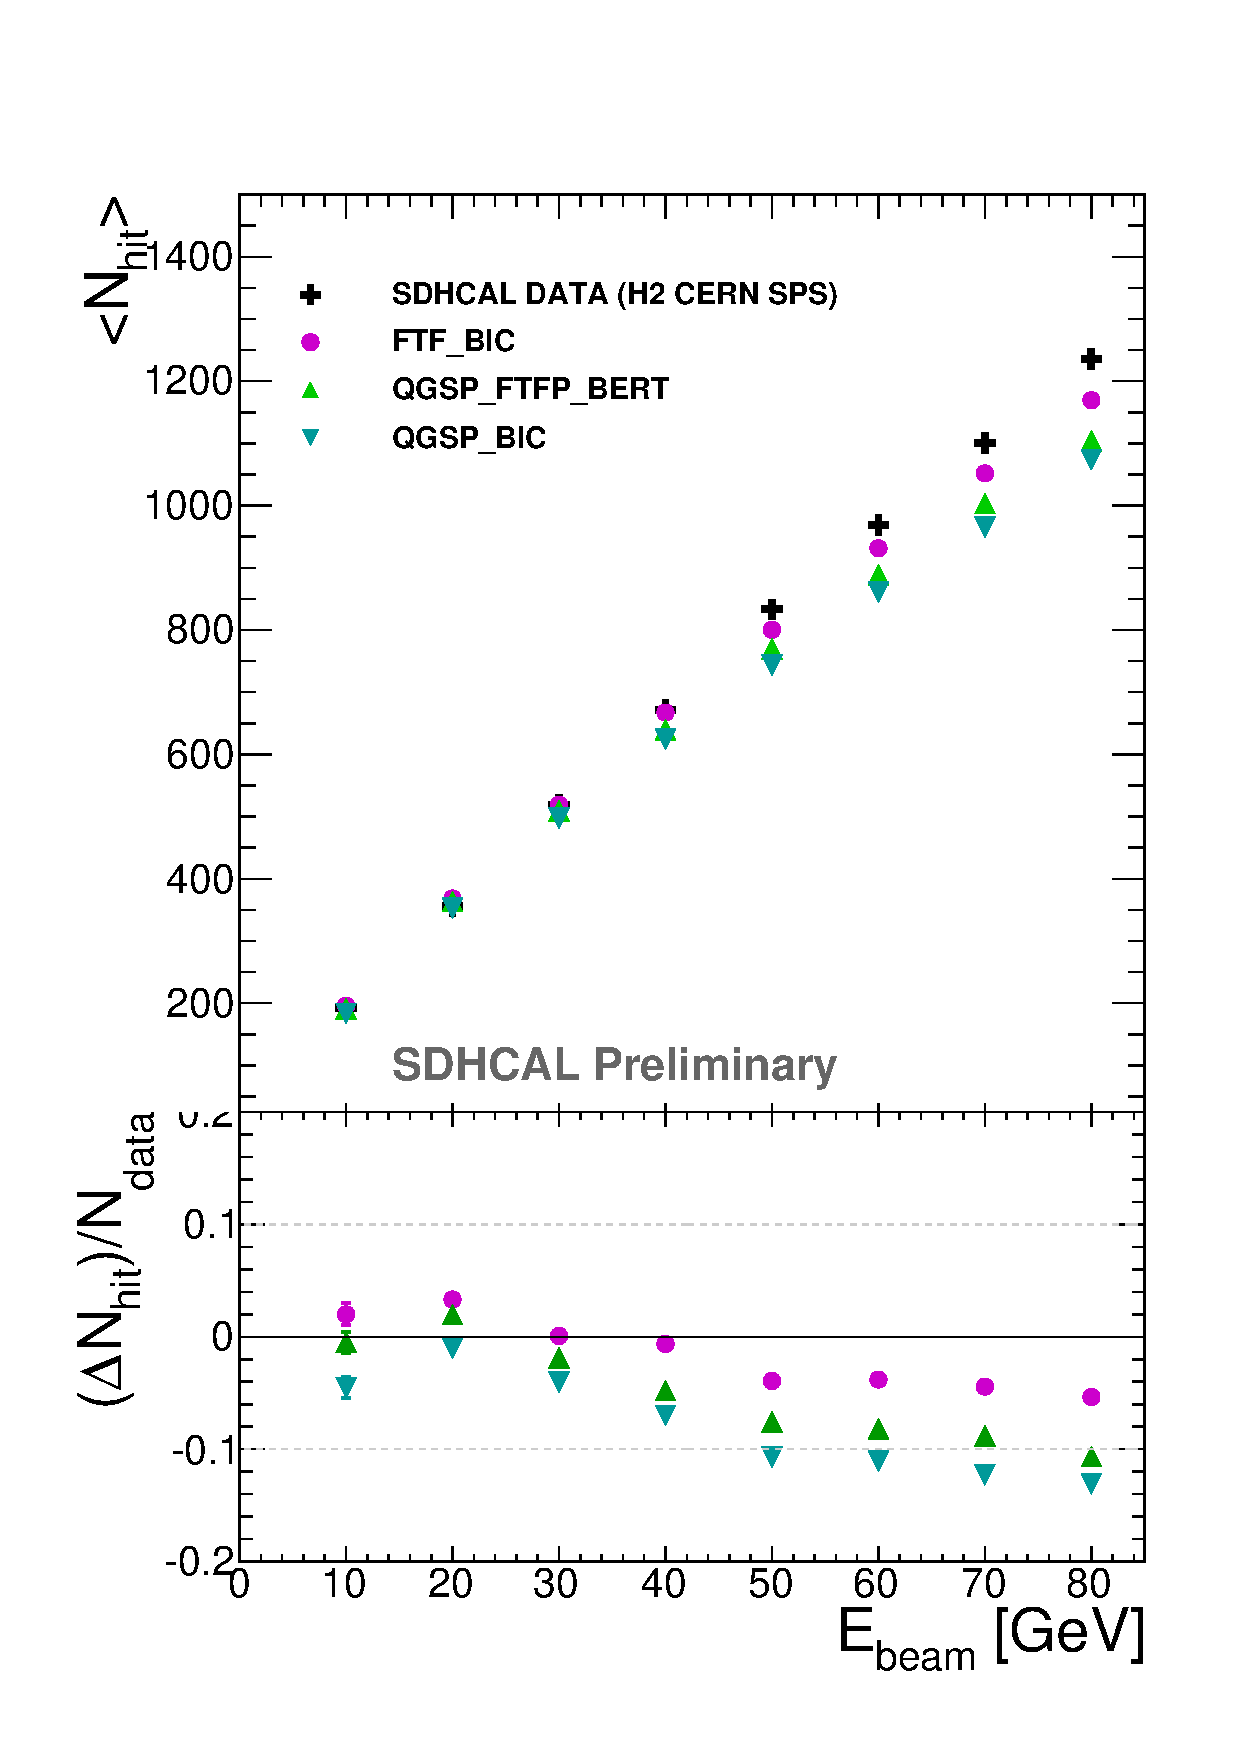
\includegraphics[width=.5\textwidth]{Digitizer/figs/NHITPION_MODEL_NOV.pdf}
  \caption{Nombre moyen de hits pour des gerbes hadroniques en fonction de l'énergie du faisceau pour les données (croix noires) enregistrées sur les lignes H6 (à gauche) et H2 (à droite) et les listes physiques FTF\_BIC (cercles roses), QGSP\_FTFP\_BERT (triangles verts) et QGSP\_BIC (triangle cyans). Les déviations relatives sont aussi présentées.}
  \label{fig.nhit_pi-_ebeam_model}
\end{figure}
D'autres listes physiques préparées par GEANT4 sont aussi testées. La figure~\ref{fig.nhit_pi-_ebeam_model} présente le nombre moyen de hits en fonction de l'énergie pour les listes physiques FTF\_BIC, QGSP\_FTFP\_BERT et QGSP\_BIC et pour les données enregistrées sur les lignes H2 et H6. La liste FTF\_BIC est en meilleur accord avec les données expérimentales, particulièrement à haute énergie. Au delà de 60 $GeV$, le nombre de hits reste sous-estimé. Enfin, notons que la collaboration GEANT4 a corrigé un problème dans le modèle de Fritiof à partir de la version 10.1\footnote{\url{http://geant4.web.cern.ch/geant4/support/Beta4.10.1-1.txt}}. Le fragmentation des cordes hadroniques du modèle de Fritiof produit dorénavant plus de pions neutres et moins de pions chargés. La correction augmente la composante électromagnétique des cascades. Les premiers tests avec cette nouvelle version de GEANT4 n'ont cependant pas montré d'amélioration très significative.

Sur les figures~\ref{fig.nhit_pi-_ebeam} et \ref{fig.nhit_pi-_ebeam_model}, on constate que le nombre de hits augmente brutalement à partir de 60 $GeV$ pour les données enregistrées sur la ligne H6. Cet effet n'est pas présent pour les données de la ligne H2 et est probablement causé par la contamination de la ligne H6 par les protons. 
\begin{figure}[!ht]
  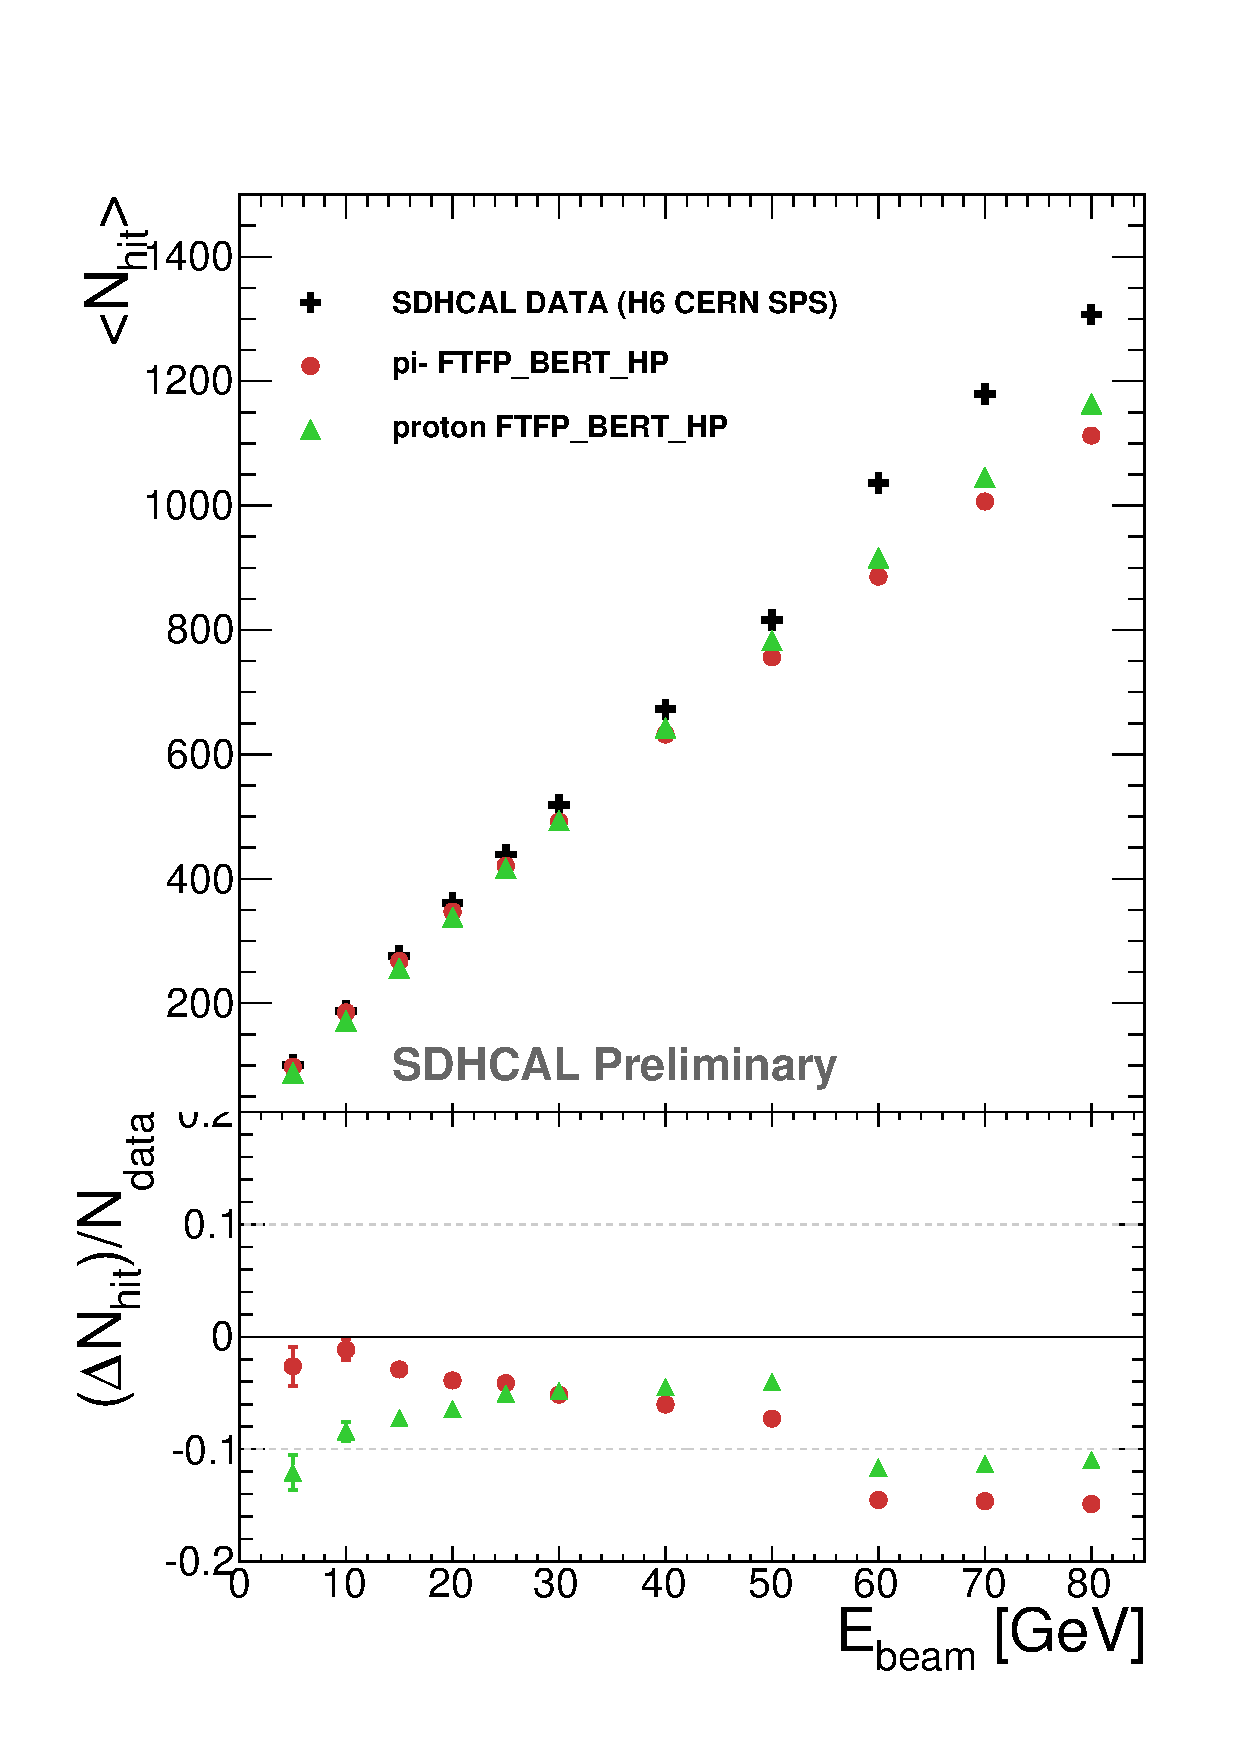
\includegraphics[width=.5\textwidth]{Digitizer/figs/NHITPROTON.pdf}
  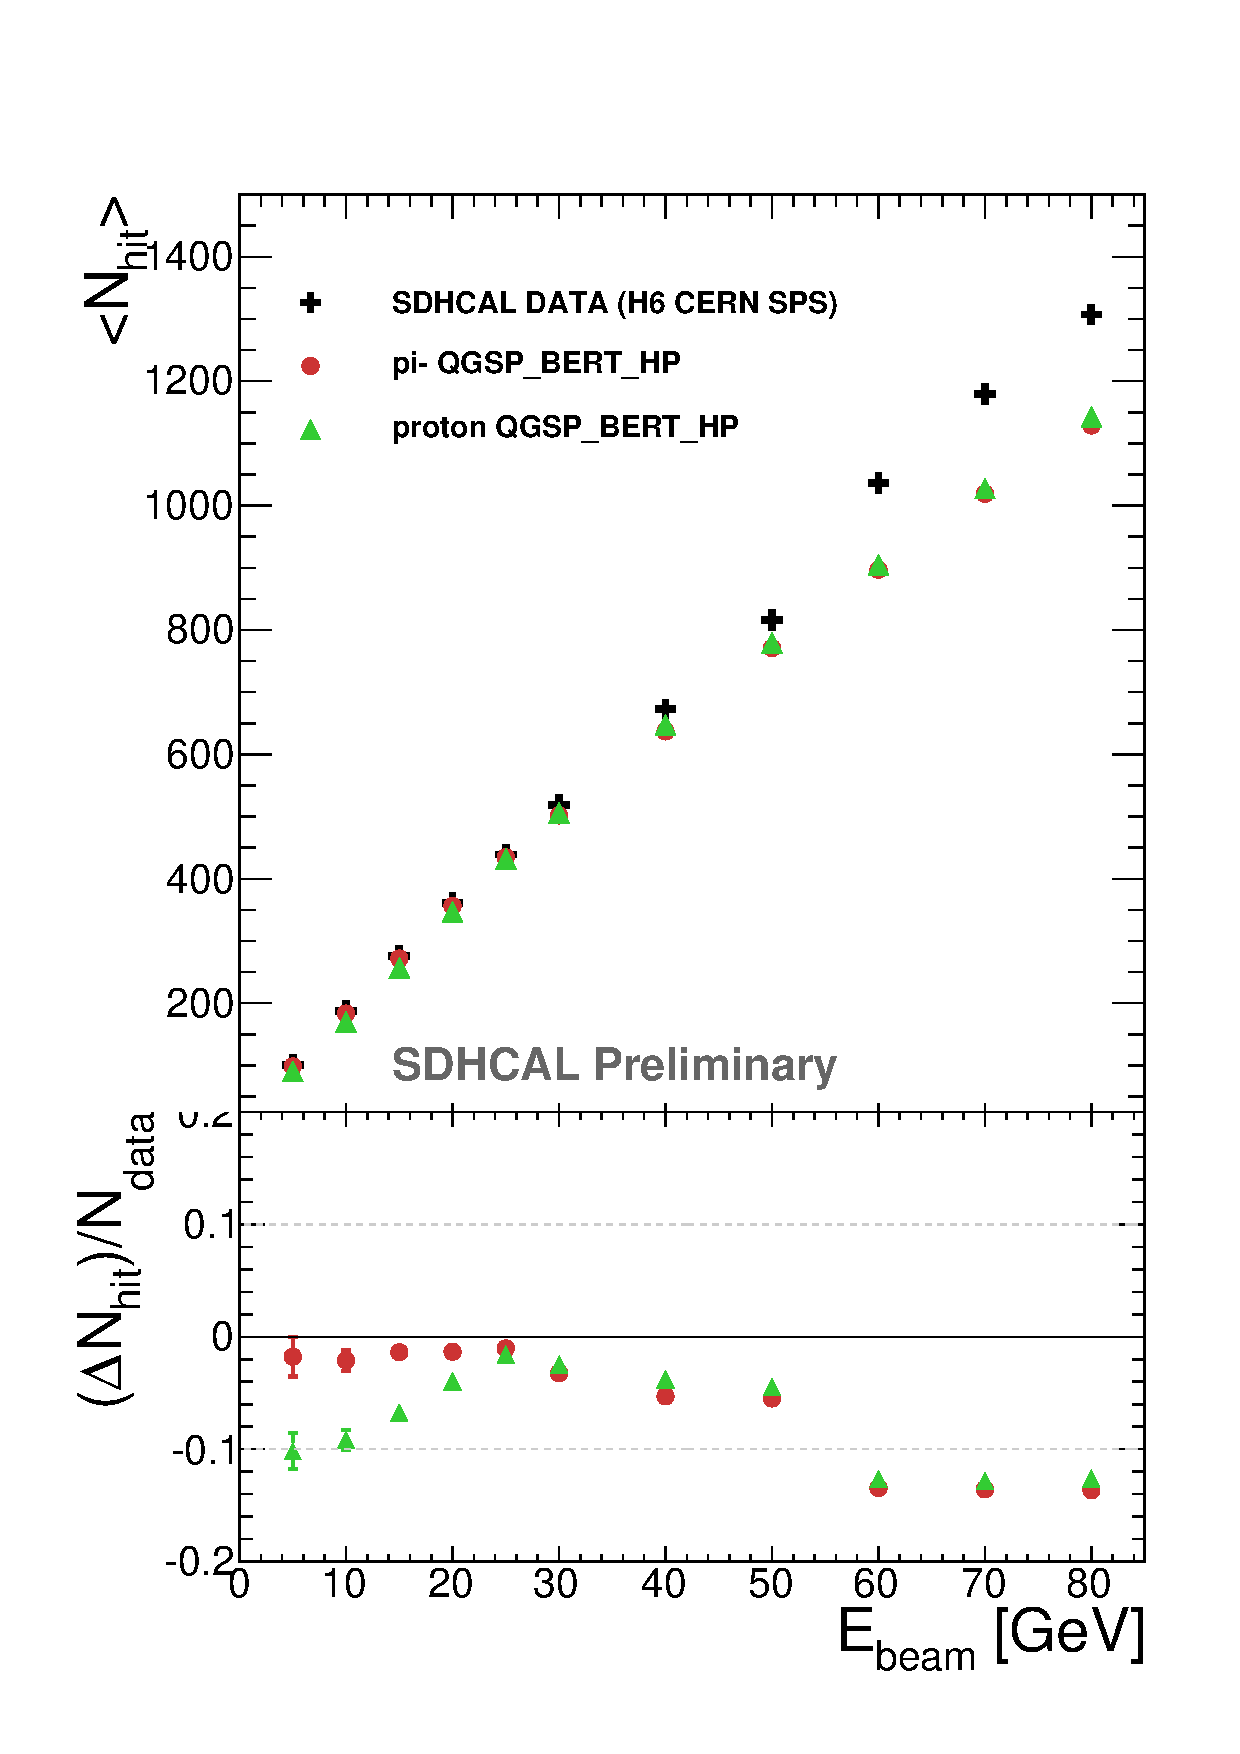
\includegraphics[width=.5\textwidth]{Digitizer/figs/NHITPROTON_QGSP.pdf}
  \caption{Nombre moyen de hits pour les gerbes hadroniques en fonction de l'énergie du faisceau pour les données de la ligne H6 (croix noires), pour les gerbes hadroniques initiées par des pions (cercles rouges) et par des protons (triangles verts) simulées avec les listes physiques FTFP\_BERT\_HP (à gauche) et QGSP\_BERT\_HP (à droite). Les déviations relatives sont aussi présentées.}
  \label{fig.nhit_proton_ebeam}
\end{figure}
La figure~\ref{fig.nhit_proton_ebeam} montre le nombre total moyen de hits pour les données de la ligne H6, pour une simulation de pions et de protons avec les listes physiques FTFP\_BERT\_HP et QGSP\_BERT\_HP. Au dessus de 40 $GeV$, le nombre total de hits est légèrement plus élevé pour les gerbes hadroniques initiées par des protons que par des pions. Plusieurs facteurs permettent d'expliquer ces différences. La fraction électromagnétique des gerbes hadroniques initiées par des protons est généralement plus faible que pour celles initiées par des pions (cf. section~\ref{sec.fem} du chapitre~\ref{chap.shower}). Ainsi la saturation de la réponse du SDHCAL est plus faible avec les cascades initiées par des protons. De plus, la longueur d'interaction est plus faible pour les protons que pour les pions ($\lambda_I^{\pi}/\lambda_I^p=1.25$ dans l'acier). La fraction d'énergie qui s'échappe du détecteur est donc plus faible pour les protons que pour les pions. Cependant, le nombre de hits pour une simulation de protons reste toujours significativement plus faible que dans les données à haute énergie. La déviation relative est supérieure à 10$\%$ au dessus de 60 $GeV$. 

\begin{figure}[!ht]
  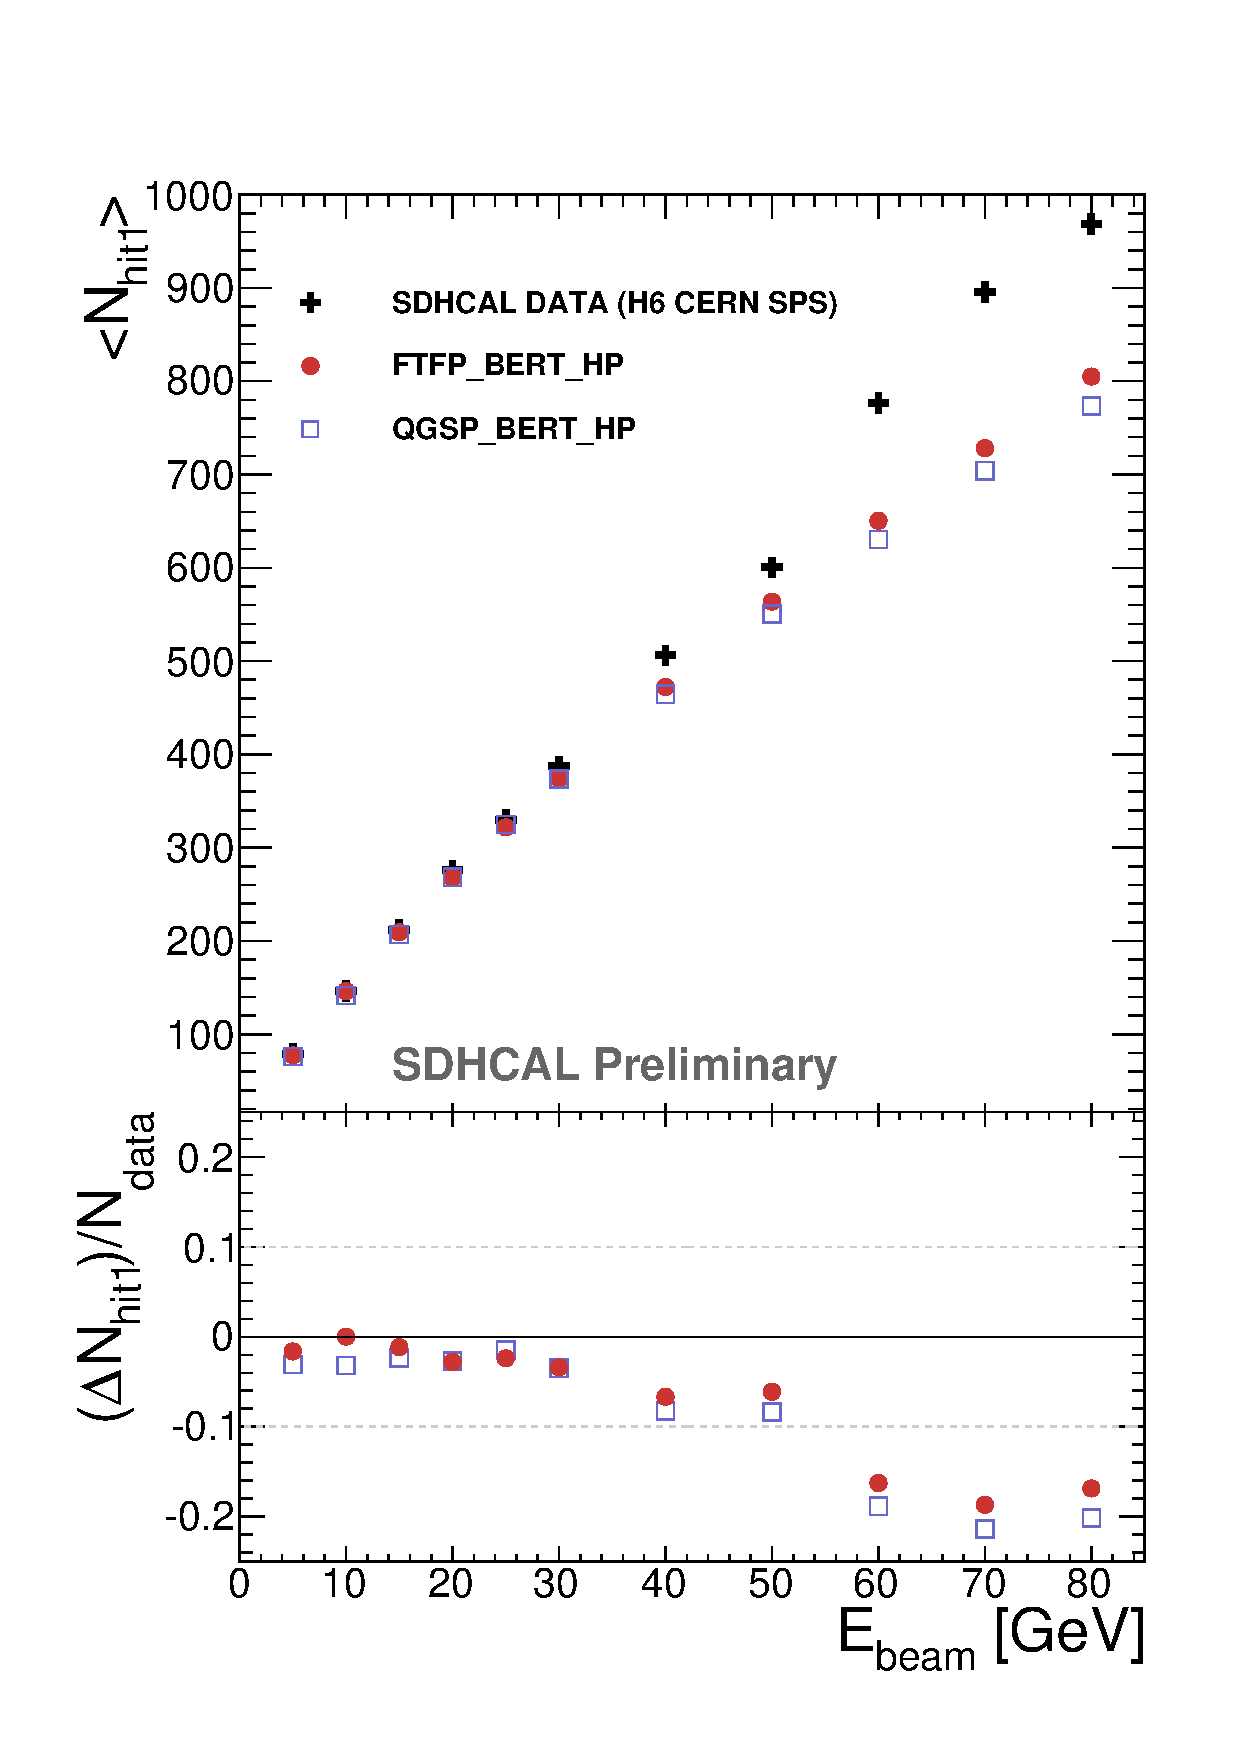
\includegraphics[width=.32\textwidth]{Digitizer/figs/NHIT1PIONHP.pdf}
  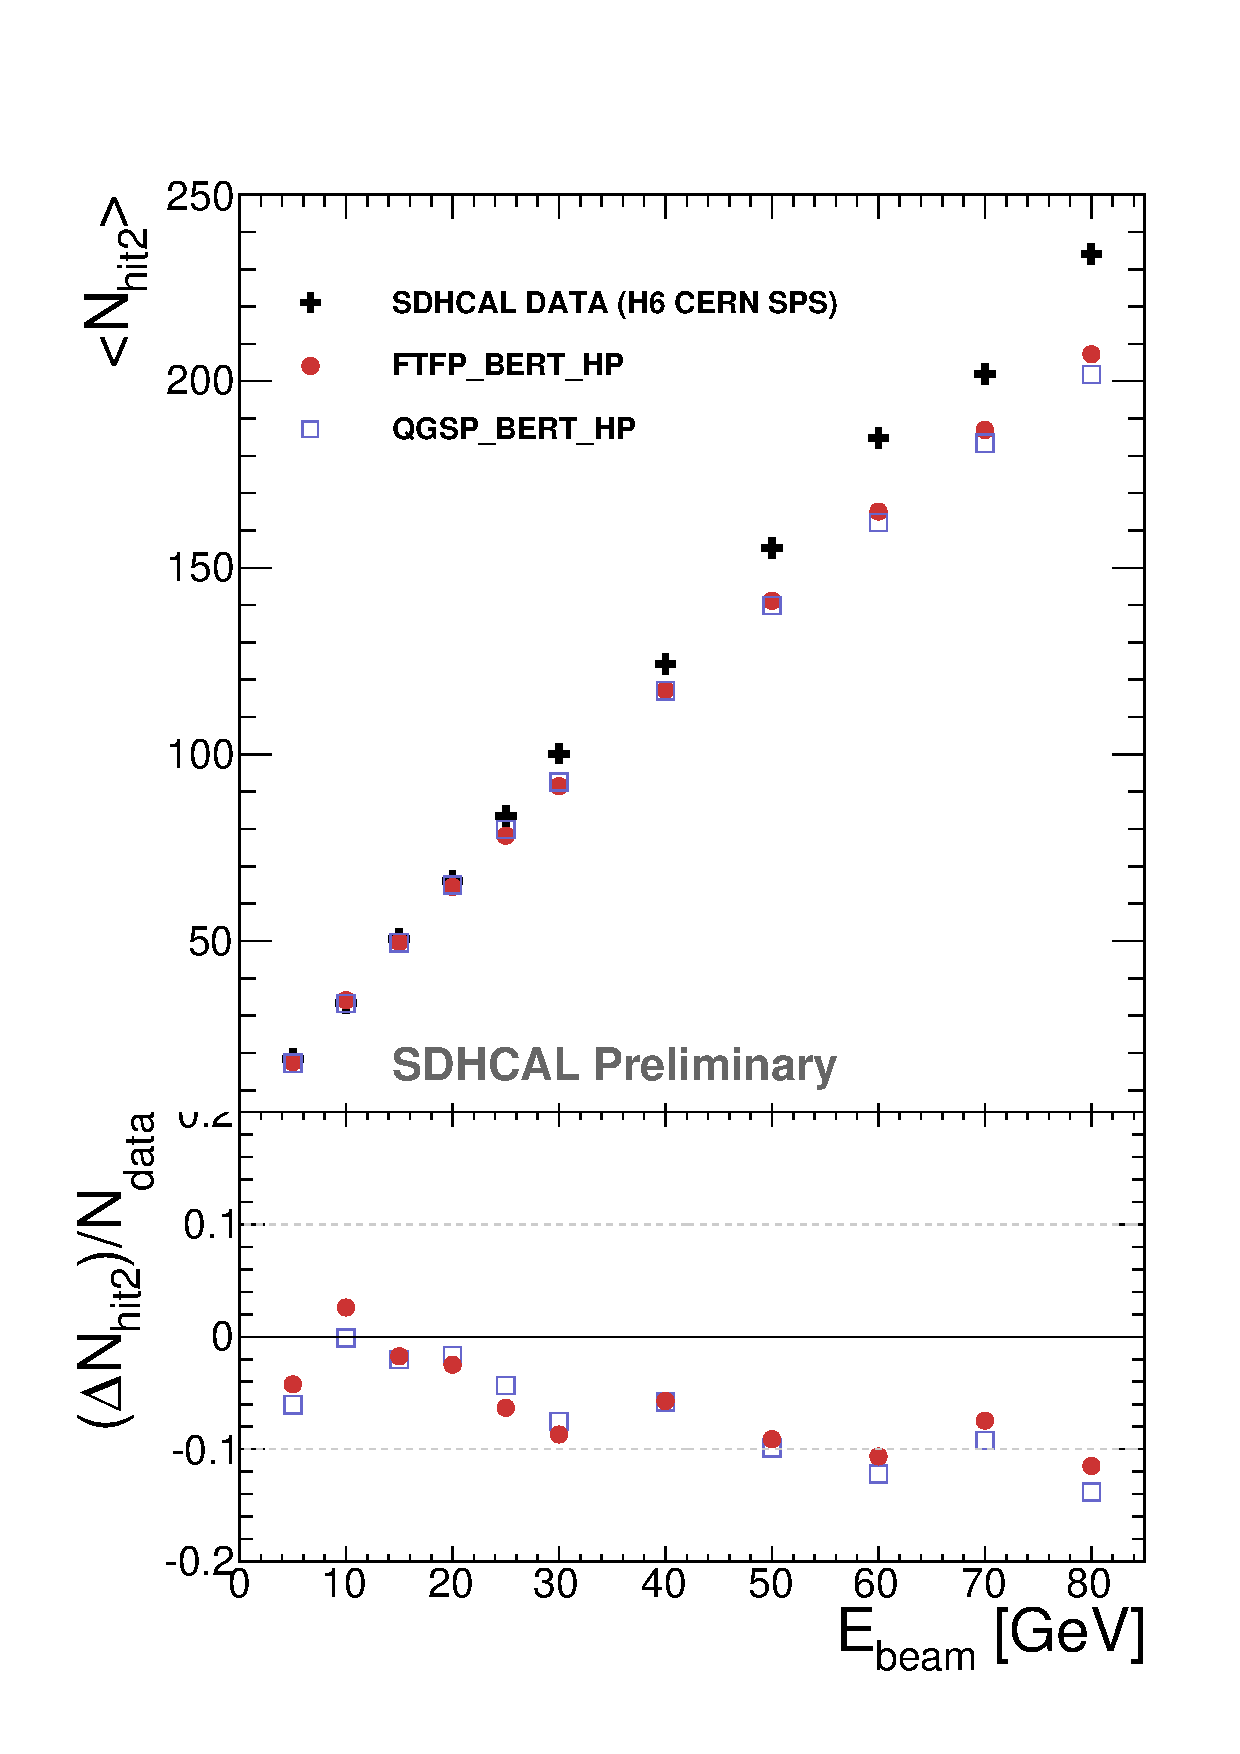
\includegraphics[width=.32\textwidth]{Digitizer/figs/NHIT2PIONHP.pdf}
  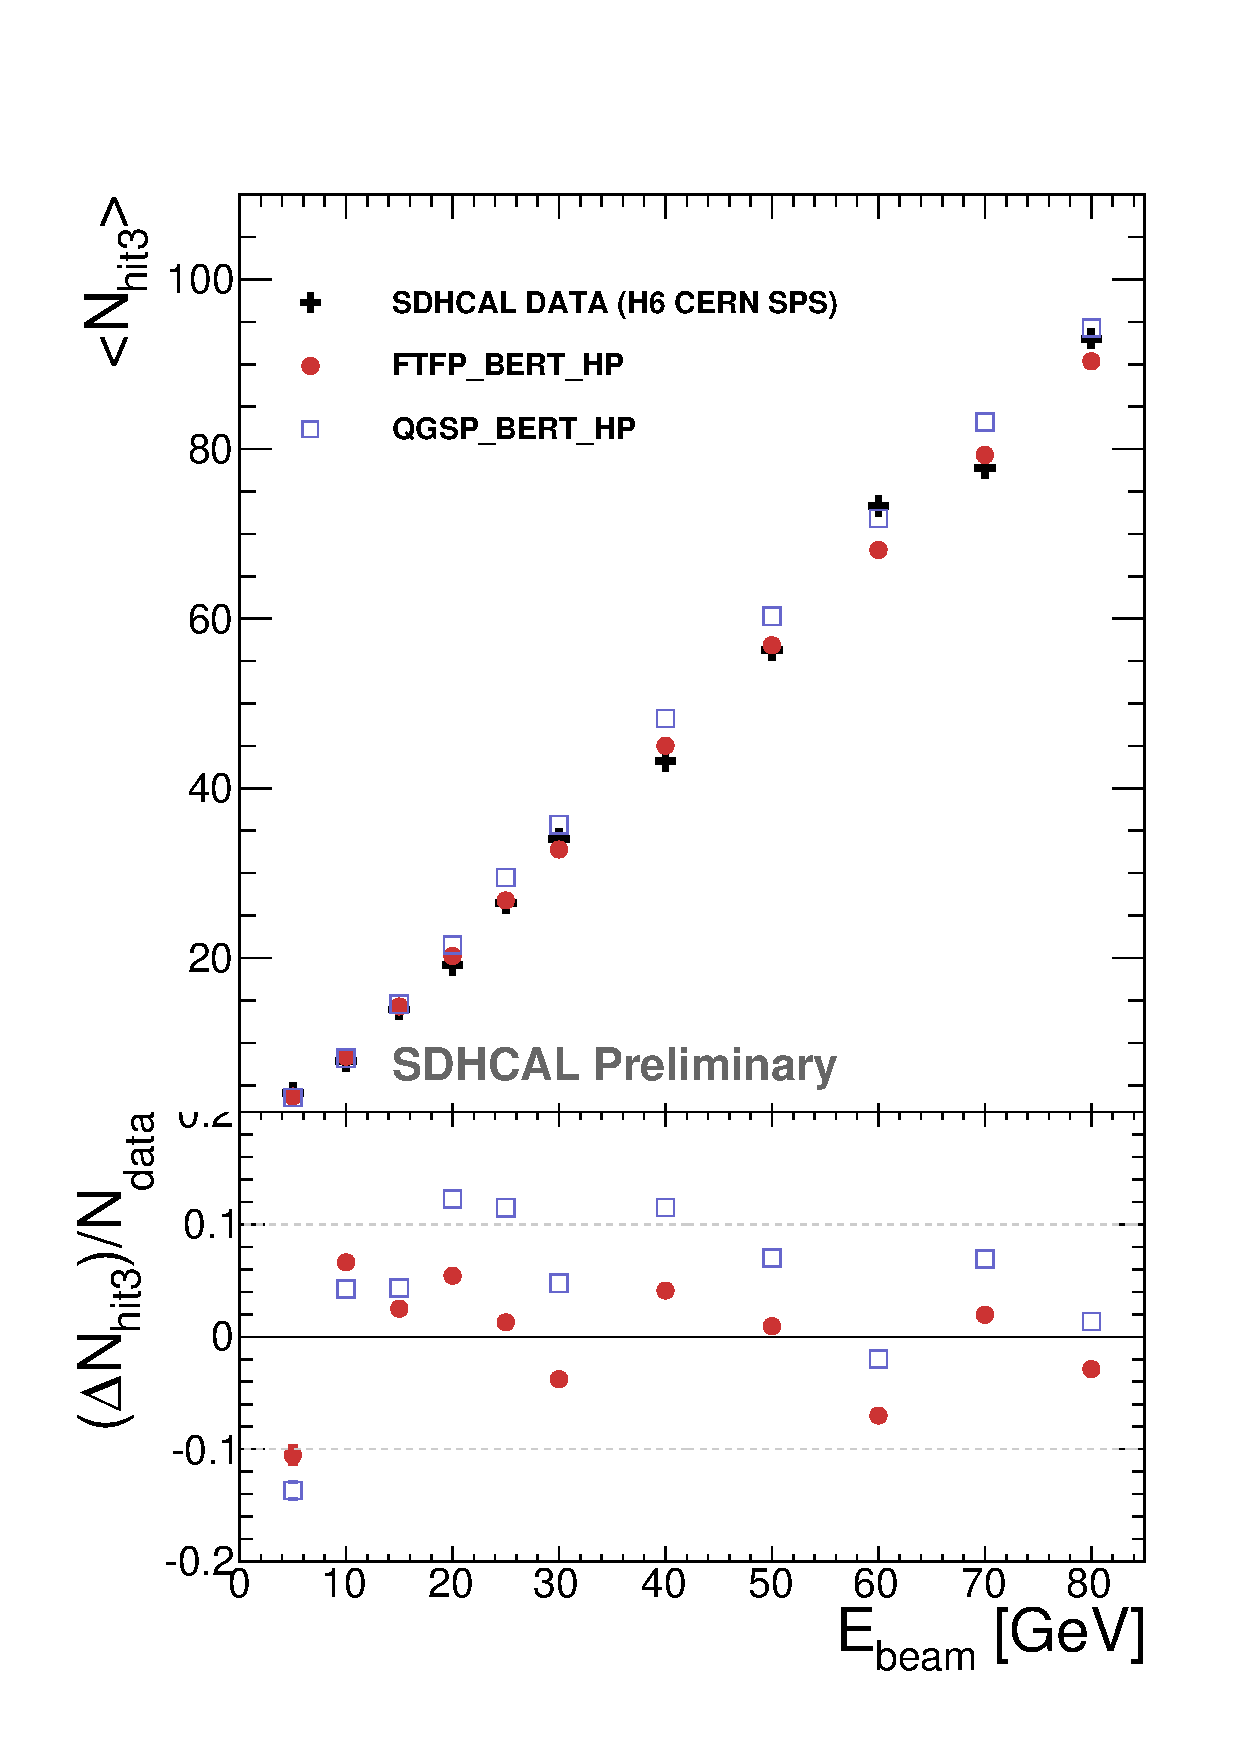
\includegraphics[width=.32\textwidth]{Digitizer/figs/NHIT3PIONHP.pdf}
  \caption{Nombre moyen de hits pour chaque seuil en fonction de l'énergie du faisceau. Les données sont représentées par des croix noires et la simulation par des cercles rouges (FTFP\_BERT\_HP) et des carrés bleus (QGSP\_BERT\_HP).\label{fig.pi-nhit_thr}}
\end{figure}
Le nombre de hits pour chaque seuil est aussi étudié. La figure~\ref{fig.pi-nhit_thr} montre le nombre moyen de hits pour chaque seuil, pour les données et la simulation. Le nombre de hits pour les seuils 1 et 2 respectent la même tendance que pour le nombre total de hits: l'accord entre les données et la simulation est raisonnable à basse énergie et se dégrade sensiblement au dessus de 40 $GeV$. Le nombre de hits pour le troisième seuil est la variable la plus sensible aux fluctuations de température et de pression. Ces fluctuations sont équivalentes à des  variations de tension dans le gaz\footnote{Lors des tests en faisceau de 2015, la procédure de correction de la tension en fonction de la température et de la pression a été réalisée afin de limiter cet effet.}. Ceci permet d'expliquer le comportement de cette observable pour les données. Il est ainsi délicat de tirer des conclusions avec cette variable. Cependant, on peut constater que la liste physique QGSP\_BERT\_HP produit légèrement plus de hits seuil 3 que la liste FTFP\_BERT\_HP. Ceci est dû à la gamme de validité du modèle de Bertini qui est plus étendue pour la liste QGSP\_BERT\_HP que pour FTFP\_BERT\_HP. Ce modèle a tendance à créer beaucoup de particules secondaires et donc d'augmenter les hits seuil 3.

%%%%%%%%%%%%%%%%%%%%%%%%%%%%%%%%%%%%%%%%%%%%%%%

\section{Conclusion}
Les différentes étapes de la simulation du prototype et de la modélisation de la réponse des GRPC ont été détaillées. Le paramétrage de l'algorithme SimDigital a été réalisée grâce aux études menées sur la réponse des muons dans le détecteur. Les gerbes électromagnétiques ont aussi été utilisées pour ce paramétrage. Les comparaisons entre données expérimentales et la simulation de gerbes électromagnétiques dans le SDHCAL montrent un accord très satisfaisant. Cela permet de valider la procédure de simulation du prototype et l'algorithme de modélisation de sa réponse aux particules chargées. Cependant, des désaccords sont observés entre les données et la simulation des gerbes hadroniques. Plusieurs modèles de simulation préparés par la collaboration GEANT4 ont été testés. La liste FTF\_BIC est la liste présentant le meilleur accord sur le nombre total de hits avec les données expérimentales. 

Des études similaires ont été menées par les collaborations ATLAS~\cite{Abat} et CALICE~\cite{geant4-ahcal} avec des calorimètres utilisant une autre technologie. Ces études ont montré que les listes physiques FTFP\_BERT\_HP et QGSP\_BERT\_HP simulent correctement la réponse de ces détecteurs au passage de gerbes hadroniques. Cependant ces deux calorimètres utilisent des scintillateurs comme milieu actif et ont une lecture analogique. Le signal de ces scintillateurs est proportionnel à l'énergie déposée par les particules chargées. De plus, la segmentation transverse de ces deux calorimètres est moins fine que pour le SDHCAL. Ceci pourrait expliquer pourquoi la réponse simulée dans le SDHCAL est plus faible que dans les données, alors que celle-ci est en bon accord pour les détecteurs ATLAS-TileCal et CALICE-AHCAL.
